\item 用列举法表示下列集合:\\
(1) 十二生肖组成的集合;\\
(2) 中国国旗上所有颜色组成的集合.
\item 用描述法表示下列集合:\\
(1) 平面直角坐标系中第一象限的角平分线上的所有点组成的集合;\\
(2) $3$的所有倍数组成的集合.
\item (1) 若$\alpha$: $x^2-5x+6=0$, $\beta$: $x=2$, 则$\alpha$是$\beta$的\blank{50}条件;
(2) 若$\alpha$: 四边形$ABCD$是正方形, $\beta$: 四边形$ABCD$的两条对角线互相垂直平分, 则$\alpha$是$\beta$的\blank{50}条件.
\item 已知方程$x^2+px+4=0$的所有解组成的集合为$A$, 方程$x^2+x+q=0$的所有解组成的集合为$B$, 且$A\cap B=\{4\}$. 求集合$A\cup B$的所有子集.
\item 已知集合$A=(-2, 1)$, $B=(-\infty, -2)\cup [1, +\infty)$. 求: $A\cup B$, $A\cap B$.
\item 已知全集$U=(-\infty, 1)\cup [2, +\infty)$, 集合$A=(-1, 1)\cup [3, +\infty)$. 求$\overline{A}$.
\item 已知集合$A=\{x|x^2+px+q=0\}$, $B=\{x|x^2-x+r=0\}$, 且$A\cap B=\{-1\}$, $A\cup B=\{-1, 2\}$. 求实数$p$、$q$、$r$的值.
\item 设$a$是实数. 若$x=1$是$x>a$的一个充分条件, 则$a$的取值范围为\blank{50}.
\item 已知陈述句$\alpha$是$\beta$的充分非必要条件. 若集合$M=\{x|x\text{满足}\alpha\}$, $N=\{x|x\text{满足}\beta\}$, 则$M$与$N$的关系为\bracket{20}.
\fourch{$M\subset N$}{$M\supset N$}{$M=N$}{$M\cap N=\varnothing$}
\item 证明: 若梯形的对角线不相等, 则该梯形不是等腰梯形.
\item 若集合$M=\{a|a=x+\sqrt2y, x,y\in \mathbf{Q}\}$, 则下列结论正确的是\bracket{20}.
\fourch{$M\subseteq \mathbf{Q}$}{$M=\mathbf{Q}$}{$M\supset \mathbf{Q}$}{$M\subset \mathbf{Q}$}
\item 若$\alpha$是$\beta$的必要非充分条件, $\beta$是$\gamma$的充要条件, $\gamma$是$\delta$的必要非充分条件, 则$\delta$是$\alpha$的\blank{50}条件, $\gamma$是$\alpha$的\blank{50}条件.
\item 已知全集$U=\{x|x\text{为不大于}20\text{的素数}\}$. 若$A\cap \overline{B}=\{3, 5\}$, $\overline{A}\cap B=\{7, 19\}$, $\overline{A\cup B}=\{2, 17\}$, 则A=\blank{50} , B=\blank{50}.
\item 已知集合$P=\{x|-2\le x\le 5\}$, $Q=\{x|x\ge k+1\text{且}x\le 2k-1\}$, 且$Q\subseteq P$. 求实数$k$的取值范围.
\item 已知全集$U=\mathbf{R}$, 集合$A=\{x|x\le a-1\}$, $B=\{x|x>a+2\}$, $C=\{x|x<0\text{或}x\ge 4\}$, 且$\overline{A\cup B}\subseteq C$. 求实数$a$的取值范围.
\item 已知集合$A=\{x|(a-1)x^2+3x-2=0\}$. 是否存在这样的实数$a$, 使得集合$A$有且仅有两个子集? 若存在, 求出实数$a$的值及对应的两个子集; 若不存在, 说明理由.
\item 证明: $\sqrt[3]{2}$是无理数.
\item 设$a,b$是正整数. 求证: 若$ab-1$是$3$的倍数, 则$a$与$b$被$3$除的余数相同.
\item 已知非空数集$S$满足: 对任意给定的$x,y\in S$($x,y$可以相同), 有$x+y\in S$且$x-y\in S$.\\
(1) 哪个数一定是$S$中的元素? 说明理由;\\
(2) 若$S$是有限集, 求$S$;\\
(3) 若$S$中最小的正数为$5$, 求$S$.
\item 设一元二次方程$2x^2-6x-3=0$的两个实根为$x_1,x_2$, 求下列各式的值:\\
(1) $(x_1+1)(x_2+1)$;\\
(2) $(x_1^2-1)(x_2^2-1)$.
\item 设$a>b>0$, 比较$\dfrac{b+2a}{a+2b}$与$\dfrac ab$的值的大小.
\item 已知$x>y$, 求证: $x^3-y^3>x^2y-xy^2$.
\item 若关于$x$的不等式$(a+1)x-a<0$的解集为$(2,+\infty)$, 求实数$a$的值, 并求不等式$(a-1)x+3-a>0$的解集.
\item 解下列一元二次不等式:\\
(1) $-x^2+11<-2x-4$;\\
(2) $3x^2<13x+10$;\\
(3) $6x+2\ge 5x^2$;\\
(4) $x^2\le 8(1-x)$;\\
(5) $-x^2\ge 9(9-2x)$;\\
(6) $3(x-3)\le x^2$.
\item 试写出一个二次项系数为$1$的一元二次不等式, 使它的解集分别为:\\
(1) $(-\infty, \sqrt 2)\cup  (\sqrt 2, +\infty)$;\\
(2) $[2-\sqrt 3, 2+\sqrt 3]$.
\item 求不等式$5\le x^2-2x+2<26$的所有正整数解.
\item 解下列分式不等式:\\
(1) $\dfrac{2x+1}{x+7}>-3$;\\
(2) $\dfrac{3x}{x^2+2}\ge 1$.
\item 设关于$x$的不等式$a_1x^2+b_1x+c_1>0$与$a_2x^2+b_2x+c_2>0$的解集分别为$A$、$B$,
试用集合运算表示下列不等式组的解集:\\
(1) $\begin{cases} a_1x^2+b_1x+c_1>0, \\ a_2x^2+b_2x+c_2>0;\end{cases}$\\
(2) $\begin{cases} a_1x^2+b_1x+c_1\le 0, \\ a_2x^2+b_2x+c_2>0;\end{cases}$\\
(3) $\begin{cases} a_1x^2+b_1x+c_1\le 0, \\ a_2x^2+b_2x+c_2\le 0.\end{cases}$
\item 解下列含绝对值的不等式:\\
(1) $|2x-1|\le x$;\\
(2) $|2x+1|+|x-2|<8$.
\item 已知$a$、$b$是正数, 求证: $\sqrt{(1+a)(1+b)}\ge 1+\sqrt{ab}$.
\item 如图, 在直角三角形$ABC$中, $AD$垂直于斜边$BC$, 且垂足为$D$. 设$BD$及$CD$的长度分别为$a$与$b$.\\
(1) 求斜边上的高$AD$与中线$AE$的长;\\
(2) 用不等式表示斜边上的高$AD$与中线$AE$长度的大小关系.
\begin{center}
    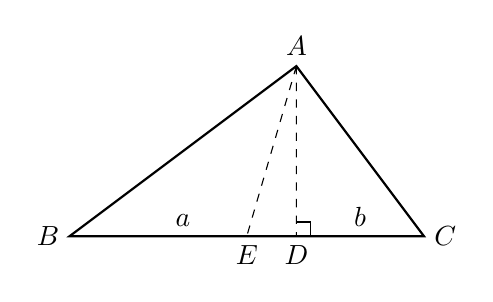
\begin{tikzpicture}[scale = 1.8]
        \draw [thick] (0,0) node [left] {$B$} -- (2.5,0) node [right] {$C$} -- (1.6,1.2) node [above] {$A$} -- cycle;
        \draw [dashed] (1.6,1.2) -- (1.6,0) node [below] {$D$} (1.6,1.2) -- (1.25,0) node [below] {$E$};
        \draw [thin] (1.7,0) -- (1.7,0.1) -- (1.6,0.1);
        \draw (0.8,0) node [above] {$a$} (2.05,0) node [above] {$b$};
    \end{tikzpicture}
\end{center}
\item 如图, 已知直角梯形$ABCD$的顶点$A(a, 0)$、$B(b, 0)$位于$x$轴上, 顶点$C$、$D$落在函数$y=|x|$的图像上, $M$、$N$分别为线段$AB$、$CD$的中点, $O$为坐标原点, $Q$为线段$OC$与线段$MN$的交点.\\
(1) 求中点$M$的坐标, 以及线段$MQ$、$MN$的长度;\\
(2) 用不等式表示$MQ$、$MN$长度的大小关系.
\begin{center}
    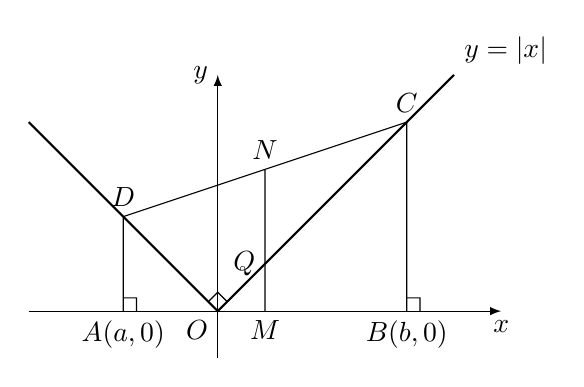
\begin{tikzpicture}[scale = 1.2,>=latex]
        \draw [->] (-2,0) -- (3,0) node [below] {$x$};
        \draw [->] (0,-0.5) -- (0,2.5) node [left] {$y$};
        \draw (0,0) node [below left] {$O$};
        \draw [thick] (-2,2) -- (0,0) -- (2.5,2.5) node [above right] {$y=|x|$};
        \draw [thin] (-0.1,0.1) -- (0,0.2) -- (0.1,0.1) (2.14,0) -- (2.14,0.14) -- (2,0.14) (-0.86,0) -- (-0.86,0.14) -- (-1,0.14);
        \draw (-1,0) node [below] {$A(a,0)$} -- (-1,1) node [above] {$D$} -- (0.5,1.5) node [above] {$N$} -- (2,2) node [above] {$C$} -- (2,0) node [below] {$B(b,0)$} (0.5,1.5) -- (0.5,0.5) node [left] {$Q$} -- (0.5,0) node [below] {$M$}; 
    \end{tikzpicture}
\end{center}
\item 已知一元二次方程$x^2+px+p=0$的两个实根分别为$\alpha$、$\beta$, 且$\alpha^2$+$\beta^2=3$, 求实数$p$的值.
\item 已知一元二次方程$2x^2-4x+m+3=0$有两个同号实根, 求实数$m$的取值范围.
\item 设$a,b\in \mathbf{R}$, 已知关于$x$的不等式$(a+b)x+(b-2a)<0$的解集为$(1, +\infty)$, 求不等式$(a-b)x+3b-a>0$的解集.
\item 解下列不等式:\\
(1) $-2< \dfrac 1{2x+1}\le 3$;\\
(2) $2<|x+1|\le 3$.
\item 已知集合$A=\{x||x-a|<2\}$, $B=\{x|\dfrac{2x-1}{x+2}<1\}$, 且$A\subseteq B$. 求实数$a$的取值范围.
\item 证明: 若$x>-1$, 则$x+\dfrac 1{x+1}\ge 1$, 并指出等号成立的条件.
\item 设$a$、$b$为正数, 且$a+b=2$. 求$\dfrac 1a+\dfrac 1b$的最小值.
\item 已知$a$、$b$、$c$都是正数, 求证: $\dfrac{b+c}{a}+\dfrac{c+a}{b}+\dfrac{a+b}{c}\ge 6$.
\item 设实数$x$、$y$满足$|x+y|=1$, 求$xy$的最大值.
\item 已知$a$、$b$为实数, 求证:$|a|+|b| \le |a+b| +|a-b|$, 并指出等号成立的条件.
\item 已知$a$、$b$是实数,\\
(1) 求证: $a^2+ab+b^2\ge 0$, 并指出等号成立的条件;\\
(2) 求证: 如果$a>b$, 那么$a^3>b^3$.
\item 解下列不等式:\\
(1) $\dfrac{3x-11}{x^2-6x+9}\le 1$;\\
(2) $|3-2x| \ge |x+1|$.
\item 已知集合$A=\{x|x^2-2x-3>0\}$, $B=\{x|x^2+px+q\le 0\}$. 若$A\cup B=\mathbf{R}$, 且$A\cap B=[-2,-1)$, 求实数$p$及$q$的值.
\item 已知实数$0<a<b$, 求证: $a<\dfrac{2ab}{a+b}<\sqrt{ab}<\dfrac{a+b}{2}<\sqrt{\dfrac{a^2+b^2}{2}}<b$.
\item 方程$(x-1)(x-2)(x-3)=0$的三个根$1$、$2$、$3$将数轴划分为四个区间, 即$(-\infty, 1)$, $(1, 2)$, $(2, 3)$, $(3, +\infty)$. 试在这四个区间上分别考察$(x-1)(x-2)(x-3)$的
符号, 从而得出不等式$(x-1)(x-2)(x-3)>0$与$(x-1)(x-2)(x-3)<0$的解集.\\
一般地, 对$x_1$、$x_2$、$x_3\in \mathbf{R}$, 且$x_1\le x_2\le x_3$, 试分别求不等式$(x-x_1)(x-x_2)(x-x_3)>0$与$(x-x_1)(x-x_2)(x-x_3)<0$的解集(提示: $x_1$、$x_2$、$x_3$相互之间可能相等, 需要分情况讨论).
\item 填空题:\\
(1) 若$x^3=5$, 则$x=$\blank{50}; 若$3^x=5$, 则$x=$\blank{50}.\\
(2) 将$\sqrt[4]{a\sqrt[3]{a}} \ (a>0)$化成有理数指数幂的形式为\blank{50}.\\
(3) 若$\log_8x=-\dfrac 23$, 则$x=$\blank{50}.\\
(4) 若$\log_a b\cdot \log_5 a=3$($a>0$且$a\ne 1$), 则$b=$\blank{50}.
\item 选择题:\\
(1) 若$\lg a$与$\lg b$互为相反数, 则有\bracket{20}.
\fourch{$a+b=0$}{$ab=1$}{$\dfrac ab=1$}{以上答案均不对}
(2) 设$a>0$, 下列计算中正确的是\bracket{20}.
\twoch{$a^\frac{2}{3}\cdot a^\frac{3}{2}=a$}{$a^\frac{2}{3}\div a^\frac{3}{2}=a$}{$a^{-4}\cdot a^4=0$}{$(a^\frac{2}{3})^\frac{3}{2}=a$}
\item 已知$10^\alpha=3$, $10^\beta=4$. 求$10^{\alpha+\beta}$及$10^{\alpha-\frac{\beta}2}$的值.
\item 求下列各式的值:\\
(1) $\dfrac{1}{4^x+1}+\dfrac{1}{4^{-x}+1}$;\\
(2) $4^{\sqrt 2+1}\times 2^{3-2\sqrt 2}\times 8^{-\frac 23}$.
\item 已知$\lg a<1$, 化简$\sqrt{\lg^2 a-\lg \dfrac{a^2}{10}}$.
\item 已知$m=\log_2 10$, 求$2^m-m\lg 2-4$的值.
\item 填空题:\\
(1) 若$4^x=2^{-\frac{1}{2}}$, $4^y=\sqrt[3]{32}$, 则$2x-3y=$\blank{50}.\\
(2) 若$\log_3(\log_4 x)=1$, 则$x=$\blank{50}.\\
(3) 若$3^a=7^b=63$, 则$\dfrac 2a+\dfrac 1b$的值为\blank{50}.\\
\item 已知$\log_{18}9=a$, $18^b=5$, 则$\log_{36}45$等于\bracket{20}.
\fourch{$\dfrac{a+b}{2+a}$}{$\dfrac{a+b}{2-a}$}{$\dfrac{a+b}{2a}$}{$\dfrac{a+b}{a^2}$}
\item 设$\log_{0.2}a>0$, $\log_{0.2}b>0$, 且$\log_{0.2}a\cdot \log_{0.2}b=1$, 求$\log_{0.2}(ab)$的最小值.
\item 化简$\dfrac{(1+2^x)(1+2^{2x})(1+2^{4x})(1+2^{8x})(1+2^{16x})}{1-2^{32x}}$(其中$x\ne 0$).
\item 已知$a>1$, $b>0$. 求证: 对任意给定的实数$k$, $a^{2b+k}-a^{b+k}>a^{b+k}-a^k$.
\item 甲、乙两人同时解关于$x$的方程: $\log_2x+b+c\log_x2=0$. 甲写错了常数$b$, 得两根
$\dfrac 14$及$\dfrac 18$; 乙写错了常数$c$, 得两根$\dfrac 12$及$64$. 求这个方程的真正根.
\item 已知$a$、$b$及$c$是不为$1$的正数, 且$\lg a+\lg b+\lg c=0$. 求证: $a^{\frac{1}{\lg b}+\frac{1}{\lg c}}\cdot b^{\frac{1}{\lg c}+\frac{1}{\lg a}}\cdot c^{\frac{1}{\lg a}+\frac{1}{\lg b}}=\dfrac{1}{1000}$.
\item 填空题:\\
(1) 若点$(2, \sqrt 2)$在幂函数$y=x^a$的图像上, 则该幂函数的表达式为\blank{50}; 若点$(2, \sqrt 2)$在指数函数$y=a^x$($a>0$且$a\ne 1$)的图像上, 则该指数函数的表达式为\blank{50}; 若点$(\sqrt 2, 2)$在对数函数$y=\log_a x$($a>0$且$a\ne 1$)的图像上, 则该对数
函数的表达式为\blank{50}.\\
(2) 若幂函数$y=x^k$在区间$(0, +\infty)$上是严格减函数, 则实数$k$的取值范围为\blank{50}.\\
(3) 已知常数$a>0$且$a\ne 1$, 假设无论$a$为何值, 函数$y=a^{x-2}+1$的图像恒经过一
个定点. 则这个点的坐标为\blank{50}.
\item 选择题:\\
(1) 若指数函数$y=a^x$($a>0$且$a\ne 1$)在$\mathbf{R}$上是严格减函数, 则下列不等式中, 一定能成立的是\bracket{20}.
\fourch{$a>1$}{$a<0$}{$a(a-1)<0$}{$a(a-1)>0$}
(2) 在同一平面直角坐标系中, 一次函数$y=x+a$与对数函数$y=\log_ax$($a>0$且$a\ne 1$)的图像关系可能是\bracket{20}.
\fourch{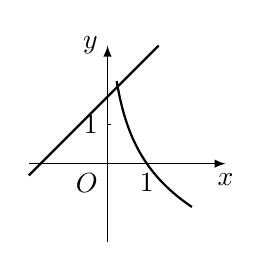
\begin{tikzpicture}[scale = 0.5,>=latex]
    \draw [->] (-2,0) -- (3,0) node [below] {$x$};
    \draw [->] (0,-2) -- (0,3) node [left] {$y$};
    \draw (0,0) node [below left] {$O$};
    \draw (0.1,1) -- (0,1) node [left] {$1$};
    \draw (1,0) node [below] {$1$};
    \draw [thick] (-2,-0.3) -- (1.3,3);
    \draw [thick,domain =-1.1:2.1,samples = 200] plot ({0.5^\x},\x);
\end{tikzpicture}
}{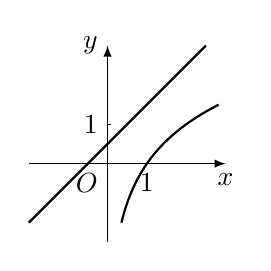
\begin{tikzpicture}[scale = 0.5,>=latex]
    \draw [->] (-2,0) -- (3,0) node [below] {$x$};
    \draw [->] (0,-2) -- (0,3) node [left] {$y$};
    \draw (0,0) node [below left] {$O$};
    \draw (0.1,1) -- (0,1) node [left] {$1$};
    \draw (1,0) node [below] {$1$};
    \draw [thick] (-2,-1.5) -- (2.5,3);
    \draw [thick,domain =1.5:-1.5,samples = 200] plot ({0.5^\x},-\x);
\end{tikzpicture}
}{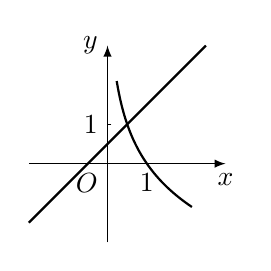
\begin{tikzpicture}[scale = 0.5,>=latex]
    \draw [->] (-2,0) -- (3,0) node [below] {$x$};
    \draw [->] (0,-2) -- (0,3) node [left] {$y$};
    \draw (0,0) node [below left] {$O$};
    \draw (0.1,1) -- (0,1) node [left] {$1$};
    \draw (1,0) node [below] {$1$};
    \draw [thick] (-2,-1.5) -- (2.5,3);
    \draw [thick,domain =-1.1:2.1,samples = 200] plot ({0.5^\x},\x);
\end{tikzpicture}
}{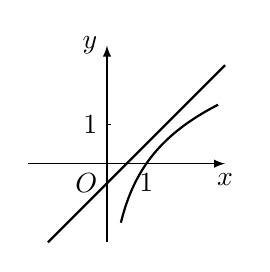
\begin{tikzpicture}[scale = 0.5,>=latex]
    \draw [->] (-2,0) -- (3,0) node [below] {$x$};
    \draw [->] (0,-2) -- (0,3) node [left] {$y$};
    \draw (0,0) node [below left] {$O$};
    \draw (0.1,1) -- (0,1) node [left] {$1$};
    \draw (1,0) node [below] {$1$};
    \draw [thick] (-1.5,-2) -- (3,2.5);
    \draw [thick,domain =1.5:-1.5,samples = 200] plot ({0.5^\x},-\x);
\end{tikzpicture}
}
\item 求下列函数的的定义域:\\
(1) $y=(x-1)^{\frac 52}$;\\
(2) $y=3^{\sqrt{x-1}}$;\\
(3) $y=\lg \dfrac{1+x}{1-x}$.
\item 比较下列各题中两个数的大小:\\
(1) $0.1^{0.7}$与$0.2^{0.7}$;\\
(2) $0.7^{0.1}$与$0.7^{0.2}$;\\
(3) $\log_{0.7}0.1$与$\log_{0.7}0.2$.
\item 设点$(\sqrt 2, 2)$在幂函数$y_1=x^a$的图像上, 点$(-2,\dfrac 14)$在幂函数$y_2=x^b$的图像上. 当$x$取何值时, $y_1=y_2$?
\item 设$a=(\dfrac 23)^x$, $b=x^{\frac 32}$及$c=\log_\frac{2}{3}x$, 当$x>1$时, 试比较$a$、$b$及$c$之间的大小关系.
\item 设常数$a>0$且$a\ne 1$, 若函数$y=\log_a(x+1)$在区间$[0, 1]$上的最大值为$1$, 最小值为$0$, 求实数$a$的值.
\item 如果光线每通过一块玻璃其强度要减少$10\%$, 那么至少需要将多少块这样的玻璃重叠起来, 才能使通过它们的光线强度低于原来的$\dfrac 13$?
\item 填空题:\\
(1) 已知$m\in \mathbf{Z}$, 设幂函数$y=x^{m^2-4m}$的图像关于原点成中心对称, 且与$x$轴及$y$轴均无交点, 则$m$的值为\blank{50}.\\
(2) 设$a$、$b$为常数, 若$0<a<1$, $b<-1$, 则函数$y=a^x+b$的图像必定不经过第\blank{50}象限.
\item 选择题:\\
(1) 若$m>n>1$, 而$0<x<1$, 则下列不等式正确的是\bracket{20}.
\fourch{$m^x<n^x$}{$x^m<x^n$}{$\log_x m>\log_x n$}{$\log_m x<\log_n x$}
(2) 在同一平面直角坐标系中, 二次函数$y=ax^2+bx$与指数函数$y=(\dfrac ba)^x$的图像关系可能为\bracket{20}.
\fourch{
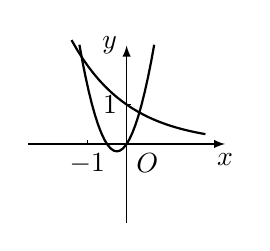
\begin{tikzpicture}[scale = 0.5, >=latex]
    \draw [->] (-2.5,0) -- (2.5,0) node [below] {$x$};
    \draw [->] (0,-2.) -- (0,2.5) node [left] {$y$};
    \draw (0,0) node [below right] {$O$};
    \draw (-1,0.1) -- (-1,0) node [below] {$-1$};
    \draw (0.1,1) -- (0,1) node [left] {$1$};
    \draw [domain = -1.2:0.7,thick] plot (\x,{3*\x * (\x+0.5)});
    \draw [domain = -1.4:2,thick] plot (\x,{(0.5)^\x}); 
\end{tikzpicture}
}{
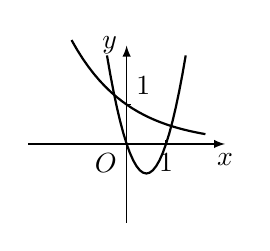
\begin{tikzpicture}[scale = 0.5, >=latex]
    \draw [->] (-2.5,0) -- (2.5,0) node [below] {$x$};
    \draw [->] (0,-2.) -- (0,2.5) node [left] {$y$};
    \draw (0,0) node [below left] {$O$};
    \draw (1,0.1) -- (1,0) node [below] {$1$};
    \draw (0.1,1) -- (0,1) node [above right] {$1$};
    \draw [domain = -0.5:1.5,thick] plot (\x,{3*\x*(\x-1)});
    \draw [domain = -1.4:2,thick] plot (\x,{(0.5)^\x}); 
\end{tikzpicture}
}{
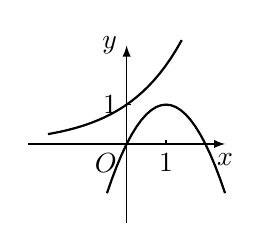
\begin{tikzpicture}[scale = 0.5, >=latex]
    \draw [->] (-2.5,0) -- (2.5,0) node [below] {$x$};
    \draw [->] (0,-2.) -- (0,2.5) node [left] {$y$};
    \draw (0,0) node [below left] {$O$};
    \draw (1,0.1) -- (1,0) node [below] {$1$};
    \draw (0.1,1) -- (0,1) node [left] {$1$};
    \draw [domain = -0.5:2.5,thick] plot ({\x},{-\x*(\x-2)});
    \draw [domain = -1.4:2,thick] plot ({-\x},{(0.5)^\x}); 
\end{tikzpicture}
}{
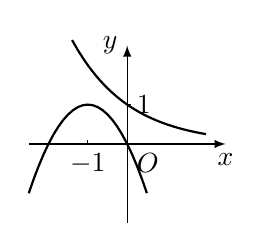
\begin{tikzpicture}[scale = 0.5, >=latex]
    \draw [->] (-2.5,0) -- (2.5,0) node [below] {$x$};
    \draw [->] (0,-2.) -- (0,2.5) node [left] {$y$};
    \draw (0,0) node [below right] {$O$};
    \draw (-1,0.1) -- (-1,0) node [below] {$-1$};
    \draw (0.1,1) -- (0,1) node [right] {$1$};
    \draw [domain = -2.5:0.5,thick] plot ({\x},{-\x*(\x+2)});
    \draw [domain = -1.4:2,thick] plot ({\x},{(0.5)^\x}); 
\end{tikzpicture}   
}
\item 设$a$为常数且$0<a<1$, 若$y=(\log_a \dfrac 35)^x$在$\mathbf{R}$上是严格增函数, 求实数$a$的取值范围.
\item 在同一平面直角坐标系中, 作出函数$y=(\dfrac 12)^x$及$y=x^{\frac 12}$的大致图像, 并求方程$(\dfrac 12)^x=x^{\frac 12}$的解的个数.
\item 已知集合$A=\{y|y=(\dfrac 12)^x,\  x\in [-2, 0)\}$, 用列举法表示集合$B=\{y|y=\log_3x,\  x\in A\text{且}y\in \mathbf{Z}\}$.
\item $\log_23$是有理数吗? 请证明你的结论.
\item 仅利用对数函数的单调性和计算器上的乘方功能来确定对数$\log_23$第二位小数的值.
\item 求函数$y=\dfrac1{2-x}+\sqrt{x^2-1}$的定义域.
\item 判断下列函数$y=f(x)$的奇偶性, 并说明理由:\\
(1) $f(x)=|\dfrac 12 x-3|+|\dfrac 12 x+3|$;\\
(2) $f(x)=x^3+\dfrac 2x$;\\
(3) $f(x)=x^2$, $x\in (k, 2)$(其中常数$k<2$).
\item 已知$m$、$n$是常数, 而函数$y=(m-1)x^2+3x+(2-n)$为奇函数. 求$m$、$n$的值.
\item 求函数$y=x+\dfrac 4x$的单调区间.
\item 分别作出下列函数的大致图像, 并指出它们的单调区间:\\
(1) $y=|x^2-4x|$;\\
(2) $y=2|x|-3$.
\item 已知二次函数$y=f(x)$, 其中$f(x)=ax^2-2ax+3-a \ (a>0)$. 比较$f(-1)$和$f(2)$的大小.
\item 已知$k$是常数, 设$\alpha$、$\beta$是二次方程$x^2-2kx+k+20=0$的两个实根. 问: 当$k$为
何值时, $(\alpha+1)^2+(\beta+1)^2$取到最小值?
\item 邮局规定: 当邮件质量不超过$100$g时, 每$20$g邮费$0.8$元, 且不足$20$g时按$20$g计算; 超过$100$g时, 超过$100$g的部分按每$100$g邮费$2$元计算, 且不足$100$g按$100$g
计算; 同时规定邮件总质量不得超过$2000$g. 请写出邮费关于邮件质量的函数表达式, 并计算$50$g和$500$g的邮件分别收多少邮费.
\item 若函数$y=(a^2+4a-5)x^2-4(a-1)x+3$的图像都在$x$轴上方(不含$x$轴), 求实数$a$的取值范围.
\item 已知$y=f(x)$是奇函数, 其定义域为$\mathbf{R}$; 而$y=g(x)$是偶函数, 其定义域为$D$. 判断函数$y=f(x)g(x)$的奇偶性, 并说明理由.
\item 设函数$y=x^2+10x-a+3$, 当$x\in [-2, +\infty)$时, 其函数值恒大于等于零. 求实数$a$的取值范围.
\item 已知函数$y=-x^2+2ax+1-a$, $x\in [0, 1]$的最大值为$2$. 求实数$a$的值.
\item 设$f(x)=x^2+ax+1$. 若对任意给定的实数$x$, $f(2+x)=f(2-x)$恒成立, 求实数$a$的值.
\item 已知$y=f(x)$是定义在$(-1, 1)$上的奇函数, 在区间$[0, 1)$上是严格减函数, 且$f(1-a)+f(1-a^2)<0$, 求实数$a$的取值范围.
\item 已知$f(x)=2-x^2$及$g(x)=x$. 定义$h(x)$如下: 当$f(x)\ge g(x)$时, $h(x)=g(x)$; 而当$f(x)<g(x)$时, $h(x)=f(x)$. 求函数$y=h(x)$的最大值.
\item 试讨论函数$y=\dfrac{x}{1-x^2}$的单调性.
\item 作出函数$y=(x^2-1)^2-1$的大致图像, 写出它的单调区间, 并证明你的结论.
\item 已知函数$y=f(x)$为偶函数, $y=g(x)$为奇函数, 且$f(x)+g(x)=x^2+2|x-1|+3$. 求$y=f(x)$及$y=g(x)$的表达式.
\item 设函数$y=f(x)$, $x\in \mathbf{R}$的反函数是$y=f^{-1}(x)$.\\
(1) 如果$y=f(x)$是奇函数, 那么$y=f^{-1}(x)$的奇偶性如何?\\
(2) 如果$y=f(x)$在定义域上是严格增函数, 那么$y=f^{-1}(x)$的单调性如何?
\item 选择题:\\
(1) 与$\sin(\theta -\dfrac\pi 2)$一定相等的是\bracket{20}.
\fourch{$\sin(\dfrac{3\pi}2-\theta)$}{$\cos(\theta -\dfrac{\pi}2)$}{$\cos (2\pi -\theta)$}{$\sin (\theta +\dfrac\pi 2)$}
(2) 当$0<\alpha<\dfrac\pi 4$时, 化简$\sqrt{1-\sin 2\alpha}$的结果是\bracket{20}.
\fourch{$\cos \alpha$}{$\sin \alpha-\cos \alpha$}{$\cos\alpha-\sin\alpha$}{$\sin\alpha+\cos\alpha$}
\item 填空题:\\
(1) 若$\theta$为锐角, 则$\log_{\sin \theta} (1+\cot^2\theta)=$\blank{50};\\
(2) 若$-\dfrac\pi 2<\alpha<0$, 则点$(\cot \alpha, \cos \alpha)$必在第\blank{50}象限;\\
(3) 若$\sin (\pi -\alpha)=\dfrac 23$, $\alpha\in (\dfrac\pi 2, \pi)$, 则$\sin 2\alpha=$\blank{50}.
\item 已知圆$O$上的一段圆弧长等于该圆的内接正方形的边长, 求这段圆弧所对的圆心角的弧度.
\item 已知角$\alpha$的终边经过点$P(3a, 4a)$($a\ne 0$), 求$\sin \alpha$、$\cos \alpha$和$\tan \alpha$.
\item 化简:\\
(1) $\dfrac{\sin (\theta -5\pi )}{\tan (3\pi -\theta )}\cdot \dfrac{\cot (\dfrac\pi 2-\theta )}{\tan (\theta -\dfrac{3\pi} 2)}\cdot \dfrac{\cos (8\pi -\theta )}{\sin(-\theta-4\pi)}$;\\
(2) $\sin (\theta -\dfrac\pi 4)+\cos (\theta +\dfrac\pi 4)$.
\item 已知$\tan \alpha=3$, 求$\dfrac 1{\sin^2\alpha+2\sin \alpha\cos \alpha}$的值.
\item 在$\triangle ABC$中, 已知$a=5$, $b=4$, $A=2B$. 求$\cos B$.
\item 已知$\triangle ABC$的面积为$S$, 求证:\\
(1) $S=\dfrac{a^2\sin B\sin C}{2\sin (B+C)}$;\\
(2) $S=\dfrac{a^2}{2(\cot B+\cot C)}$.
\item (1) 已知$\sin \alpha=\dfrac{\sqrt 5}5$, $\sin \beta=\dfrac{\sqrt {10}}{10}$, 且$\alpha$及$\beta$都是锐角. 求$\alpha+\beta$的值;\\
(2) 在$\triangle ABC$中, 已知$\tan A$与$\tan B$是方程$x^2-6x+7=0$的两个根, 求$\tan C$.
\item 证明: $(\sin \alpha+\sin \beta)^2+(\cos \alpha+\cos \beta)^2=4\cos^2\dfrac{\alpha-\beta}{2}$.
\item 选择题:\\
(1) 若$0<x<\dfrac\pi 4$, 且$\lg (\sin x+\cos x)=\dfrac12(3\lg 2-\lg 5)$, 则$\cos x-\sin x$的值为\bracket{20}.
\fourch{$\dfrac{\sqrt{6}}3$}{$\dfrac{\sqrt{3}}2$}{$\dfrac{\sqrt{10}}5$}{$\dfrac{\sqrt{5}}4$}
(2) 下列命题中, 真命题为\bracket{20}.
\onech{若点$P(a, 2a)$($a\ne 0$)为角$\alpha$的终边上一点, 则$\sin \alpha=\dfrac{2\sqrt 5}5$}
{同时满足$\sin \alpha=\dfrac 12$, $\cos \alpha=\dfrac{\sqrt3}2$的角$\alpha$有且只有一个}
{如果角$\alpha$满足$-3\pi <\alpha<-\dfrac 52\pi$, 那么角$\alpha$是第二象限的角}
{$\tan x=-\sqrt 3$的解集为$\{x|x=k\pi -\dfrac\pi 3, \  k\in \mathbf{Z}\}$}
\item 填空题:\\
(1) 在$\triangle ABC$中, 若$a^2+b^2+ab=c^2$, 则$C=$\blank{50};\\
(2) 若$\sin \theta =a$, $\cos \theta =-2a$, 且$\theta$为第四象限的角, 则实数$a=$\blank{50}.\\
\item 已知$\sin \alpha=a\sin \beta$, $b\cos \alpha=a\cos \beta$, 且$\alpha$及$\beta$均为锐角, 求证: $\cos \alpha= \sqrt{\dfrac{a^2-1}{b^2-1}}$.
\item 已知$0<\alpha<\dfrac\pi 2<\beta<\pi$, 且$\cos \beta=-\dfrac13$, $\sin (\alpha+\beta)=\dfrac79$, 求$\sin \alpha$的值.
\item 已知$\pi <\alpha<\dfrac{3\pi} 2$, $\pi <\beta<\dfrac{3\pi} 2$, 且$\sin \alpha=-\dfrac{\sqrt 5}5$, $\cos \beta=-\dfrac{\sqrt{10}}{10}$. 求$\alpha-\beta$的值.
\item 已知$(1+\tan \alpha)(1+\tan \beta)=2$, 且$\alpha$及$\beta$都是锐角. 求证: $\alpha+\beta=\dfrac{\pi}{4}$.
\item 已知$\alpha$是第二象限的角, 且$\sin \alpha=\dfrac{\sqrt {15}}4$. 求$\dfrac{\sin (\alpha+\dfrac{\pi}{4})}{1+\sin 2\alpha+\cos 2\alpha}$的值.
\item 证明:\\
(1) $\dfrac{2(1+\sin 2\alpha)}{1+\sin 2\alpha+\cos 2\alpha}=1+\tan \alpha$;\\
(2) $2\sin \alpha+\sin 2\alpha=\dfrac{2\sin^3\alpha}{1-\cos \alpha}$.
\item 根据下列条件, 分别判断三角形$ABC$的形状:\\
(1) $\sin C+\sin (B-A)=\sin 2A$;\\
(2) $\dfrac{\tan A}{\tan B}=\dfrac{a^2}{b^2}$.
\item 在$\triangle ABC$中, 求证: $\tan \dfrac A2\tan \dfrac B2+\tan \dfrac B2\tan\dfrac C2+\tan\dfrac C2\tan\dfrac A2=1$.
\item (1) 完成下表($\theta$为弧度数):
\begin{center}
\begin{tabular}{|c|p{.15\textwidth}<{\centering}|p{.15\textwidth}<{\centering}|p{.15\textwidth}<{\centering}|p{.15\textwidth}<{\centering}|p{.15\textwidth}<{\centering}|}
    \hline
    $\theta$ & $1$ & $0.5$ & $0.1$ & $0.01$ & $0.001$\\ \hline
    $\sin\theta$ & & & & &\\ \hline
    $\dfrac{\sin\theta}{\theta}$ & & & & &\\ \hline
\end{tabular}
\end{center}
(2) 观察上表中的数据, 你能发现什么规律?\\
(3) 已知$0<\theta <\dfrac \pi 2$, 利用图形面积公式证明$\sin \theta <\theta <\tan \theta$, 并应用该公式说明(2)中猜想的合理性.
\item 在$\triangle ABC$中, 已知$A=30^\circ$, $b=18$. 分别根据下列条件求$B$:\\
(1) \textcircled{1} $a=6$, \textcircled{2} $a=9$, \textcircled{3} $a=13$, \textcircled{4} $a=18$, \textcircled{5} $a=22$;\\
(2) 根据上述计算结果, 讨论使$B$有一解、两解或无解时$a$的取值情况.
\item (1) 根据$\cos 54^\circ=\sin 36^\circ$和三倍角公式, 求$\sin 18^\circ$的值;\\
(2) 你还能使用其他方法求$\sin 18^\circ$的值吗? 若能, 请给出你的求法.
\item 如图, 要在$A$和$D$两地之间修建一条笔直的隧道, 现在从$B$地和$C$地测量得到: $\angle DBC=24.2^\circ$, $\angle DCB=35.4^\circ$, $\angle DBA=31.6^\circ$, $\angle DCA=17.5^\circ$. 试求$\angle DAB$以确定隧道$AD$的方向(结果精确到$0.1^\circ$).
\begin{center}
    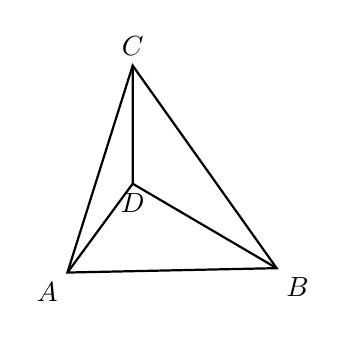
\begin{tikzpicture}
        \draw (0,0) node [below] {$D$} coordinate (D) (0,1.5) node [above] {$C$} coordinate (C) (-0.8287,-1.12831) node [below left] {$A$} coordinate (A) (1.82829,-1.07265) node [below right] {$B$} coordinate (B);
        \draw [thick] (A) -- (B) -- (C) -- cycle;
        \draw [thick] (D) -- (A) (D) -- (B) (D) -- (C);
    \end{tikzpicture}
\end{center}
\item 求下列函数的最小正周期:\\
(1) $y=\sin \dfrac x2$;\\
(2) $y=2\cos (3x-\dfrac \pi 4)$.
\item 判断下列函数的奇偶性, 并说明理由:\\
(1) $y=\sin |2x|$;\\
(2) $y=\tan 5x$;\\
(3) $y= \dfrac1 {\cos x}$;\\
(4) $y=\sin (x+\dfrac\pi 6)$.
\item 已知$2\sin (2x)=\sqrt 3, \ x\in (-\dfrac \pi 4, \dfrac\pi 4)$. 求$x$的值.
\item 求下列函数的单调区间:\\
(1) $y=-\sin 2x$;\\
(2) $y=2\sin (x+\dfrac\pi 3)$;\\
(3) $y=\cos (\dfrac x2-\dfrac \pi 4)$;\\
(4) $y=2\tan (2x+\dfrac \pi 4)$.
\item 作出函数$y=2\sin (2x+\dfrac \pi 3)$的大致图像.
\item 已知函数$y=A\sin (\omega x+\varphi) \ (A>0, \ \omega>0)$的振幅是$3$, 最小正周期是$\dfrac{2\pi} 3$, 初始相位是$\dfrac\pi 6$. 求这个函数的表达式.
\item 求下列函数的最大值和最小值, 并求出取得最大值和最小值时所有$x$的值:\\
(1) $y=\cos^2x+\cos x-2$;\\
(2) $y=\sin 2x, \ x\in [ -\dfrac{2\pi} 3, \dfrac \pi 3]$;\\
(3) $y=\sin^22x-2\sin 2x$;\\
(4) $y=\cos (x-\dfrac\pi 6),\  x\in  [-\dfrac\pi 6, \dfrac\pi 4]$.
\item 某实验室一天的温度$y$(单位:$^\circ\text{C}$)随时间$t$(单位:$\text{h}$)的变化近似满足函数关系$y=10-\sqrt 3\cos\dfrac \pi {12}t-\sin \dfrac\pi {12} t, \ t\in [0, 24)$.\\
(1) 求实验室一天中的最大温差;\\
(2) 若要求实验室温度不高于$11^\circ\text{C}$, 则在哪段时间实验室需要降温?
\item 求函数$y=\sin (2x-\dfrac \pi 4)-2\sqrt 2\sin^2x$的最小正周期.
\item 在$(0, 2\pi )$内, 求使$\sin x>\cos x$成立的$x$的取值范围.
\item 求下列函数的最大值, 并求出取得最大值时所有$x$的值:\\
(1) $y=2\sin^2x+\sin 2x-1$;\\
(2) $y=1-\sin x-2\cos^2x, \  x\in  [\dfrac \pi 3, \dfrac{4\pi} 3]$.
\item 若函数$y=2\sin \omega x$(其中常数$\omega$是小于$1$的正数)在区间$[0, \dfrac\pi 3]$上的最大值是$\sqrt 2$, 求$\omega$的值.
\item 如图, 摩天轮上一点$P$距离地面的高度$y$关于时间$t$的函数表达式为$y=A\sin (\omega t+\varphi)+b$, $\varphi\in [-\pi , \pi]$. 已知摩天轮
的半径为$50\text{m}$, 其中心点$O$距地面$60\text{m}$, 摩天轮以每$30$分钟转一圈的方式做匀速转动, 而点$P$的起始位置在摩天轮的最低
点处.
\begin{center}
    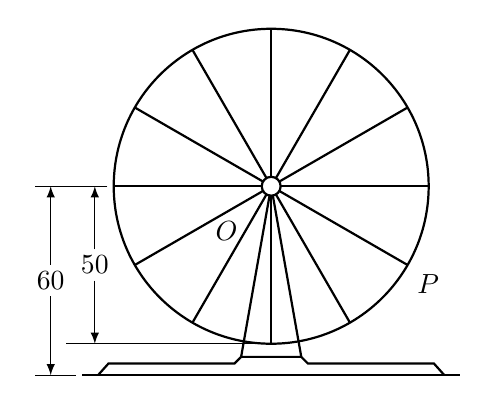
\begin{tikzpicture}[>=latex,scale = 0.4]
        \draw [thick] (0,0) circle (0.3) (0,0) circle (5);
        \foreach \i in {0,30,...,330}{\draw [thick] (\i:0.3) -- (\i:5);};
        \draw [thick] (-80:0.3) -- (-80:5.5) coordinate (R) (-100:0.3) -- (-100:5.5) coordinate (L) (L) -- (R);
        \draw [thick] (L) --++ (-135:0.3) --++ (-4,0) -- (-5.5,-6) (R) --++ (-45:0.3) --++ (4,0) -- (5.5,-6); 
        \draw [thick] (-6,-6) -- (6,-6);
        \draw (-6.2,-6) -- (-7.5,-6) (-5.2,0) -- (-7.5,0) (0,-5) -- (-6.5,-5);
        \draw [->] (-5.6,-2) -- (-5.6,0);
        \draw [->] (-5.6,-3) -- (-5.6,-5);
        \draw (-5.6,-2.5) node {$50$};
        \draw [->] (-7,-2.5) -- (-7,0);
        \draw [->] (-7,-3.5) -- (-7,-6);
        \draw (-7,-3) node {$60$};
        \draw (225:2) node {$O$};
        \draw (-30:5) node [below right] {$P$};
    \end{tikzpicture}
\end{center}
(1) 根据条件具体写出$y$($\text{m}$)关于$t$($\text{min}$)的函数表达式;\\
(2) 在摩天轮转动的一圈内, 点$P$有多长时间距离地面超过$85\text{m}$?
\item 说明: 用上一章6.3节给出的记号$\arcsin$与$\arccos$(见必修第二册教材第45页), 可以定义函数$y=\arcsin x \ (x\in [0, 1])$与$y=\arccos x \ (x\in [0, 1])$.\\
验证:\\
(1) 函数$y=\sin x\ (x\in [0, \dfrac\pi 2])$与函数$y=\arcsin x \ (x\in [0, 1])$互为反函数;\\
(2) 函数$y=\cos x \ (x\in [0, \dfrac \pi 2])$与函数$y=\arccos x\ (x\in [0, 1])$互为反函数.
\item 把上题的记号略作推广: 对实数$x\in [-1, 1]$, 若实数$y\in [-\dfrac \pi 2, \dfrac\pi 2]$使得$\sin y=x$, 则记$y=\arcsin x$; 类似地, 对实数$x\in [-1, 1]$, 若实数$y\in [0, \pi]$使得$\cos y=x$, 则记$y=\arccos x$. 说明: 经过推广的记号$\arcsin$与$\arccos$, 定义了函数$y=\arcsin x \ (x\in [-1, 1])$与$y=\arccos x \ (x\in [-1, 1])$.\\
验证:
(1) 函数$y=\sin x \ (x\in  [-\dfrac\pi 2, \dfrac\pi 2])$与函数$y=\arcsin x \ (x\in [-1, 1])$互为反函数;\\
(2) 函数$y=\cos x\ (x\in [0, \pi])$与函数$y=\arccos x \ (x\in [-1, 1])$互为反函数.
\item 对$y=\tan x$与$y=\arctan x$做类似的工作.
\item 定义在区间$(0, \dfrac\pi 2)$上的函数$y=6\cos x$的图像与$y=5\tan x$的图像的交点为$P$, 过点$P$作垂直于$x$轴的垂线$PP_1$, 其垂足为$P_1$. 设直线$PP_1$与$y=\sin x$的图像交于点$P_2$, 求线段$P_1P_2$的长.
\item 已知定义在$\mathbf{R}$上的偶函数$y=f(x)$的最小正周期为$2$, 当$0\le x\le 1$时, $f(x)=x$.\\
(1) 求当$5\le x\le 6$时函数$y=f(x)$的表达式;\\
(2) 若函数$y=kx,\ x\in \mathbf{R}$与函数$y=f(x)$的图像恰有$7$个不同的交点, 求$k$的值.
\item 如图, 有一块边长为$3\text{m}$的正方形铁皮$ABCD$, 其中阴影部分$ATN$是一个半径为$2\text{m}$的扇形. 设这个扇形已经腐蚀不能
使用, 但其余部分均完好. 工人师傅想在未被腐蚀的部分截下一块其边落在$BC$与$CD$上的矩形铁皮$PQCR$, 使点$P$在弧$TN$上. 设$\angle TAP=\theta$, 矩形$PQCR$的面积为$S\text{m}^2$.
\begin{center}
    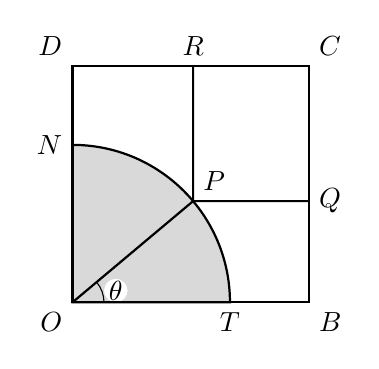
\begin{tikzpicture}
        \begin{scope}[even odd rule]
            \clip (0,0) rectangle (3,3) (0.55,0.15) circle (0.15);
            \fill [gray!30] (0,0) -- (2,0) arc (0:90:2) -- cycle;
        \end{scope}

        \draw [thick] (0,0) node [below left] {$O$} -- (3,0) node [below right] {$B$} -- (3,3) node [above right] {$C$} -- (0,3) node [above left] {$D$} -- cycle;
        \draw [thick] (0,0) -- (40:2) node [above right] {$P$} -- (3,{2*sin(40)}) node [right] {$Q$} (40:2) -- ({2*cos(40)},3) node [above] {$R$};
        \draw [thick] (0,0) -- (2,0) node [below] {$T$} arc (0:90:2) node [left] {$N$} -- cycle;
        \draw (0.4,0) arc (0:40:0.4) (0.55,0.15) node {$\theta$};
    \end{tikzpicture}
\end{center}
(1) 求$S$关于$\theta$的函数表达式;\\
(2) 求$S$的最大值及$S$取得最大值时$\theta$的值.
\item 如图, 在边长为$1$的小正方形组成的网格上, 求:
\begin{center}
    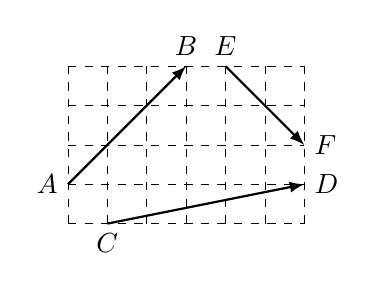
\begin{tikzpicture}[>=latex,scale = 0.5]
        \foreach \i in {0,1,...,4} {\draw [dashed, very thin] (0,\i) -- (6,\i);};
        \foreach \i in {0,1,...,6} {\draw [dashed, very thin] (\i,0) -- (\i,4);};
        \draw [thick,->] (0,1) node [left] {$A$} -- (3,4) node [above] {$B$};
        \draw [thick,->] (1,0) node [below] {$C$} -- (6,1) node [right] {$D$};
        \draw [thick, ->] (4,4) node [above] {$E$} -- (6,2) node [right] {$F$};       
    \end{tikzpicture}
\end{center}
(1) $|\overrightarrow{AB}|$;\\
(2) $|\overrightarrow{CD}|$;\\
(3) $|\overrightarrow{EF}|$.
\item 已知$\overrightarrow a$、$\overrightarrow b$均为非零向量, 写出$|\overrightarrow a+\overrightarrow b|=|\overrightarrow a|+|\overrightarrow b|$成立的充要条件.
\item 已知$\overrightarrow a$、$\overrightarrow b$为非零向量, 且$\overrightarrow a$、$\overrightarrow b$、$5\overrightarrow a-4\overrightarrow b$在同一起点上. 求证: 它们的终点在同一条直线上.
\item 在矩形$ABCD$中, 边$AB$、$AD$的长分别为$2$、$1$, 若$M$、$N$分别是边$BC$、$CD$上的点, 且满足$\dfrac{|\overrightarrow{BM}|}{|\overrightarrow{BC}|}=\dfrac{|\overrightarrow{CN}|}{|\overrightarrow{CD}|}$, 则$\overrightarrow{AM}\cdot \overrightarrow{AN}$的取值范围是\blank{50}.
\item 已知两个向量$\overrightarrow {e_1}$、$\overrightarrow {e_2}$满足$|\overrightarrow {e_1}|=2$, $|\overrightarrow {e_2}|=1$, $\langle \overrightarrow {e_1}, \overrightarrow {e_2}\rangle=60^\circ$, 且向量$2\lambda \overrightarrow {e_1}+7\overrightarrow {e_2}$与向量$\overrightarrow {e_1}+\lambda \overrightarrow {e_2}$的夹角为钝角. 求实数$\lambda$的取值范围.
\item 已知向量$\overrightarrow a=(1, 0)$, $\overrightarrow b=(2, 1)$.\\
(1) 求$|\overrightarrow a+3\overrightarrow b|$;\\
(2) 当$k$为何实数时, $k\overrightarrow a-\overrightarrow b$与$\overrightarrow a+3\overrightarrow b$平行? 平行时它们是同向还是反向?
\item 已知在平面直角坐标系中, $O$为原点, 点$A(4, -3)$, $B(-5, 12)$.\\
(1) 求向量$\overrightarrow{AB}$的坐标及$|\overrightarrow{AB}|$;\\
(2) 已知向量$\overrightarrow{OC}=2\overrightarrow{OA}+\overrightarrow{OB}$, $\overrightarrow{OD}=\overrightarrow{OA}-3\overrightarrow{OB}$, 求$\overrightarrow{OC}$及$\overrightarrow{OD}$的坐标;\\
(3) 求$\overrightarrow{OA}\cdot\overrightarrow{OB}$.
\item 已知向量$\overrightarrow a=(3, -2)$, $\overrightarrow b=(-2, 1)$, $\overrightarrow c=(7, -4)$, 求$\lambda,\mu$, 使得$\overrightarrow c=\lambda \overrightarrow a+\mu \overrightarrow b$.
\item 已知点$M(3, -2)$、$N(-5, -1)$, 且$\overrightarrow{MP}=\dfrac 13\overrightarrow{MN}$. 求点$P$的坐标.
\item 在等腰三角形$ABC$中, 已知$D$为底边$BC$的中点. 求证: $AD\perp BC$.
\item 如图, 在四边形$ABCD$中, $G$为对角线$AC$与$BD$中点连线$MN$的中点, $P$为平面上任意给定的一点. 求证: $4\overrightarrow{PG}=\overrightarrow{PA}+\overrightarrow{PB}+\overrightarrow{PC}+\overrightarrow{PD}$.
\item 在四边形$ABCD$中, 向量$\overrightarrow{AB}=\overrightarrow i+2\overrightarrow j$, $\overrightarrow{BC}=-4\overrightarrow i-\overrightarrow j$, $\overrightarrow{CD}=-5\overrightarrow i-3\overrightarrow j$. 求证: $ABCD$为梯形.
\begin{center}
    \begin{tikzpicture}
        \draw [thick] (0,0) node [below left] {$B$} coordinate (B) -- (2,0) node [below right] {$C$} coordinate (C) -- (2.4,2.5) node [above right] {$D$} coordinate (D) -- (-0.1,1.5) node [above left] {$A$} coordinate (A) -- cycle;
        \draw [thick] (A) -- (C) (B) -- (D);
        \filldraw ($(B)!0.5!(D)$) circle (0.03) node [above] {$M$} coordinate (M);
        \filldraw ($(A)!0.5!(C)$) circle (0.03) node [below] {$N$} coordinate (N);
        \filldraw ($(M)!0.5!(N)$) circle (0.03) node [right] {$G$} coordinate (G);
        \filldraw (3,1) circle (0.03) node [right] {$P$};
        \draw [thick] (M) -- (N);
    \end{tikzpicture}
\end{center}
\item 已知$\overrightarrow a$、$\overrightarrow b$、$\overrightarrow c$均为非零向量, 其中的任意两个向量都不平行, 且$\overrightarrow a+\overrightarrow b$与$\overrightarrow c$是平行向量, $\overrightarrow a+\overrightarrow c$与$\overrightarrow b$是平行向量. 求证: $\overrightarrow b+\overrightarrow c$与$\overrightarrow a$是平行向量.
\item 如图, 点$A$、$M$、$B$在同一条直线上, 点$O$不在该直线上, 且$\overrightarrow{AM}=\dfrac 13 \overrightarrow{AB}$. 设
$\overrightarrow{OA}=\overrightarrow a$, $\overrightarrow{OB}=\overrightarrow b$, $\overrightarrow{OM}=\overrightarrow c$, 试用向量$\overrightarrow a$、$\overrightarrow b$表示$\overrightarrow c$.
\begin{center}
    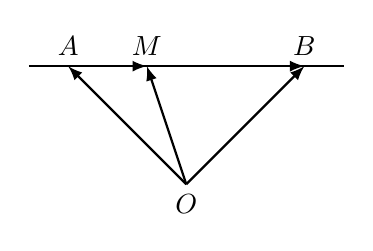
\begin{tikzpicture}[>=latex]
        \draw [thick] (-0.5,0) -- (3.5,0);
        \draw [->,thick] (1.5,-1.5) node [below] {$O$}-- (0,0) node [above] {$A$};
        \draw [->,thick] (1.5,-1.5) -- (3,0);
        \draw [->,thick] (1.5,-1.5) -- (1,0);
        \draw [->,thick] (0,0) -- (1,0) node [above] {$M$};
        \draw [->,thick] (1,0) -- (3,0) node [above] {$B$};
    \end{tikzpicture}
\end{center}
\item 设平面上有两个向量$\overrightarrow a=(\cos \alpha, \sin \alpha)  (0^\circ\le \alpha<360^\circ)$, $\overrightarrow b=(-\dfrac 12, \dfrac{\sqrt 3}2)$.\\
(1) 求证: 向量$\overrightarrow a+\overrightarrow b$与$\overrightarrow a-\overrightarrow b$垂直;\\
(2) 当向量$\sqrt 3\overrightarrow a+\overrightarrow b$与$\overrightarrow a-\sqrt 3\overrightarrow b$的模相等时, 求$\alpha$的大小.
\item 如图, 在矩形$ABCD$中, $AB=\sqrt 2$, $BC=2$, $E$为$BC$的中点, 点$F$在边$CD$上且$\overrightarrow{AB}\cdot \overrightarrow{AF}=\sqrt{2}$. 求$\overrightarrow{AE}\cdot \overrightarrow{BF}$的值.
\begin{center}
    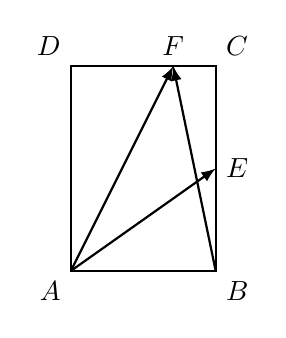
\begin{tikzpicture}[>=latex,thick,scale = 1.3]
        \draw (0,0) node [below left] {$A$} rectangle ({sqrt(2)},2) node [above right] {$C$};
        \draw [->,thick] (0,0) -- ({sqrt(2)},1) node [right] {$E$};
        \draw [->] (0,0) -- (1,2) node [above] {$F$};
        \draw [->] ({sqrt(2)},0) node [below right] {$B$} -- (1,2);
        \draw (0,2) node [above left] {$D$};
    \end{tikzpicture}
\end{center}
\item 已知等边三角形$AB$C的边长为$1$, $\overrightarrow{BC}=\overrightarrow a$, $\overrightarrow{CA}=\overrightarrow b$, $\overrightarrow{AB}=\overrightarrow c$. 求$\overrightarrow a\cdot \overrightarrow b+\overrightarrow b\cdot \overrightarrow c+\overrightarrow c\cdot \overrightarrow a$.
\item 已知向量$\overrightarrow{OA}=(k, 12)$, $\overrightarrow{OB}=(4, 5)$, $\overrightarrow{OC}=(-k, 10)$, 且$A$、$B$、$C$三点共线. 求实数$k$的值.
\item 已知向量$\overrightarrow{OA}=(1, 7)$, $\overrightarrow{OB}=(5, 1)$, $\overrightarrow{OP}=(2, 1)$, $K$为直线$OP$上的一个动点, 当$\overrightarrow{KA}\cdot\overrightarrow{KB}$取最小值时, 求向量$\overrightarrow{OK}$的坐标.
\item 如图, 在正方形$ABCD$中, $P$是对角线$AC$上一点, $PE$垂直$AB$于点$E$, $PF$垂直$BC$于点$F$. 求证: $PD\perp EF$.
\begin{center}
    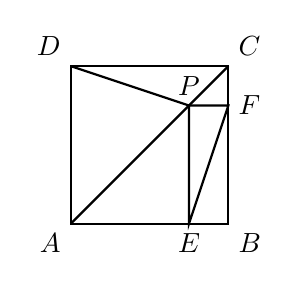
\begin{tikzpicture}[thick]
        \draw (0,0) node [below left] {$A$} rectangle (2,2) node [above right] {$C$};
        \draw (0,2) node [above left] {$D$} -- (1.5,1.5) node [above] {$P$};
        \draw (1.5,1.5) -- (1.5,0) node [below] {$E$} -- (2,1.5) node [right] {$F$} -- cycle;
        \draw (2,0) node [below right] {$B$};
        \draw (0,0) -- (2,2);
    \end{tikzpicture}
\end{center}
\item 证明: 三角形的三条高相交于一点.
\item 如图, 甲、乙分处河的两岸, 欲拉船$M$逆流而上, 需在正前方有$3000\text{N}$的力. 已知甲所用的力$\overrightarrow{f_1}$的大小为$2000\text{N}$, 且与$M$的前进方向的夹角为$\dfrac\pi 6$, 求乙所用的力$\overrightarrow{f_2}$.
\begin{center}
    \begin{tikzpicture}[thick,>=latex,scale = 1.5]
        \fill [fill = gray!20] (0,0.3) -- (0,1.4) -- (3,1.7) -- (3,0.6) -- cycle;
        \draw (0,1.4) -- (3,1.7) (0,0.3) -- (3,0.6);
        \draw [->] (0.6,1) node [below left] {$M$} -- (3,1);
        \draw [dashed,thin] (0,1) -- (0.6,1);
        \draw [->] (0.6,1) --++ (30:1.6) node [above right] {$\overrightarrow{f_1}$};
        \draw [->] (0.6,1) --++ ({2.4-1.6*cos(30)},{-1.6*sin(30)}) node [below right] {$\overrightarrow{f_2}$};
        \draw (2.2,1) node [above] {前进方向};
    \end{tikzpicture}
\end{center}
\item 在$\triangle ABC$中, $AB=AC=5$, $BC=6$, $M$是边$AC$上靠近$A$的一个三等分点. 问: 在线段$BM$上是否存在点$P$, 使得$PC\perp BM$?
\item 在$\triangle ABC$中, 已知点$O$、$G$、$H$分别是三角形的外心、重心和垂心. 求证: $O$、$G$、$H$三点共线(此直线称为欧拉线).
\item 选择题:\\
(1) 虚数的平方一定是\bracket{20}.
\fourch{正实数}{负实数}{虚数}{虚数或负实数}
(2) 如果复平面上的向量$\overrightarrow{AB}$所对应的复数是$-3+2\mathrm{i}$, 那么向量$\overrightarrow{BA}$所对应的复数是\bracket{20}.
\fourch{$3-2\mathrm{i}$}{$3+2\mathrm{i}$}{$-3+2\mathrm{i}$}{$-3-2\mathrm{i}$}
\item 填空题:\\
(1) 设$z=11-60\mathrm{i}$, 则$\mathrm{Re}z=$\blank{50}; $\mathrm{Im}z=$\blank{50}; $|z|=$\blank{50}; $\overline{z}=$\blank{50}.\\
(2) 下列三个命题中, 真命题是\blank{50}.\\
\textcircled{1} 在复平面上, 表示实数的点都在实轴上, 表示虚数的点都在虚轴上;\\
\textcircled{2} 任何一个表示虚数的点一定在某一个象限内;\\
\textcircled{3} 复数的模表示该复数在复平面上所对应的点到原点的距离.
\item 已知复数$z=(a^2-2a-3)+(a^2-4a+3)\mathrm{i}$, 其中$a$是实数.\\
(1) 若$z\in \mathbf{R}$, 求$a$的值;\\
(2) 若$z$在复平面上所对应的点位于第一象限, 求$a$的取值范围.
\item 已知复数$z_1=(a^2-a-6)+(1-2a)\mathrm{i}$, $z_2=(a-3)+(a^2-2a+2)\mathrm{i}$, 其中$a\in \mathbf{R}$.
若$\overline{z_1}=z_2$, 求$a$的值.
\item 计算:\\
(1) $(4+\mathrm{i})(3+2\mathrm{i})$;\\
(2) $(\sqrt 2+\sqrt 3\mathrm{i})(\sqrt 2-\sqrt 3\mathrm{i})(-\sqrt 3+\sqrt 2\mathrm{i})(-\sqrt 3-\sqrt 2\mathrm{i})$;\\
(3) $\dfrac{-3+29\mathrm{i}}{1+2\mathrm{i}}$;\\
(4) $\dfrac{(1+\mathrm{i})^4}{1+2\mathrm{i}}+\dfrac{(1-\mathrm{i})^4}{1-2\mathrm{i}}$;\\
(5) $[(\sqrt 3+1)+(\sqrt 3-1)\mathrm{i}]^2$.
\item 已知复数$z=\dfrac{(-3-\mathrm{\mathrm{i}})^2(2-\mathrm{\mathrm{i}})}{(1+2\mathrm{i})^3}$, 求$|z|$.
\item 在复数范围内解下列方程:\\
(1) $x^2-4x+8=0$;\\
(2) $3x^2+2x-3=0$.
\item 选择题:\\
(1) 设$z_1$、$z_2\in \mathbf{C}$, 则``$|z_1|=|z_2|$''是``$z_1=z_2$''的\bracket{20}.
\twoch{充分非必要条件}{必要非充分条件}{充要条件}{既非充分也非必要条件}\\
(2)设复数$z=a+b\mathrm{i}$($a,b\in \mathbf{R}$), 则$z^2$是纯虚数的充要条件是\bracket{20}.
\fourch{$a^2=b^2$}{$a^2+b^2=0$}{$|a|=|b|\ne 0$}{$ab\ne 0$}
\item 若复数$z$满足$z+\overline{z}=2$, $(z-\overline{z})\mathrm{i}=2$, 求$|z|$.
\item 若复数$z_1$和复数$z_2$满足$z_1z_2=3-4\mathrm{i}$, $|z_1|=2$, 求$|z_2|$.
\item 若$x_1$和$x_2$是方程$x^2-5x+8=0$的两个根, 求$|x_1|+|x_2|$的值.
\item 若复数$z_1$和复数$z_2$满足$|z_1|=3$, $|z_2|=4$, $|z_1+z_2|=5$, 求$|z_1-z_2|$.
\item 已知复数$z_1$和复数$z_2$满足$z_1+z_2=3-5\mathrm{i}$, $\overline{z_1}-\overline{z_2}=-2+3\mathrm{i}$. 求$z_1^2-z_2^2$.
\item 如图, 在长方体$ABCD-A_1B_1C_1D_1$中, $E$为$A_1B_1$的中点, $AB=BB_1=2$, $AC=2\sqrt 5$. 求异面直线$BE$与$AC$所成角的
大小. 
\begin{center}
    \begin{tikzpicture}[thick]
        \draw (0,0) node [below left] {$A$} coordinate (A) --++ (2,0) node [below right] {$B$} coordinate (B) --++ (45:{2*sqrt(5)/2}) node [right] {$C$} coordinate (C)
        --++ (0,2) node [above right] {$C_1$} coordinate (C1)
        --++ (-2,0) node [above left] {$D_1$} coordinate (D1) --++ (225:{2*sqrt(5)/2}) node [left] {$A_1$} coordinate (A1) -- cycle;
        \draw (A) ++ (2,2) node [right] {$B_1$} coordinate (B1) -- (B) (B1) --++ (45:{2*sqrt(5)/2}) (B1) --++ (-2,0);
        \draw [dashed] (A) --++ (45:{2*sqrt(5)/2}) node [left] {$D$} coordinate (D) --++ (2,0) (D) --++ (0,2);
        \draw ($(A1)!0.5!(B1)$) node [above] {$E$} -- (B);
        \draw [dashed] (A) -- (C);
    \end{tikzpicture}
\end{center}
\item 如图, 设$P$为矩形$ABCD$所在平面外的一点, 矩形对角线的交点为$O$, $M$为$PB$的中点. 判断下列结论是否正确, 并说
明理由:\\
\begin{center}
    \begin{tikzpicture}[thick]
        \draw (0,0) node [below left] {$A$} coordinate (A) -- (3,0) node [below right] {$B$} coordinate (B)--++ (45:1.5) node [above right] {$C$} coordinate (C);
        \draw [dashed] (C) --++ (-3,0) node [above right] {$D$} coordinate (D) -- (A);
        \draw [dashed] (A) -- (C) (B) -- (D);
        \draw ($(A)!0.5!(C)$) node [below] {$O$} coordinate (O) ++ (0,3) node [above] {$P$} coordinate (P);
        \draw (P) -- (A) (P) -- (B) (P) -- (C);
        \draw ($(P)!0.5!(B)$) node [above right] {$M$} coordinate (M);
        \draw [dashed] (M) -- (O) (P) -- (D);
    \end{tikzpicture}
\end{center}
(1) $OM\parallel PD$;\\
(2) $OM\parallel\text{平面}PCD$;\\
(3) $OM\parallel\text{平面}PDA$;\\
(4) $OM\parallel\text{平面}PBA$;\\
(5) $OM\parallel\text{平面}PBC$.
\item 如图, 正方体的棱长是$a$, 点$E$、$F$分别是两条棱的中点.
\begin{center}
    \begin{tikzpicture}[thick]
        \path (0,0) node [below left] {$A$} coordinate (A) --++ (2.5,0) node [below right] {$B$} coordinate (B) --++ (45:{2.5/2}) node [right] {$C$} coordinate (C)
        --++ (0,2.5) node [above right] {$C_1$} coordinate (C1)
        --++ (-2.5,0) node [above left] {$D_1$} coordinate (D1) --++ (225:{2.5/2}) node [left] {$A_1$} coordinate (A1) -- cycle;
        \path (A) ++ (2.5,2.5) node [right] {$B_1$} coordinate (B1) -- (B) (B1) --++ (45:{2.5/2}) (B1) --++ (-2.5,0);
        \path [dashed] (A) --++ (45:{2.5/2}) node [left] {$D$} coordinate (D) --++ (2.5,0) (D) --++ (0,2.5);
        \draw ($(A1)!0.5!(D1)$) node [above left] {$E$} coordinate (E) ($(A1)!0.5!(B1)$) node [above] {$F$} coordinate (F);
        \fill [gray!30] (B) -- (D) -- (E) -- (F);
        \draw (B) -- (F) -- (E);
        \draw [dashed] (B) -- (D) -- (E) (D) -- (C) (D) -- (A) (D) -- (D1);
        \draw (A) -- (B) -- (C) -- (C1) -- (D1) -- (A1) -- (A) (B1) -- (A1) (B1) -- (C1) (B1) -- (B);
    \end{tikzpicture}
\end{center}
(1) 求证: 四边形$BDEF$(图中阴影部分)是一个梯形;\\
(2) 求四边形$BDEF$的面积.
\item 判断下列命题的真假, 并说明理由:\\
(1) 若直线$l$与平面$M$斜交, 则$M$内不存在与$l$垂直的直线;\\
(2) 若直线$l\perp\text{平面}M$, 则$M$内不存在与$l$不垂直的直线;\\
(3) 若直线$l$与平面$M$斜交, 则$M$内不存在与$l$平行的直线;\\
(4) 若直线$l\parallel\text{平面}M$, 则$M$内不存在与$l$不平行的直线.
\item 如果不在平面上的一条直线上有两点到这个平面的距离相等, 那么这条直线和这个平面有什么位置关系? 画示意图表示.
\item 如图, 直线$AA'$、$BB'$、$CC'$相交于点$O$, 且$AO=A'O$, $BO=B'O$, $CO=C'O$. 求证: $\text{平面}ABC\parallel \text{平面}A'B'C'$.
\begin{center}
    \begin{tikzpicture}[thick]
        \draw (0,0) node [below left] {$A$} coordinate (A);
        \draw (2.5,-0.5) node [below right] {$B$} coordinate (B);
        \draw (1.5,0.5) node [below] {$C$} coordinate (C);
        \draw (1,1.5) node [left] {$O$} coordinate (O);
        \draw (A) -- (B) -- (O) -- cycle;
        \draw [dashed] (A) -- (C) -- (B) (C) -- (O);
        \draw ($(O)!-1!(C)$) node [above] {$C'$} coordinate (C1);
        \draw ($(O)!-1!(A)$) node [right] {$A'$} coordinate (A1);
        \draw ($(O)!-1!(B)$) node [left] {$B'$} coordinate (B1);
        \draw (O) -- (A1) -- (B1) -- (C1) -- (O) (A1) -- (C1) (B1) -- (O);
    \end{tikzpicture}
\end{center}
\item 已知直线$l\perp\text{平面}\alpha$, 直线$m\subset\text{平面}\beta$, 判断下列命题的真假, 并说明理由:\\
(1) 若$\alpha\parallel \beta$, 则$l\perp m$;\\
(2) 若$\alpha\perp \beta$, 则$l\parallel m$;\\
(3) 若$l\parallel m$, 则$\alpha\perp \beta$;\\
(4) 若$l\perp m$, 则$\alpha\parallel \beta$.
\item 如图, 已知线段$AB$垂直于三角形$BCD$所在的平面, 且$AB=BC=CD=1$, $\angle BCD=90^\circ$. $BE\perp AD$, $E$为垂足, $F$为$AC$的中点. 求$EF$的长.
\begin{center}
    \begin{tikzpicture}[thick,scale = 2]
        \draw (0,0) node [left] {$B$} coordinate (B) -- (0,1) node [above left] {$A$} coordinate (A);
        \draw ({sqrt(2)/2},0) ++ (-45:{sqrt(2)/4}) coordinate (C) node [below] {$C$};
        \draw ({sqrt(2)},0) node [right] {$D$} coordinate (D) -- (C) -- (B) (A) -- (C) (A) -- (D);
        \draw ($(A)!{1/3}!(D)$) node [above] {$E$} coordinate (E) -- ($(A)!0.5!(C)$) node [right] {$F$} coordinate (F);
        \draw (E) -- (F) -- (B);
        \draw [dashed] (E) -- (B) -- (D);
    \end{tikzpicture}
\end{center}
\item 设正六边形$ABCDEF$的边长为$a$, 线段$PA$垂直于正六边形所在的平面, 且$PA=2a$. 分别求点$P$到$CD$、$DE$与$BC$所在直线的距离.
\item 已知直线$a$、$b$和平面$\alpha$、$\beta$, 判断下列命题的真假, 并说明理由:\\
(1) 若$a\parallel \alpha$, $b\perp a$, 则$b\perp \alpha$;\\
(2) 若$a\parallel \alpha$, $\alpha\perp \beta$, 则$a\perp \beta$;\\
(3) 若$a\parallel b$, $b\subset\alpha$, 则$a\parallel \alpha$.
\item 证明: 如果平面$\alpha$和不在这个平面上的直线$a$都垂直于平面$\beta$, 那么直线$a$必平行于平面$\alpha$.
\item 三个平面两两相交, 得到三条交线. 求证: 这三条交线交于一点或两两平行.
\item 如图, 已知$\triangle ABC$是正三角形, $EA$、$CD$都垂直于平面$ABC$, 且$EA=AB=2a$, $DC=a$, $F$是$BE$的中点.
\begin{center}
    \begin{tikzpicture}[thick,scale = 1.2]
        \draw (0,0) node [left] {$A$} coordinate (A) -- (0,2) node [above left] {$E$} coordinate (E);
        \draw (2,0) node [right] {$C$} coordinate (C) -- (2,1) node [right] {$D$} coordinate (D);
        \draw (1,0) ++ (-135:{sqrt(3)/2}) node [below] {$B$} coordinate (B) -- (E) (B) -- (D) -- (E) ;
        \draw ($(E)!0.5!(B)$) node [above right] {$F$} coordinate (F) -- (A) (F) -- (D);
        \draw [dashed] (A) -- (C);
        \draw (A) -- (B) -- (C);
    \end{tikzpicture}
\end{center}
(1) 求证: $FD\parallel \text{平面}ABC$;\\
(2) 求证: $AF\perp \text{平面}EDB$.
\item 证明: 如果一个平面的一条平行线垂直于另一个平面, 那么这两个平面互相垂直.
\item 如图, 以等腰直角三角形$ABC$斜边$BC$上的高$AD$为折痕, 使$\triangle ABD$和$\triangle ACD$折成互相垂直的两个面. 求证: $BD\perp CD$, 且$\angle BAC=60^\circ$.
\begin{center}
    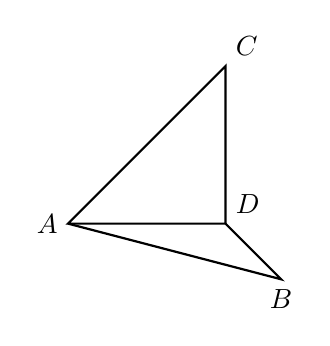
\begin{tikzpicture}[thick]
        \draw (0,0) node [left] {$A$} coordinate (A) -- (2,0) node [above right] {$D$} coordinate (D) -- (2,2) node [above right] {$C$} coordinate (C) -- cycle;
        \draw (2,0) --++ (-45:1) node [below] {$B$} coordinate (B) -- (A);
    \end{tikzpicture}
\end{center}
\item 证明: 如果共点的三条直线两两垂直, 那么它们中每两条直线所确定的平面也两两垂直.
\item 如图, $P$是平面$\alpha$外一点, 直线$PA$与平面$\alpha$斜交于点$A$, 从点$P$作平面$\alpha$上的一条直线$OA$的垂线$PO$, 垂足为$O$. 又设$a$是平面$\alpha$上的一条直线, 且$a\perp OA$, $a\perp PA$.

\begin{center}
    \begin{tikzpicture}[thick]
        \draw (-0.5,0) -- (0,0) node [above left] {$O$} -- (1,0) node [above right] {$A$} coordinate (A) -- (2,0);
        \draw (0,0) coordinate (O) -- (0,1.7) (0,1.5) node [above right] {$P$} coordinate (P);
        \draw ($(P)!{-0.1}!(A)$) -- (A);
        \draw (1.6,0) ++ (45:0.7) node [below] {$a$} --++ (225:1.4);
        \draw (0,-1.2) coordinate (X);
        \draw ($(A)!{-0.7}!(P)$) coordinate (Y);
        \draw (-0.3,0.6) -- (-1.9,-0.6) -- (2,-0.6) -- (3.2,0.6);
        \path [name path=line1] (O) -- (X);
        \path [name path=line2] (A) -- (Y);
        \path [name path=line3] (O) -- (P);
        \path [name path=line4] (A) -- (P);
        \path [name path=under_line] (-1.6,-0.6) -- (2,-0.6);
        \path [name path=above_line] (-0.3,0.6) -- (3.2,0.6);
        \path [name intersections={of = line1 and under_line, by=U}];
        \path [name intersections={of = line2 and under_line, by=V}];
        \path [name intersections={of = line3 and above_line, by=S}];
        \path [name intersections={of = line4 and above_line, by=T}];
        \draw (U) -- (X) (V) -- (Y) (-0.3,0.6) -- (S) (T) -- (3.2,0.6);
        \draw [dashed] (S) -- (T) (O) -- (X) (A) -- (Y);
    \end{tikzpicture}
\end{center}
求证: $PO\perp \text{平面}\alpha$, 从而$OA$是$PA$在平面$\alpha$上的投影.
\item 如图, 直角三角形$ABC$在平面$\alpha$上, 且$\angle BAC=90^\circ$. 以$A$为垂足作$DA\perp \alpha$, 在$DB$上取一点$E$, 使$AE\perp DB$. 求证: $CE\perp DB$.
\begin{center}
    \begin{tikzpicture}[thick]
        \draw (-1,0) -- (3,0) --++ (45:2) coordinate (R);
        \draw (-1,0) --++ (45:2) coordinate (P);
        \path [name path = aboveline] (P) -- (R);
        \draw (1,0.3) node [left] {$A$} coordinate (A) -- (2.5,0.3) node [right] {$B$} coordinate (B) -- (1,2.3) node [left] {$D$} coordinate (D);
        \draw ($(B)!{16/41}!(D)$) node [right] {$E$} coordinate (E) -- (A) -- (D);
        \path [name path = A--D] (A) -- (D);
        \path [name path = B--D] (B) -- (D);
        \path [name intersections = {of = aboveline and A--D, by = U}];
        \path [name intersections = {of = aboveline and B--D, by = V}];
        \draw [dashed] (U) -- (V);
        \draw (P) -- (U) (V) -- (R);
        \draw [dashed] (A) ++ (45:1) node [left] {$C$} coordinate (C) -- (A) (C) -- (E) (C) -- (B); 
        \draw (R) --++ (-0.3,0) node [below left] {$\alpha$};
    \end{tikzpicture}
\end{center}
\item 设平面$\alpha$与平面$\beta$平行, $A\in \alpha$, $B\in \beta$, $C$是$AB$的中点. 当$A$、$B$分别在$\alpha$、$\beta$上
运动时, 所有的动点$C$是否保持在同一个平面上? 证明你的结论.
\item 在长方体$ABCD-A_1B_1C_1D_1$中, 如果对角线$AC_1$与过点$A$的相邻三个面所成的角分别为$\alpha$、$\beta$、$\gamma$, 那么$\cos^2\alpha+\cos^2\beta+\cos^2\gamma=$\blank{50}.
\begin{center}
    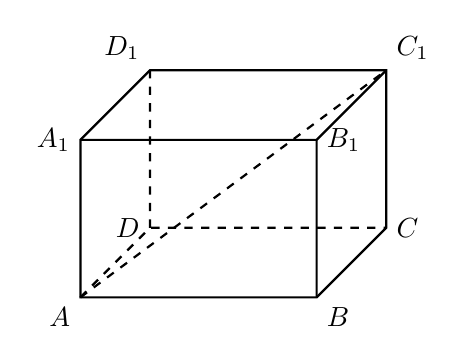
\begin{tikzpicture}[thick]
        \draw (0,0) node [below left] {$A$} coordinate (A) --++ (3,0) node [below right] {$B$} coordinate (B) --++ (45:{2.5/2}) node [right] {$C$} coordinate (C)
        --++ (0,2) node [above right] {$C_1$} coordinate (C1)
        --++ (-3,0) node [above left] {$D_1$} coordinate (D1) --++ (225:{2.5/2}) node [left] {$A_1$} coordinate (A1) -- cycle;
        \draw (A) ++ (3,2) node [right] {$B_1$} coordinate (B1) -- (B) (B1) --++ (45:{2.5/2}) (B1) --++ (-3,0);
        \draw [dashed] (A) --++ (45:{2.5/2}) node [left] {$D$} coordinate (D) --++ (3,0) (D) --++ (0,2);
        \draw [dashed] (A) -- (C1);
    \end{tikzpicture}
\end{center}
\item 如图, 该几何体是由哪个平面图形旋转得到的? 画出其余平面图形旋转得到的几何体.
\begin{center}
    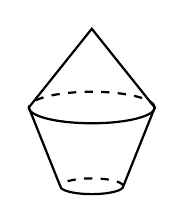
\begin{tikzpicture}[thick]
        \draw (0.4,0) -- (0.8,1) -- (0,2) -- (-0.8,1) -- (-0.4,0);
        \draw (0.4,0) arc (0:-180:0.4 and 0.1) (0.8,1) arc (0:-180:0.8 and 0.2);
        \draw [dashed] (0.4,0) arc (0:180:0.4 and 0.1) (0.8,1) arc (0:180:0.8 and 0.2);
    \end{tikzpicture}
\end{center}
\fourch{\begin{center}
    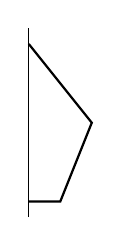
\begin{tikzpicture}[thick]
        \draw [thin] (0,-0.2) -- (0,2.2);
        \draw (0,0) -- (0.4,0) -- (0.8,1) -- (0,2);
    \end{tikzpicture}
\end{center}}{    
\begin{center}
    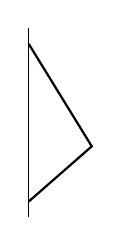
\begin{tikzpicture}[thick]
        \draw [thin] (0,-0.2) -- (0,2.2);
        \draw (0,0) -- (0.8,0.7) -- (0,2);
    \end{tikzpicture}
\end{center}}{    
\begin{center}
    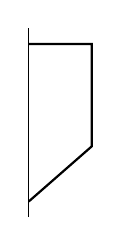
\begin{tikzpicture}[thick]
        \draw [thin] (0,-0.2) -- (0,2.2);
        \draw (0,0) -- (0.8,0.7) -- (0.8,2) -- (0,2);
    \end{tikzpicture}
\end{center}}{    
\begin{center}
    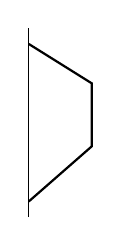
\begin{tikzpicture}[thick]
        \draw [thin] (0,-0.2) -- (0,2.2);
        \draw (0,0) -- (0.8,0.7) -- (0.8,1.5) -- (0,2);
    \end{tikzpicture}
\end{center}}
\item 判断下列命题是否正确, 并说明理由:\\
(1) 以直角三角形的一直角边为轴旋转所形成的旋转体是圆锥;\\
(2) 以直角梯形的一腰为轴旋转所形成的旋转体是圆台;\\
(3) 圆柱、圆锥、圆台都有两个底面;\\
(4) 圆锥的侧面展开图为扇形, 这个扇形所在圆的半径等于圆锥底面圆的半径.
\item 已知一个圆锥的侧面展开图恰是一个半圆. 用通过圆锥的轴的平面截此圆锥, 求截面三角形的顶角.
\item 过圆锥高的三等分点分别作平行于底面的截面, 求它们把圆锥侧面分成的三部分的面积之比.
\item 在棱长为1的正方体上, 用过同一顶点的三条棱中点的平面分别截该正方体, 截去$8$个三棱锥. 求剩下的几何体的体积.
\item 已知长方体一个顶点上的三条棱长分别是$3$、$4$、$5$, 且它的$8$个顶点都在同一球面上. 求这个球的表面积.
\item 在等边圆柱(底面直径等于高的圆柱)、球、正方体的体积相等的情况下, 讨论它们的表面积的大小关系.
\item 如图, 在三棱柱的侧棱$A_1A$和$B_1B$上分别取$P$、$Q$两点, 使$PQ$平分侧面$ABB_1A_1$的面积. 求平面$PQC$把棱柱所分成的两部分的体积之比.
\begin{center}
    \begin{tikzpicture}[thick]
        \draw (0,0) node [left] {$C$} coordinate (C) -- (3,0) node [right] {$A$} coordinate (A);
        \draw [dashed] (1,1) node [above right] {$B$} coordinate (B) -- (A) (B) -- (C) (B) --++ (0,2) node [above] {$B_1$} coordinate (B1);
        \draw (A) --++ (0,2) node [right] {$A_1$} coordinate (A1) -- (B1) -- (0,2) node [left] {$C_1$} coordinate (C1); 
        \draw (C) -- (C1) -- (A1);
        \draw ($(A)!0.7!(A1)$) node [right] {$P$} coordinate (P) -- (C);
        \draw [dashed] (P) -- ($(B)!0.3!(B1)$) node [left] {$Q$} -- (C);
    \end{tikzpicture}
\end{center}
\item 已知用通过圆锥的轴的平面去截一个圆锥, 得到的截面是面积为$9\sqrt 3\text{cm}^2$的正三角形. 求此圆锥内接球的半径.
\item 若一个长方体长、宽、高之比为$2:1:3$, 表面积为$22$, 求它的体积.
\item 如果两个球的体积之比为$8:27$, 求这两个球的表面积之比.
\item 设点$O_1$为圆锥的高靠近顶点的三等分点, 求过$O_1$与底面平行的截面面积与底面面积之比.
\item 若棱锥的高为$16$, 底面积为$256$, 平行于底面的截面面积为$50$, 求该截面与棱锥底面之间的距离.
\item 设圆锥的母线长为$1$, 高为$\dfrac{1}{2}$, 过圆锥的任意给定的两条母线作一个截面. 求截面面积的最大值.
\item 将若干毫升水倒入底面半径为$2\text{cm}$的圆柱形器皿中, 量得水面高度为$6\text{cm}$. 若将这些水倒入底面半径等于母线的倒圆锥形器皿中, 且恰好装满, 求圆锥形器皿的高.
\item 已知长方体$ABCD-A_1B_1C_1D_1$的三条棱长分别为$3\text{cm}$、$2\text{cm}$、$1\text{cm}$, 求表面有一只蜘蛛从$A$爬行到$C_1$的最短距离.
\item 如图, 已知点$P$在圆柱$O_1O$的底面圆$O$的圆周上, $AB$为圆$O$的直径, 圆柱的表面积为$20\pi$ , $OA=2$, $\angle AOP=120^\circ$.
\begin{center}
    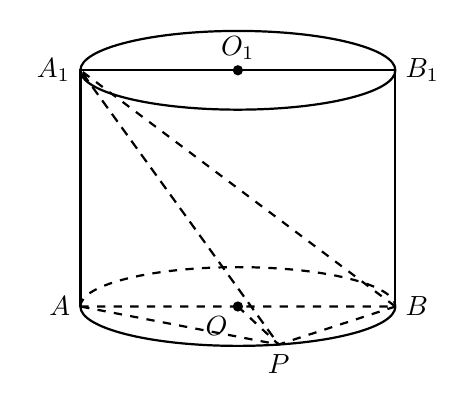
\begin{tikzpicture}[thick]
        \draw (0,0) node [left] {$A$} -- (0,3) node [left] {$A_1$} -- (4,3) node [right] {$B_1$} -- (4,0) node [right] {$B$};
        \draw (0,0) arc (180:360:2 and 0.5) (0,3) arc (180:360:2 and 0.5) (0,3) arc (180:0:2 and 0.5);
        \draw [dashed] (0,0) arc (180:0:2 and 0.5);
        \filldraw (2,0) circle (0.05) node [below left] {$O$} coordinate (O) (2,3) circle (0.05) node [above] {$O_1$} coordinate (O1);
        \draw [dashed] (0,0) -- (4,0) -- (0,3) -- ({2+2*cos(-75)},{0.5*sin(-75)}) node [below] {$P$} coordinate (P) (O) -- (P) -- (0,3) (4,0) -- (P) -- (0,0);
    \end{tikzpicture}
\end{center}
(1) 求三棱锥$A_1-ABP$的体积;\\
(2) 求异面直线$A_1B$与$AP$所成角的大小.
\item 如图, 在圆柱中, 底面直径$AB$等于母线$AD$, 点$E$在底面的圆周上, 且$AF\perp DE$, $F$是垂足.
\begin{center}
    \begin{tikzpicture}[thick]
        \draw (0,0) node [left] {$A$} -- (0,3) node [left] {$D$} coordinate (D) (3,3) node [right] {$C$} -- (3,0) node [right] {$B$};
        \draw (0,0) arc (180:360:1.5 and 0.5) (0,3) arc (180:-180:1.5 and 0.5);
        \draw [dashed] (0,0) arc (180:0:1.5 and 0.5);
        \draw [dashed] ({1.5+1.5*cos(-105)},{0.5*sin(-105)}) node [below] {$E$} coordinate (E) -- (0,0) (E) -- (3,0) (E) -- (0,3) -- (3,0) -- (0,0) -- ($(E)!0.3!(D)$) node [left] {$F$};
    \end{tikzpicture}
\end{center}
(1) 求证: $AF\perp DB$;\\
(2) 若圆柱与三棱锥$D-ABE$的体积的比等于$3\pi$ , 求直线$DE$与平面$ABD$所成角的大小.
\item 如图, 半球内有一内接正方体(即正方体的一个面在半球的底面圆上, 其余顶点在半球面上). 若正方体的棱长为$\sqrt 6$, 求半球的表面积和体积. 
\begin{center}
    \begin{tikzpicture}[thick]
        \draw [dashed] (0,0)  coordinate (A) --++ (2,0)  coordinate (B) --++ (45:{2/2})  coordinate (C)
        --++ (0,2)  coordinate (C1) --++ (-2,0)  coordinate (D1) --++ (225:{2/2}) coordinate (A1) -- cycle;
        \draw [dashed] (A) ++ (2,2) coordinate (B1) -- (B) (B1) --++ (45:{2/2}) (B1) --++ (-2,0);
        \draw [dashed] (A) --++ (45:{2/2})  coordinate (D) --++ (2,0) (D) --++ (0,2);        
        \draw ($(A)!0.5!(C)$) ++ ({-sqrt(6)},0) coordinate (L)  arc (180:0:{sqrt(6)});
        \draw (L) arc (-180:0:{sqrt(6)} and {sqrt(6)/3});
        \draw [dashed] (L) arc (180:0:{sqrt(6)} and {sqrt(6)/3});
    \end{tikzpicture}
\end{center}
\item 已知圆锥的底面半径为$r$, 高为$h$, 正方体$ABCD-A_1B_1C_1D_1$内接于该圆锥. 求这个正方体的棱长.
\item 如图, 一个圆锥形的空杯子上放着一个半球形的冰激凌, 如果冰激凌融化了, 会溢出来吗?
\begin{center}
    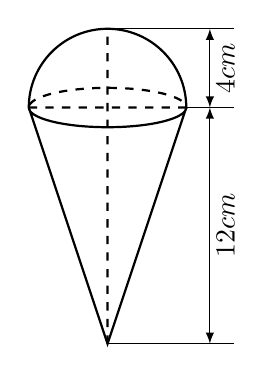
\begin{tikzpicture}[thick,>=latex]
        \draw (-1,0) -- (0,-3) -- (1,0) arc (0:180:1) arc (180:360:1 and 0.25);
        \draw [dashed] (0,-3) -- (0,1) (-1,0) -- (1,0) arc (0:180:1 and 0.25);
        \draw [thin] (1,0) -- (1.6,0) (0,-3) -- (1.6,-3) (0,1) -- (1.6,1);
        \draw [thin,<->] (1.3,0) -- (1.3,1);
        \draw [thin,<->] (1.3,0) -- (1.3,-3);
        \draw (1.5,0.5) node {\rotatebox{90}{$4\text{cm}$}};
        \draw (1.5,-1.5) node {\rotatebox{90}{$12\text{cm}$}};
    \end{tikzpicture}
\end{center}
\item 如图, 用一块钢锭浇铸一个厚度均匀, 且表面积为$2\text{m}^2$的正四棱锥形有盖容器. 设容器的高为$h\text{m}$, 盖子的边长为$a\text{m}$.
\begin{center}
    \begin{tikzpicture}[thick]
        \draw (0,0) node [above] {$A$} -- (3,0) node [right] {$B$} coordinate (B) --++ (135:1.5) node [above] {$C$} coordinate (C) --++ (-3,0) node [above] {$D$} coordinate (D) -- cycle;
        \draw ($(B)!0.5!(D)$) ++ (0,-2) node [below] {$P$} coordinate (P) (P) -- (0,0) (P) -- (D) (P) -- (B);
        \draw [dashed] (P) -- (C);
    \end{tikzpicture}
\end{center}
(1) 求$a$关于$h$的函数表达式;\\
(2) 当$h$为何值时, 容器的容积$V$最大? 并求出$V$的最大值.
\item 将一块边长为$10\text{cm}$的正方形铁片裁下如图所示的阴影部分, 用余下的四个全等的等腰三角形加工成一个无盖的正四棱锥形容器罩.
\begin{center}
    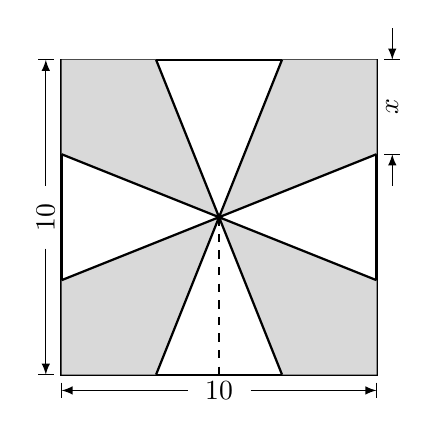
\begin{tikzpicture}[thick,>=latex]
        \draw (-2,-2) -- (-2,2) -- (2,2) -- (2,-2) -- cycle;
        \fill [gray!30] (0,0) -- (0.8,2) -- (2,2) -- (2,0.8) -- cycle;
        \fill [gray!30] (0,0) -- (-0.8,2) -- (-2,2) -- (-2,0.8) -- cycle;
        \fill [gray!30] (0,0) -- (0.8,-2) -- (2,-2) -- (2,-0.8) -- cycle;
        \fill [gray!30] (0,0) -- (-0.8,-2) -- (-2,-2) -- (-2,-0.8) -- cycle;
        \draw (0.8,-2) -- (-0.8,2) (-0.8,-2) -- (0.8,2) (-2,0.8) -- (2,-0.8) (-2,-0.8) -- (2,0.8);
        \draw [dashed] (0,0) -- (0,-2);
        \draw [thin] (-2,-2.1) -- (-2,-2.3) (2,-2.1) -- (2,-2.3) (-2.1,-2) -- (-2.3,-2) (-2.1,2) -- (-2.3,2) (2.1,2) -- (2.3,2) (2.1,0.8) -- (2.3,0.8);
        \draw [->,thin] (-0.4,-2.2) -- (-2,-2.2);
        \draw [->,thin] (0.4,-2.2) -- (2,-2.2);
        \draw [->,thin] (-2.2,-0.4) -- (-2.2,-2);
        \draw [->,thin] (-2.2,0.4) -- (-2.2,2);
        \draw [->,thin] (2.2,0.4) -- (2.2,0.8);
        \draw [->,thin] (2.2,2.4) -- (2.2,2);
        \draw (0,-2.2) node {$10$} (-2.2,0) node {\rotatebox{90}{$10$}} (2.2,1.4) node {\rotatebox{90}{$x$}};
    \end{tikzpicture}
    \begin{tikzpicture}[thick]
        \draw (0,0) node [left] {$A$} -- (3,0) node [right] {$B$} coordinate (B) --++ (45:1.5) node [right] {$C$} coordinate (C) ++ (-3,0) node [below right] {$D$} coordinate (D);
        \draw ($(B)!0.5!(D)$) node [below left] {$O$} coordinate (O) ++ (0,2) node [above] {$E$} coordinate (E) (E) -- (0,0) (E) -- (C) (E) -- (B);
        \draw [dashed] (E) -- (D);
        \draw [dashed] ($(B)!0.5!(C)$) node [right] {$F$} coordinate (F) -- (O) -- (E) (C) -- (D) -- (A);
        \draw (E) -- (F);
    \end{tikzpicture}
\end{center}
(1) 试把容器罩的表面积$S$表示为$x$的函数;\\
(2) 试把容器罩的体积$V$表示为$x$的函数.
\item 从字母$a$、$b$、$c$、$d$、$e$中任取两个, 求取到字母$a$的概率.
\item 现有$5$根细木棍, 长度(单位: $\text{cm}$)分别为$1$、$3$、$5$、$7$、$9$, 从中任取$3$根. 求能搭成一个三角形的概率.
\item 将$2$本不同的英语书和$1$本语文书在书架上随机排成一行, 求$2$本英语书相邻的概率.
\item 从编号分别为$1$、$2$、$3$、$4$、$5$、$6$的$6$个大小与质地相同的小球中随机取出$3$个, 求恰有$2$个小球编号相邻的概率.
\item 袋中装有大小与质地相同的$5$个球, 其中红色球$3$个, 标号分别为$1$、$2$、$3$; 蓝色球$2$个, 标号分别为$1$、$2$. 从袋中任取$2$个球, 求这$2$个球颜色不同且标号之和不小于$4$的概率.
\item 袋中装有大小与质地相同的$5$个球, 其中白球$3$个, 黑球$2$个, 从中一次摸出$2$个球.\\
(1) 写出该随机试验的一个等可能的样本空间;\\
(2) 求摸出来的$2$个球都是白球的概率;\\
(3) 求摸出来的$2$个球颜色不同的概率.
\item 对某工厂生产的产品质量进行抽查, 数据如下表所示.
\begin{center}
    \begin{tabular}{|c|c|c|c|c|c|}
        \hline
        抽查件数 & $50$ & $100$ & $200$ & $300$ & $500$\\ \hline
        合格件数 & $47$ & $95$ & $192$ & $285$ & $478$\\ \hline        
    \end{tabular}
\end{center}
根据上表所提供的数据, 问: 合格品的概率约为多少?(结果保留两位小数)
\item 射击队某选手命中环数的概率如下表所示.
\begin{center}
    \begin{tabular}{|c|c|c|c|c|}
        \hline
        命中环数 & $10$ & $9$ & $8$ & $7$\\ \hline
        概率 & $0.32$ & $0.28$ & $0.18$ & $0.12$ \\ \hline        
    \end{tabular}
\end{center}
该选手射击一次, 求:\\
(1) 命中$9$环或$10$环的概率;\\
(2) 至少命中$8$环的概率;\\
(3) 命中不足$8$环的概率.
\item 某学生做两道选择题, 已知每道题均有$4$个选项, 其中有且只有一个正确答案. 该学生随意填写两个答案, 求两个答案都选错的概率.
\item 盒子中有标号为$1$、$2$、$3$的$3$个大小与质地相同的球, 随机地取$1$个球, 放回后再取$1$个球, 把这$2$个球对应的号码按照取的先后顺序组成一个两位数. 求个位数与十位数不相同的概率.
\item 一个盒子中装有$4$张卡片, 卡片上分别写有数字$1$、$2$、$3$、$4$. 现从盒子中随机抽取卡片.\\
(1) 若一次抽取$3$张卡片, 求$3$张卡片上数字之和大于$7$的概率;\\
(2) 若第一次抽取$1$张卡片, 放回后再抽取$1$张卡片, 求两次抽取的卡片上数字之和大于$7$的概率.
\item 盒子中有散落的黑白棋子若干粒, 已知从中取出$2$粒都是黑子的概率是$\dfrac 17$, 从中取出$2$粒都是白子的概率是$\dfrac 16$. 问: 从中任意取出$2$粒恰好是同一颜色的概率是多少?
\item 社会调查人员总希望从对人群的随机抽样调查中得到对他们所提问题的诚实回答, 但是被采访者常常不愿意如实做出应答. 1965年, 华纳(Stanley L. Warner)发明了一种应
用概率知识来消除这种不愿意如实回答的情绪的方法. 华纳的随机化应答方法要求人们随机地回答所提两个问题中的一个, 而不必告诉采访者究竟回答的是哪个问题, 在这两个问题中有一个是敏感的或者令人为难的, 另一个则是无关紧要的. 这样, 应答者将乐意如实地回答问题, 因为只有他自己知道回答的是哪个问题. 例如, 在调查运动员是否服用兴奋剂的时候, 设计一个从袋中摸球的试验: 袋中放有$1$黑$1$白两个大小与质地相同的小球, 运动员从中随意摸出$1$个小球. 无关紧要的问题是: 你摸出的小球是白色的吗? 而敏感的问题是: 你服用过兴奋剂吗? 然后要求被调查的运动员抛掷一枚硬币, 如果出现正面, 就回答第一个问题, 否则回答第二个问题. 假设用这个方法调查了$200$名运动员, 得到$56$个``是''的回答, 请你估计这群运动员中大约有百分之几的人服用过兴奋剂.
\item 在一次知识竞赛中, 假设$A$、$B$、$C$、$D$四人独立答题, 且答对的概率分别为$P(A)=\dfrac 13$, $P(B)=\dfrac 14$, $P(C)=\dfrac 15$, $P(D)=\dfrac 23$, 如果将$A$、$B$、$C$组成一组与$D$比赛, 且$A$、$B$、$C$三人中有一人答对即算该组答对, 那么哪一方答对的概率大?
\item 某高校研究人员希望调查该校大学生平均每天的自习时间. 他调查了$100$名大学生, 发现他们每天的平均自习时间是$3.5\text{h}$. 这里的总体是\bracket{20}.
\onech{该校的所有大学生}{该校所有大学生的平均每天自习时间}{所调查的$100$名大学生}{所调查的$100$名大学生的平均每天自习时间}
\item 某家大型超市的日客流量(单位: 千人次)分别为: $3.4$、$3.6$、$5.6$、$1.8$、$3.7$、$4.0$、$2.5$、$2.8$、$4.4$、$3.6$. 下列图形中不利于描述这些数据的是\bracket{20}.
\fourch{散点图}{条形图}{茎叶图}{扇形图}
\item 某汽车销售商销售某品牌的A、B、C三类轿车, 每类轿车均有舒适型和经济型两种型号, 其某月的销量(单位: 辆)如下表所示.
\begin{center}
    \begin{tabular}{|c|c|c|c|}
        \hline
        & A & B & C \\ \hline
        舒适型/辆 & $35$ & $28$ & $15$\\ \hline
        经济型/辆 & $50$ & $72$ & $40$\\ \hline
    \end{tabular}
\end{center}
试设计一个抽样方案, 从该月购买轿车的客户中抽取20位, 调查他们的满意度.
\item 某校$30$名高一女生的扔手球记录如下(单位: $\text{m}$):
\begin{center}
    \begin{tabular}{cccccccccc}
        $16.3$ & $13.2$ & $17.7$ & $14.3$ & $16.4$ & $19.8$ & $13.5$ & $14.5$ & $11.7$ & $14.1$\\
        $14.8$ & $17.2$ & $13.8$ & $15.4$ & $16.3$ & $15.7$ & $18.5$ & $16.8$ & $17.9$ & $15.9$\\
        $17.6$ & $15.4$ & $16.8$ & $21.4$ & $16.5$ & $18.1$ & $16.0$ & $20.3$ & $16.6$ & $19.5$
    \end{tabular}
\end{center}
(1) 选择适当的组距, 制作一张频率分布表;\\
(2) 在(1)的基础上, 绘制一幅频率分布直方图.
\item 某公司对应聘人员进行能力测试, 测试成绩总分为150分, 下面是50位应聘人员
的测试成绩:
\begin{center}
    \begin{tabular}{cccccccccc}
        $64$ & $67$ & $70$ & $72$ & $74$ & $76$ & $76$ & $79$ & $80$ & $81$ \\
        $82$ & $82$ & $83$ & $85$ & $86$ & $88$ & $91$ & $91$ & $92$ & $93$ \\
        $93$ & $93$ & $95$ & $96$ & $96$ & $97$ & $97$ & $99$ & $100$ & $100$ \\
        $102$ & $104$ & $106$ & $106$ & $107$ & $108$ & $108$ & $112$ & $112$ & $114$ \\
        $116$ & $118$ & $119$ & $119$ & $122$ & $123$ & $125$ & $126$ & $128$ & $133$
    \end{tabular}
\end{center}
试用这些数据绘制一幅茎叶图.
\item 某超市从一家食品有限公司购进一批茶叶, 每罐茶叶的标准质量是$125\text{g}$, 为了解该批茶叶的质量情况, 从中随机抽取$20$罐, 称得各罐质量(单位: $\text{g}$)如下:
\begin{center}
    \begin{tabular}{ccccccc}
        $124.9$ & $124.7$ & $126.2$ & $124.9$ & $124.2$ & $124.9$ & $123.7$ \\
        $121.4$ & $126.4$ & $127.7$ & $121.9$ & $124.4$ & $125.2$ & $123.7$ \\
        $122.7$ & $124.2$ & $126.2$ & $125.2$ & $122.2$ & $125.4$
    \end{tabular}
\end{center}
回答下列问题:\\
(1) $20$罐茶叶的平均质量$\bar{x}$是多少, 标准差$s$是多少?
(2) 有多少罐茶叶的质量位于$\bar x-s$与$\bar x +s$之间, 所占的百分比是多少?
\item 数据$x_1$、$x_2$、$\cdots$、$x_n$的方差为$s_x^2$, 数据$y_1$、$y_2$、$\cdots$、$y_n$的方差为$s_y^2$, 若$y_1=ax_1+b$, $y_2=ax_2+b$, $\cdots$, $y_n=ax_n+b$成立, $a$、$b$为常数, 求证: $s_y^2=a^2s_x^2$.
\item 下表是上海市$2007$年至$2016$年的月平均气温(单位: $^\circ\text{C}$).
\begin{center}
    \begin{tabular}{|c|c|c|c|c|c|c|c|c|c|c|c|c|}
        \hline
        年份 & $1$月 & $2$月 & $3$月 & $4$月 & $5$月 & $6$月 & $7$月 & $8$月 & $9$月 & $10$月 & $11$月 & $12$月 \\ \hline
        $2007$ & $5.9$ & $9.8$ & $12.1$ & $15.9$ & $22.9$ & $25$ & $30.4$ & $29.7$ & $25.4$ & $20.6$ & $14.2$ & $9.8$ \\ \hline
        $2008$ & $4.5$ & $4.2$ & $11.6$ & $16.1$ & $21.8$ & $24.2$ & $30.4$ & $28.6$ & $26$ & $21$ & $13.3$ & $7.9$ \\ \hline
        $2009$ & $4.3$ & $9.3$ & $10.8$ & $16.7$ & $22.5$ & $26.3$ & $29$ & $28.1$ & $25.4$ & $21.4$ & $12.4$ & $6.9$ \\ \hline
        $2010$ & $5.7$ & $7.7$ & $9.6$ & $13.3$ & $20.9$ & $24.1$ & $28.8$ & $30.9$ & $26.2$ & $19.3$ & $14.2$ & $8.1$\\ \hline
        $2011$ & $1.9$ & $6.5$ & $9.5$ & $16.2$ & $21.9$ & $24.4$ & $30.2$ & $28.3$ & $24.7$ & $19.3$ & $16.7$ & $6.9$\\ \hline
        $2012$ & $5.1$ & $4.8$ & $9.8$ & $17.6$ & $21.6$ & $24.7$ & $29.9$ & $29$ & $23.9$ & $20.1$ & $12.6$ & $6.6$\\ \hline
        $2013$ & $4.6$ & $6.8$ & $11$ & $15.3$ & $21.3$ & $24.1$ & $32$ &  $31$ & $25$ & $20$ & $13.4$ & $6.1$\\ \hline
        $2014$ & $6.6$ & $6.1$ & $11.5$ & $15.7$ & $21.7$ & $23.3$ & $27.4$ & $26.3$ & $24.2$ & $20.2$ & $14.8$ & $5.7$\\ \hline
        $2015$ & $6$ & $6.8$ & $10.6$ & $15.9$ & $20.5$ & $24.2$ & $26.7$ & $27.8$ & $24.2$ & $19.6$ & $14$ & $7.8$\\ \hline
        $2016$ & $4.4$ & $6.9$ & $11$ & $16.7$ & $20.6$ & $24.2$ & $29.9$ & $29.5$ & $24.9$ & $20.8$ & $13.6$ & $9.1$\\ \hline
    \end{tabular}
\end{center}
\begin{flushright}
{\it 数据来源: 上海统计年鉴.}
\end{flushright}
回答下列问题:\\
(1) $10$年中每年最冷的月份相同吗?\\
(2) $10$年中哪个月份的气温波动最大?\\
(3) $10$年中哪一年的气温波动最大?\\
(4) 绘制$10$年中$7$月份与$8$月份气温的折线图, 比较气温的高低.
\item 某高校数学专业共有$850$名学生, 从中选取$20$名学生参加学生代表大会. 试写出具体抽样方案.
\item 某校高一年级学生进行了$4$次测验, 成绩(单位: 分)如下表所示. 根据$4$次测验的结果, 我们如何比较这$10$名学生的成绩? 下周有一场数学竞赛活动, 如果需要$1$名学生参赛, 那么推荐谁去最好? 如果需要$4$名学生参赛, 那么又该推荐谁去?
\begin{center}
    \begin{tabular}{|c|c|c|c|c|}
        \hline
        学生编号 & 第$1$次 & 第$2$次 & 第$3$次 & 第$4$次 \\ \hline
        $1$ & $90$ & $82$ & $97$ & $100$ \\ \hline
        $2$ & $103$ & $86$ & $101$ & $92$ \\ \hline
        $3$ & $77$ & $83$ & $106$ & $87$ \\ \hline
        $4$ & $94$ & $93$ & $99$ & $99$ \\ \hline 
        $5$ & $89$ & $97$ & $93$ & $90$\\ \hline
        $6$ & $101$ & $79$ & $87$ & $95$\\ \hline
        $7$ & $91$ & $92$ & $91$ & $93$ \\ \hline
        $8$ & $82$ & $94$ & $100$ & $106$ \\ \hline
        $9$ & $88$ & $78$ & $95$ & $78$ \\ \hline
        $10$ & $83$ & $88$ & $104$ & $89$ \\ \hline        
    \end{tabular}
\end{center}
\item 某客服部门计划根据员工每个月接通的电话数给予奖金奖励, 并且要保证$50\%$的员工能拿到基本奖励, 拿到基本奖励的员工中至多$10\%$的人能够拿到额外奖励. 该部门随
机抽取了$30$名员工, 调查了他们上半个月与客户的通话数量, 数据如下:
\begin{center}
    \begin{tabular}{cccccccccc}
        $1344$ & $1428$ & $1083$ & $1239$ & $1381$ & $1099$ & $1607$ & $1041$ & $1130$ & $1610$ \\
        $1445$ & $921$ & $931$ & $1100$ & $1197$ & $1282$ & $1549$ & $1463$ & $901$ & $1354$ \\
        $1378$ & $1752$ & $1032$ & $968$ & $902$ & $1804$ & $1051$ & $1319$ & $1223$ & $1124$
    \end{tabular}
\end{center}
请利用百分位数来为该部门设计奖励方案.
\item 求直线$\sqrt 2x-4y+5=0$的倾斜角(用$\arctan$表示).
\item 若直线$ax+2y+6=0$和直线$x+a(a+1)y+(a^2-1)=0$互相垂直, 求实数$a$的值.
\item 直线$x-y+1=0$上一点$P$的横坐标是$3$, 若该直线绕点$P$逆时针旋转$90^\circ$得到直线$l$, 求直线$l$的方程.
\item 设直线$x-ay-4=0$与直线$y=-2x+4$的夹角为$\arccos \dfrac{2\sqrt 5}5$, 求实数$a$的值.
\item 已知$\alpha\in [0, \dfrac\pi 2)$, 求直线$x\cos \alpha+\sqrt 3y+2=0$的倾斜角的取值范围.
\item 求过点$(3, -2)$且在$x$轴、$y$轴上截距相等的直线的方程.
\item 已知点$P(1, 1)$到直线$x+ay-2=0$的距离为$1$, 求实数$a$的值.
\item 已知平行四边形$ABCD$中, 边$AB$所在直线的方程为$x+y-1=0$, 边$AD$所在直线的方程为$3x-y+4=0$.\\
(1) 求点$A$的坐标;\\
(2) 若点$C$的坐标为$(3, 3)$, 分别求边$BC$与$DC$所在直线的方程.
\item 已知直线$l_1: x+my+6=0$, $l_2: (m-2)x+3y+2m=0$, 求实数$m$的取值范围, 使得:\\
(1) $l_1$与$l_2$相交;\\
(2) $l_1\perp l_2$;\\
(3) $l_1\parallel l_2$;\\
(4) $l_1$与$l_2$重合.
\item 已知直线$l$与两坐标轴围成一个等腰直角三角形, 且此三角形的面积为$\dfrac{49}2$. 求直线$l$的方程.
\item 在$\triangle ABC$中, 边$AB$、$AC$上的高所在直线的方程分别为$2x-3y+1=0$与$x+y=0$, 点$A$的坐标为$(1, 2)$. 求边$BC$所在直线的方程.
\item 已知直线$l$垂直于直线$3x+4y-9=0$, 点$A(2, 3)$到直线$l$的距离为$1$. 求直线$l$的方程.
\item 已知三条直线$l_1: ax+by+4=0$, $l_2: (a-1)x+y+b=0$, $l_3: x+2y+3=0$.\\
(1) 若$l_1\perp l_2$且$l_1$经过点$(-1, 1)$, 求$a$、$b$的值;\\
(2) 若$l_1\parallel l_2\parallel l_3$, 求$a$、$b$的值.
\item 已知过点$(0, -2)$且具有斜率$k$的直线$l$与以点$A(3, 1)$和$B(-2, 5)$为端点的线段$AB$相交, 求实数$k$的取值范围.
\item 已知两条直线$l_1: y-x=0$, $l_2: y=ax$, 其中$a\in \mathbf{R}$. 当这两条直线的夹角在$(0, \dfrac{\pi}{12})$内变化时, 求实数$a$的取值范围.
\item 直线$l$过原点且平分平行四边形$ABCD$的面积, 若此平行四边形的两个顶点为$B(1, 4)$、$D(5, 0)$, 求直线$l$的方程.
\item 求直线$l_1: 3x-2y-6=0$关于直线$l_2: 2x-3y+1=0$对称的直线$l_3$的方程.
\item 已知动点$M(a, b)$在直线$3x+4y-15=0$上, 求$\sqrt{a^2+b^2}$的最小值.
\item 已知两条平行直线$l_1$与$l_2$分别过点$P_1(1, 0)$与点$P_2(0, 5)$, $l_1$、$l_2$之间的距离为$d$. 求$d$的最大值, 并指出此时$l_1$、$l_2$的方程.
\item 已知直线$l$经过点$C(2, 1)$, 且与$x$轴、$y$轴的正半轴分别交于点$A$、点$B$, $O$是坐标原点.\\
(1) 当$\triangle AOB$的面积最小时, 求直线$l$的方程;\\
(2) 当$|CA|\cdot |CB|$取最小值时, 求直线$l$的方程, 并求此最小值.
\item 作出方程$|x|+|y|=1$所表示的图形, 并求该图形围成的区域的面积.
\item 给定直线$l_1: y=k_1x+b_1$与$l_2: y=k_2x+b_2$, 求证: 如果直线$l_1$与$l_2$不互相垂直, 那么它们的夹角$\alpha$满足$\tan \alpha=|\dfrac{k_1-k_2}{1+k_1k_2}|$.
\item 已知直线$l_1: 4x+y=4$, $l_2: mx+y=0$, $l_3: 2x-3my=4$. 当$m$为何值时, 它们不能围成三角形?
\item 点到直线的距离是该点到直线上任意一点距离的最小值. 如果把一个给定点到线段上任意一点的距离的最小值定义为该点到该线段的距离, 试求点$P(1, 1)$到线段$l: x-
y-3=0 \ (3\le x\le 5)$的距离.
\item 判断下列命题是否正确, 并说明理由:\\
(1) 到两坐标轴距离相等的点的轨迹方程为$y=x$;\\
(2) 若$\triangle ABC$的三个顶点的坐标分别为$A(1, 1)$、$B(3, 1)$、$C(1, 3)$, 则边$BC$上的中线所在直线的方程为$y=x$;\\
(3) 与两点$A(-1, 0)$、$B(1, 0)$的连线的夹角为$90^\circ$的动点的轨迹方程为$x^2+y^2=1$.
\item 讨论圆$x^2+y^2+6x-7=0$与抛物线$y^2=-4x$准线的位置关系.
\item 对圆$(x-a)^2+(y+b)^2=a^2+b^2\ (a>0, \ b>0)$, 下列说法是否正确, 请说明理由:\\
(1) 该圆的圆心为$(a, b)$;\\
(2) 该圆过原点;\\
(3) 该圆与$x$轴相交于两个不同点.
\item 若椭圆$\dfrac{x^2}{4}+\dfrac{y^2}{a^2}=1$与双曲线$\dfrac{x^2}{a^2}-\dfrac{y^2}2=1$有相同的焦点, 求实数$a$的值.
\item 设椭圆$\dfrac{x^2}{a^2}+\dfrac{y^2}{b^2}=1 \ (a>b>0)$的焦距为$2c$. 若$b^2=ac$, 求该椭圆的离心率.
\item 已知圆$C$的半径为$3$, 它与双曲线$\dfrac{x^2}4-y^2=1$的两条渐近线均相切, 且与该双曲线的右支相交. 求圆$C$的方程.
\item 已知直线$y=x+b$被曲线$y=\dfrac 12x^2$截得的弦长为$4\sqrt 2$, 求实数$b$的值.
\item 点$P$是圆$x^2+y^2=4$上的动点, 过点$P$作$x$轴的垂线, 垂足为$M$. 若$\overrightarrow{PQ}=2\overrightarrow{QM}$, 求点$Q$的轨迹方程.
\item 设$AB$是过抛物线$y^2=2px$焦点$F$的一条弦, 过点$A$、$B$分别作该抛物线准线的垂线, 垂足分别为$A_1$、$B_1$. 求证: $\angle A_1FB_1=\dfrac\pi 2$.
\item 已知圆$O$的方程是$x^2+y^2=1$, 直线$l$与圆$O$相切.\\
(1) 若直线$l$的斜率等于$1$, 求直线$l$的方程;\\
(2) 若直线$l$在$y$轴上的截距为$\sqrt 2$, 求直线$l$的方程.
\item 直线$x-\sqrt 3y=0$绕原点按逆时针方向旋转$30^\circ$后所得的直线$l$与圆$(x-2)^2+y^2=3$的位置关系是\bracket{20}.
\twoch{直线$l$过圆心}{直线$l$与圆相交, 但不过圆心}{直线$l$与圆相切}{直线$l$与圆无公共点}
\item 已知点$A(-\dfrac 12, 0)$, $B$是圆$C: (x-\dfrac 12)^2+y^2=4$($C$是圆心)上一动点, 线段$AB$的垂直平分线交$BC$于$M$. 求动点$M$的轨迹方程.
\item 过抛物线$y^2=4x$的焦点$F$作动直线交抛物线于$A$、$B$两点, 并从原点$O$作$AB$的垂线, 垂足为$M$. 求动点$M$的轨迹方程.
\item 已知点$P$是双曲线$\dfrac{x^2}9-\dfrac{y^2}{16}=1$右支上的一点, 点$M$、$N$分别是圆$(x+5)^2+y^2=4$和$(x-5)^2+y^2=1$上的点. 求$|PM|-|PN|$的最大值.
\item 已知圆$x^2+y^2+x-6y+m=0$与直线$x+2y-3=0$相交于$P$、$Q$两点, $O$为坐标原点. 若$OP\perp OQ$, 求实数$m$的值.
\item 已知直线$y=ax-1$与曲线$y^2=2x$只有一个公共点, 求实数$a$的值.
\item 对于实数$k$的不同取值范围, 讨论方程$kx^2+y^2-2=0$所表示的曲线的形状.
\item 过椭圆$b^2x^2+a^2y^2=a^2b^2 \ (a>b>0)$的顶点$B(0, -b)$引一条弦$BP$, 求弦$BP$的最大长度.
\item 已知定点$A(a, 0) \ (0<a<3)$到椭圆$\dfrac{x^2}9+\dfrac{y^2}4=1$上的点的距离的最小值为$1$, 求$a$的值.
\item 据气象预报, 在气象台$A$处向东$400\text{km}B$处的海面上有一个台风中心形成, 测得台风以$40\text{km}/\text{h}$的速度向西北方向移动, 距中心不超过$300\text{km}$的地方都会受到台风的影响. 从现在起, 多少时间后气象台受到台风影响?  气象台受到台风影响的时长大约是多少(结果精确到$0.1\text{h}$)?
\item 已知$\triangle ABC$的两个顶点$A$、$B$的坐标分别是$(-6, 0)$、$(6, 0)$, 且边$AC$、$BC$所在直线的斜率之积等于$k$. 讨论顶点$C$的轨迹方程.
\item 以$P$为圆心的动圆与圆$C_1: (x+2)^2+y^2=1$和圆$C_2: (x-2)^2+y^2=r^2$均相切, 请分别写出$r$的某个值, 使点$P$的轨迹为椭圆和双曲线.
\item 求双曲线$y=\dfrac 1x$的焦点坐标与准线方程.
\item 请验证到点$(1, \dfrac 14)$的距离和到直线$y=-\dfrac 14$的距离相等的动点的轨迹方程是二次函数$y=x^2-2x+1$, 并探究一般情况.
\item 求连接点$A(x, y, z)$与点$B(x', y', z')$的线段$AB$的中点$M$的坐标.
\item 设正四面体$ABCD$的棱长为$a$, $E$为$BC$的中点, $F$为$CD$的中点. 求$\overrightarrow{BF}\cdot\overrightarrow{AE}$.
\item 给定点$A(1, 0, 0)$、$B(3, 1, 1)$、$C(2, 0, 1)$与点$D(5, -4, 3)$.\\
(1) 求$\overrightarrow{AD}$在$\overrightarrow{AB}$、$\overrightarrow{BC}$、$\overrightarrow{CA}$方向上的投影向量;\\
(2) 求点$D$到平面$ABC$的距离.
\item 如图, 在正三棱柱$ABC-A_1B_1C_1$中, $|AB|=\sqrt 2|AA_1|$, $D$是$A_1B_1$的中点, 点$E$在$A_1C_1$上, 且$DE\perp AE$.
\begin{center}
    \begin{tikzpicture}[thick]
        \draw (0,0) node [left] {$A$} coordinate (A) -- (0,2) node [left] {$A_1$} coordinate (A1) --++ ({2*sqrt(2)},0) node [right] {$C_1$} coordinate (C1) --++ (0,-2) node [right] {$C$} coordinate (C);
        \draw ({sqrt(2)},0) ++ (-45:{sqrt(6)/2}) node [below] {$B$} coordinate (B) --++ (0,2) node [left] {$B_1$} coordinate (B1) (B) -- (A) (B) -- (C) (B1) -- (A1) (B1) -- (C1);
        \draw ($(A1)!0.5!(B1)$) node [above] {$D$} coordinate (D) -- ($(A1)!0.25!(C1)$) node [above] {$E$} coordinate (E);
        \draw [dashed] (E) -- (A) -- (D) (A) -- (C1) (A) -- (C);
    \end{tikzpicture}
\end{center}
(1) 求证: $\text{平面}ADE\perp \text{平面}ACC_1A_1$;\\
(2) 求直线$AD$和平面$ABC_1$所成角的大小.
\item 已知正四棱锥的体积为$12$, 底面对角线的长为$2\sqrt 6$. 求侧面与底面所成二面角的大小.
\item 如图, 已知$ABCD-A_1B_1C_1D_1$是底面边长为$1$的正四棱柱, $O_1$是$A_1C_1$和$B_1D_1$的交点.
\begin{center}
    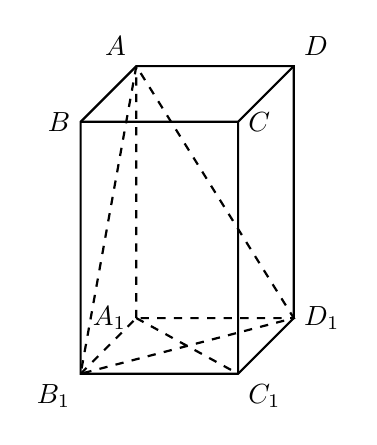
\begin{tikzpicture}[thick,scale = 2]
        \draw (0,0) node [below left] {$B_1$} coordinate (B1) --++ (1,0) node [below right] {$C_1$} coordinate (C1) --++ (45:{1/2}) node [right] {$D_1$} coordinate (D1)
        --++ (0,1.6) node [above right] {$D$} coordinate (D)
        --++ (-1,0) node [above left] {$A$} coordinate (A) --++ (225:{1/2}) node [left] {$B$} coordinate (B) -- cycle;
        \draw (B1) ++ (1,1.6) node [right] {$C$} coordinate (C) -- (C1) (C) --++ (45:{1/2}) (D) (C) --++ (-1,0);
        \draw [dashed] (B1) --++ (45:{1/2}) node [left] {$A_1$} coordinate (A1) --++ (1,0) (A1) --++ (0,1.6);
        \draw [dashed] (A) -- (B1) -- (D1) -- cycle (A1) -- (C1);
    \end{tikzpicture}
\end{center}
(1) 设$AB_1$与底面$A_1B_1C_1D_1$所成角的大小为$\alpha$, 二面角$A-B_1D_1-A_1$的大小为$\beta$. 求证: $\tan \beta=\sqrt 2\tan \alpha$;\\
(2) 若点$C$到平面$AB_1D_1$的距离为$\dfrac 43$, 求此正四棱柱的高.
\item 如图, 在直三棱柱$ABC-A_1B_1C_1$中, $\angle ACB=90^\circ$, $|AC|=|BC|=|CC_1|=2$.
\begin{center}
    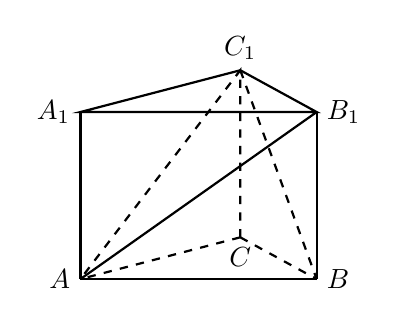
\begin{tikzpicture}[thick,scale = 1.5]
        \draw (0,0) node [left] {$A$} coordinate (A) -- (2,0) node [right] {$B$} coordinate (B);
        \draw [dashed] (1,0) ++ (45:0.5) node [below] {$C$} coordinate (C) -- (A) (C) -- (B) (C) --++ (0,{sqrt(2)}) node [above] {$C_1$} coordinate (C1) -- (A) (C1) -- (B);
        \draw (A) --++ (0,{sqrt(2)}) node [left] {$A_1$} coordinate (A1) (B) --++ (0,{sqrt(2)}) node [right] {$B_1$} coordinate (B1);
        \draw (A1) -- (B1) -- (C1) -- cycle (A) -- (B1);
    \end{tikzpicture}
\end{center}
(1) 求证: $AB_1\perp BC_1$;\\
(2) 求点$B$到平面$AB_1C_1$的距离.
\item 如图, 四棱锥$P-ABCD$的底面$ABCD$为梯形, $AD\parallel BC$, $AB\perp BC$, $|AB|=1$, $|AD|=3$, $\angle ADC=45^\circ$, 且$PA\perp \text{平面}ABCD$, $|PA|=1$.
\begin{center}
    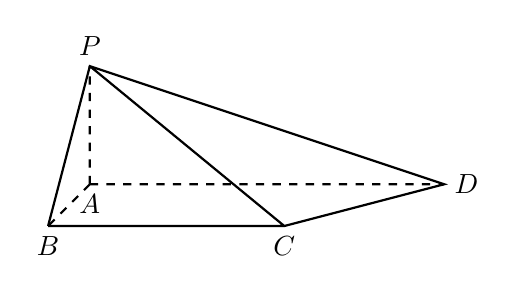
\begin{tikzpicture}[thick,scale = 1.5]
        \draw [dashed] (0,0) node [below] {$A$} -- (3,0) node [right] {$D$} (0,0) -- (225:0.5) node [below] {$B$} coordinate (B) (0,0) -- (0,1) node [above] {$P$};
        \draw (B) --++ (2,0) node [below] {$C$} coordinate (C) -- (3,0) -- (0,1) -- (B) (C) -- (0,1);
    \end{tikzpicture}
\end{center}
(1) 求异面直线$PB$与$CD$所成角的大小;\\
(2) 求四棱锥$P-ABCD$的体积.
\item 如图, 在直三棱柱$ABC-A_1B_1C_1$中, $\angle BAC=90^\circ$, $|AB|=|AC|=a$, $|AA_1|=2a$, $D$为$BC$的中点, $E$为$CC_1$上的点, 且$|CE|=\dfrac 14 |CC_1|$.
\begin{center}
    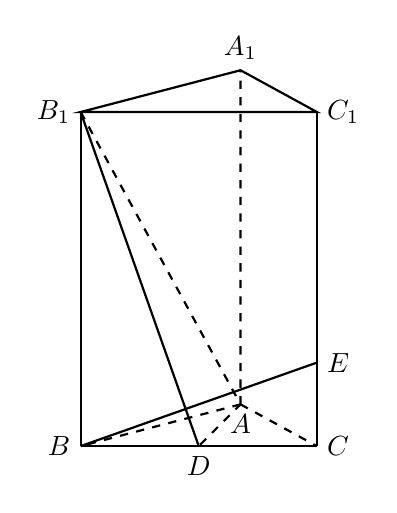
\begin{tikzpicture}[thick,scale = 1.5]
        \draw (0,0) node [left] {$B$} coordinate (B) -- (2,0) node [right] {$C$} coordinate (C);
        \draw [dashed] (1,0) ++ (45:0.5) node [below] {$A$} coordinate (A) -- (B) (A) -- (C) (A) --++ (0,{2*sqrt(2)}) node [above] {$A_1$} coordinate (A1);
        \draw (B) --++ (0,{2*sqrt(2)}) node [left] {$B_1$} coordinate (B1) (C) --++ (0,{2*sqrt(2)}) node [right] {$C_1$} coordinate (C1);
        \draw (A1) -- (B1) -- (C1) -- cycle;
        \draw [dashed] (B1) -- (A) -- (1,0) node [below] {$D$} coordinate (D);
        \draw (B1) -- (D) (C) ++ (0,{sqrt(2)/2}) node [right] {$E$} -- (B);
    \end{tikzpicture}
\end{center}
(1) 求证: $BE\perp \text{平面}ADB_1$;\\
(2) 求二面角$B-AB_1-D$的大小.
\item 在长方体$ABCD-A_1B_1C_1D_1$中, $|AB|=|BC|=2$, $A_1D$与$BC_1$所成的角为$\dfrac\pi 2$. 求$BC_1$与平面$BB_1D_1D$所成角的大小.
\item 如图, 在平行六面体$ABCD-A_1B_1C_1D_1$中, 点$E$、$F$分别在$B_1B$和$D_1D$上, 且$|BE|=\dfrac 13|BB_1|$, $|DF|=\dfrac 23|DD_1|$.
\begin{center}
    \begin{tikzpicture}[thick]
        \draw (0,0) node [below left] {$A$} coordinate (A) --++ (2,0) node [below right] {$B$} coordinate (B) --++ (45:{1.8/2}) node [right] {$C$} coordinate (C)
        --++ (0.2,2.6) node [above right] {$C_1$} coordinate (C1)
        --++ (-2,0) node [above left] {$D_1$} coordinate (D1) --++ (225:{1.8/2}) node [left] {$A_1$} coordinate (A1) -- cycle;
        \draw (A) ++ (2.2,2.6) node [below left] {$B_1$} coordinate (B1) -- (B) (B1) --++ (45:{1.8/2}) (B1) --++ (-2,0);
        \draw [dashed] (A) --++ (45:{1.8/2}) node [left] {$D$} coordinate (D) --++ (2,0) (D) --++ (0.2,2.6);
        \draw ($(B)!{1/3}!(B1)$) node [right] {$E$} coordinate (E) -- (C1) (E) -- (A);
        \draw [dashed] ($(D1)!{1/3}!(D)$) node [left] {$F$} coordinate (F) -- (E) (F) -- (C1) (F) -- (A);
    \end{tikzpicture}
\end{center}
(1) 求证: $A$、$E$、$C_1$、$F$四点共面;\\
(2) 若$\overrightarrow{EF} =\lambda \overrightarrow{AB}+ \mu \overrightarrow{AD}+ \nu \overrightarrow{AA_1}$, 求$\lambda+\mu+\nu$的值.
\item 如图, 在正方体$ABCD-A_1B_1C_1D_1$中, $E$、$F$分别是$BC$、$A_1D_1$的中点.
\begin{center}
    \begin{tikzpicture}[thick]
        \draw (0,0) node [below left] {$B$} coordinate (B) --++ (2,0) node [below right] {$C$} coordinate (C) --++ (45:{2/2}) node [right] {$D$} coordinate (D)
        --++ (0,2) node [above right] {$D_1$} coordinate (D1)
        --++ (-2,0) node [above left] {$A_1$} coordinate (A1) --++ (225:{2/2}) node [left] {$B_1$} coordinate (B1) -- cycle;
        \draw (A) ++ (2,2) node [right] {$C_1$} coordinate (C1) -- (C) (C1) --++ (45:{2/2}) (C1) --++ (-2,0);
        \draw [dashed] (A) --++ (45:{2/2}) node [left] {$A$} coordinate (A) --++ (2,0) (A) --++ (0,2);
        \draw [dashed] ($(B)!0.5!(C)$) node [below] {$E$} coordinate (E) -- (D) --  ($(D1)!0.5!(A1)$) node [above] {$F$} coordinate (F) (A1) -- (C);
        \draw (E) -- (B1) -- (F);
    \end{tikzpicture}
\end{center}
(1) 求证: 四边形$B_1EDF$是菱形;\\
(2) 求异面直线$A_1C$与$DE$所成角的大小.
\item 在正方体$ABCD-A_1B_1C_1D_1$中, $E$、$F$分别是$BC$、$CC_1$的中点.\\
(1) 求证: 点$D_1$在平面$AEF$上;\\
(2) 求平面$AEFD_1$与底面$ABCD$所成二面角的大小.
\item 如图, $ABCD-A_1B_1C_1D_1$为正方体, 动点$P$在对角线$BD_1$上, 记$\dfrac{|D_1P|}{|D_1B|}=\lambda$.
\begin{center}
    \begin{tikzpicture}[thick]
        \draw (0,0) node [below left] {$A$} coordinate (A) --++ (2,0) node [below right] {$B$} coordinate (B) --++ (45:{2/2}) node [right] {$C$} coordinate (C)
        --++ (0,2) node [above right] {$C_1$} coordinate (C1)
        --++ (-2,0) node [above left] {$D_1$} coordinate (D1) --++ (225:{2/2}) node [left] {$A_1$} coordinate (A1) -- cycle;
        \draw (A) ++ (2,2) node [right] {$B_1$} coordinate (B1) -- (B) (B1) --++ (45:{2/2}) (B1) --++ (-2,0);
        \draw [dashed] (A) --++ (45:{2/2}) node [left] {$D$} coordinate (D) --++ (2,0) (D) --++ (0,2);
        \draw (D1) -- (B1) -- (C);
        \draw [dashed] (B) -- (D1) (C) -- ($(B)!0.4!(D1)$) node [above] {$P$} -- (A);
    \end{tikzpicture}
\end{center}
(1) 求证: $AP\perp B_1C$;\\
(2) 若异面直线$AP$与$D_1B_1$所成角为$\dfrac \pi 4$, 求$\lambda$的值;\\
(3) 当$\angle APC$为钝角时, 求$\lambda$的取值范围.
\item 如图, 平行六面体$ABCD-A_1B_1C_1D_1$的底面$ABCD$是正方形, $O$为底面的中心, $A_1O\perp\text{平面}ABCD$, $|AB|=|AA_1|=\sqrt 2$.
\begin{center}
    \begin{tikzpicture}[thick,scale = 1.5]
        \draw (0,0) node [below left] {$A$} coordinate (A) --++ ({sqrt(2)},0) node [below right] {$B$} coordinate (B) --++ (45:{sqrt(2)/2}) node [right] {$C$} coordinate (C);
        \draw [dashed] (C) --++ ({-sqrt(2)},0) node [below] {$D$} coordinate (D) -- (A);
        \draw ($(A)!0.5!(C)$) node [below] {$O$} coordinate (O) ++ (0,1) node [left] {$A_1$} coordinate (A1) --++ ({sqrt(2)},0) node [above] {$B_1$} coordinate (B1) --++ (45:{sqrt(2)/2}) node [right] {$C_1$} coordinate (C1) --++ ({-sqrt(2)},0) node [above] {$D_1$} coordinate (D1) -- (A1); 
        \draw (A) -- (A1) (B) -- (B1) (C) -- (C1);
        \draw [dashed] (O) -- (A1) -- (D) (D1) -- (D) -- (B) (A) -- (C);
    \end{tikzpicture}
\end{center}
(1) 求证: $A_1C\perp \text{平面}BB_1D_1D$;\\
(2) 求平面$OCB_1$与平面$BB_1D_1D$所成二面角的大小.
\item 填空题:\\
(1) 已知数列$\{a_n\}$是等差数列, 下面的数列中必为等差数列的序号是\blank{50}.\\
\textcircled{1} $\{a_{2n}\}$ \textcircled{2} $\{a_n+a_{n+1}\}$ \textcircled{3} $\{3a_n+1\}$ \textcircled{4} $\{|a_n|\}$\\
(2) 已知数列$\{a_n\}$是等比数列, 下面的数列中必为等比数列的序号是\blank{50}.\\
\textcircled{1} $\{a_n^2\}$ \textcircled{2} $\{a_n+a_{n+1}\}$ \textcircled{3} $\{\dfrac 1{a_n}\}$ \textcircled{4} $\{2^{a_n}\}$
\item 选择题:\\
(1) 我国古代数学名著《算法统宗》中有如下问题: ``远望巍巍塔七层, 红光点点倍加增, 共灯三百八十一, 请问尖头几盏灯?''意思是: 一座$7$层塔共挂了$381$盏灯, 且相邻两层中的下一层灯的盏数是上一层灯的盏数的$2$倍, 则塔的顶层灯的盏数是\bracket{20}.
\fourch{$1$}{$3$}{$5$}{$9$}
(2) 已知数列$\{a_n\}$, 若$a_1=3$, $a_2=6$, 且$a_{n+2}=a_{n+1}-a_n$($n$为正整数), 则数列的第$35$项为\bracket{20}.
\fourch{$6$}{$-3$}{$-12$}{$-6$}
\item 在等差数列$\{a_n\}$中, 已知公差$d=\dfrac12$, 且$a_1+a_3+a_5+\cdots+a_{99}=60$. 求$a_1+a_2+a_3+\cdots+a_{99}+a_{100}$的值.
\item 已知存在常数$t$, 使得等差数列$\{a_n\}$的前$n$项和为$S_n=tn^2+(t-9)n+t-\dfrac 32$. 求该数列$\{a_n\}$的通项公式.
\item 设$S_n$为等差数列$\{a_n\}$的前$n$项和, 求证: 数列$\{\dfrac{S_n}n\}$是等差数列.
\item 已知数列$\{\log_3a_n\}$是等差数列, 且$\log_3a_1+\log_3a_2+\cdots+\log_3a_{10}=10$. 求$a_5a_6$.
\item 已知等差数列$\{a_n\}$的前$n$项和为$S_n$, 且满足$a_1=29$, $S_{10}=S_{20}$. 这个数列的前多少项和最大? 并求此最大值.
\item 在$2$与$9$之间插入两个数, 使前三个数成等差数列, 后三个数成等比数列. 试写出这个数列.
\item 已知数列$\{a_n\}$是等比数列, 且$a_1$, $a_2$, $a_4$成等差数列. 求数列$\{a_n\}$的公比.
\item 用数学归纳法证明: $\dfrac12+\dfrac2{2^2}+\dfrac3{2^3}+\cdots+\dfrac n{2^n}=2-\dfrac{n+2}{2^n}$($n$为正整数).
\item (1) 依次计算下列各式的值: $\dfrac11,\dfrac11+\dfrac1{1+2},\dfrac11+\dfrac1{1+2}+\dfrac1{1+2+3},\dfrac11+\dfrac1{1+2}+\dfrac1{1+2+3}+\dfrac1{1+2+3+4}$.\\
(2) 根据(1)中的计算结果, 猜想$S_n=\dfrac11+\dfrac1{1+2}+\dfrac1{1+2+3}+\cdots+\dfrac1{1+2+3+\cdots+n}$($n$为正整数)的表达式, 并用数学归纳法证明相应的结论.
\item 选择题:\\
(1) 已知$a, x, b$和$b, y, c$均为等差数列, 而$a, b, c$为等比数列, 且$xy\ne 0$, 则$\dfrac{a}{x}+\dfrac{c}{y}$的值等于\bracket{20}.
\fourch{$1$}{$2$}{$3$}{$4$}
(2) 已知两个等差数列$\{a_n\}$和$\{b_n\}$的前$n$项和分别为$A_n$和$B_n$, 且满足$\dfrac{A_n}{B_n}=\dfrac{7n+45}{n+3}$, 则使得$\dfrac{a_n}{b_n}$为整数的正整数$n$的个数为\bracket{20}.
\fourch{$2$}{$3$}{$4$}{$5$}
\item 已知$S_n$是等比数列$\{a_n\}$的前$n$项和, 且$S_3$, $S_9$, $S_6$成等差数列. 求证: $a_2$, $a_8$, $a_5$成等差数列.
\item 已知在等差数列$\{a_n\}$中, $a_{10}=0$.\\
(1) 求证: $a_1+a_2+\cdots+a_n=a_1+a_2+\cdots+a_{19-n}$对一切小于$19$的正整数$n$都成立;\\
(2) 类比上述性质, 在等比数列$\{b_n\}$中, 若$b_9=1$, 可以得到什么结论?
\item 已知数列$\{a_n\}$的各项均为正数, $a_1=\dfrac 13$, 且$a_n=\dfrac{a_{n-1}}{2a_{n-1}+1} \ (n\ge 2)$.\\
(1) 求证: 数列$\{\dfrac 1{a_n}\}$是等差数列;\\
(2) 若数列$\{b_n\}$满足$b_n=\begin{cases}2, & n=1,\\ na_n, & n \ge 2,\end{cases}$ 求数列$\{b_n\}$中的最大项与最小项.
\item 已知数列$\{a_n\}$的前$n$项和为$S_n$, 且$S_n=\dfrac{n(a_1+a_n)}2$. 求证: 数列$\{a_n\}$为等差数列.
\item 用数学归纳法证明: $1-\dfrac12+\dfrac 13-\dfrac 14+\cdots +\dfrac{1}{2n-1}-\dfrac{1}{2n}=\dfrac{1}{n+1}+\dfrac{1}{n+2}+\cdots+\dfrac{1}{2n}$($n$为正整数).
\item 是否存在常数$a$、$b$、$c$, 使等式$1\cdot (n^2-1^2)+2\cdot (n^2-2^2)+\cdots +n\cdot (n^2-n^2)=an^4+bn^2+c$对任意正整数$n$都成立? 证明你的结论.
\item 如图所示, 有三根直杆和套在一根直杆上的若干金属片, 把金属片按下列规则从一根直杆上全部移到另一根直杆上:\\
\textcircled{1} 每次只移动1个金属片;\\
\textcircled{2} 较大的金属片不能放在较小的金属片上面.
\begin{center}
    \begin{tikzpicture}[thick]
        \draw (0.4,0) rectangle (0.6,3) (2.9,0) rectangle (3.1,3) (-2.1,0.8) rectangle (-1.9,3);
        \draw (-2.5,0.8) rectangle (-1.5,0.6) (-2.7,0.6) rectangle (-1.3,0.4) (-2.9,0.4) rectangle (-1.1,0.2) (-3.1,0.2) rectangle(-0.9,0);
        \draw (-2,3) node [above] {$1$} (0.5,3) node [above] {$2$} (3,3) node [above] {$3$};
    \end{tikzpicture}
\end{center}
试推测: 把$n$个金属片从$1$号直杆移到$3$号直杆, 最少需要移动多少次?
\item 如图, 将一个边长为$1$的正三角形的每条边三等分, 以中间一段为边向外作正三角形, 并擦去中间这一段, 如此继续下去得到的曲线称为科克雪花曲线. 将下面的图形依次记作$M_1$、$M_2$、$M_3$、$\cdots$、$M_n$、$\cdots$.
\begin{center}
    \begin{tikzpicture}[scale = 2,thick]
        \draw (0,0) ++ (90:{1/sqrt(3)}) coordinate (A1) (0,0) ++ (210:{1/sqrt(3)}) coordinate (B1) (0,0) ++ (-30:{1/sqrt(3)}) coordinate (C1);
        \draw (A1) -- (B1) -- (C1) -- cycle;
        \draw (0,-1) node {$M_1$};
        \draw (B1) ++ (1.5,0) coordinate (B2) --++ (0:{1/3}) --++ (-60:{1/3}) --++ (60:{1/3}) --++ (0:{1/3}) --++ (120:{1/3}) --++ (60:{1/3}) --++ (180:{1/3}) --++ (120:{1/3}) --++ (240:{1/3}) --++ (180:{1/3}) --++ (-60:{1/3}) --++ (-120:{1/3});
        \draw (1.5,-1) node {$M_2$};
        \draw (B2) ++ (1.5,0) coordinate (B3) --++ (0:{1/9}) --++ (-60:{1/9}) --++ (60:{1/9}) --++ (0:{1/9}) --++ (-60:{1/9})--++ (-120:{1/9}) --++ (0:{1/9}) --++ (-60:{1/9}) --++ (60:{1/9}) --++ (0:{1/9}) --++ (120:{1/9}) --++ (60:{1/9}) --++ (0:{1/9}) --++ (-60:{1/9}) --++ (60:{1/9}) --++ (0:{1/9}) --++ (120:{1/9}) --++ (60:{1/9}) --++ (180:{1/9}) --++ (120:{1/9}) --++ (60:{1/9})--++ (0:{1/9}) --++ (120:{1/9}) --++ (60:{1/9}) --++ (180:{1/9}) --++ (120:{1/9}) --++ (240:{1/9}) --++ (180:{1/9}) --++ (120:{1/9}) --++ (60:{1/9}) --++ (180:{1/9}) --++ (120:{1/9}) --++ (-120:{1/9}) --++ (-180:{1/9}) --++ (-60:{1/9}) --++ (-120:{1/9}) --++ (-180:{1/9})--++ (-240:{1/9}) --++ (-120:{1/9}) --++ (-180:{1/9}) --++ (-60:{1/9}) --++ (-120:{1/9}) --++ (0:{1/9}) --++ (-60:{1/9}) --++ (-120:{1/9}) --++ (-180:{1/9}) --++ (-60:{1/9}) --++ (-120:{1/9});
        \draw (3,-1) node {$M_3$};
        \draw (4.5,-1) node {$\cdots$} (4.5,0) node {$\cdots$};
    \end{tikzpicture}
\end{center}
(1) 求$M_n$的周长;\\
(2) 求$M_n$的面积;\\
(3) 当$n\to +\infty$时, 科克雪花曲线所围成的图形是周长无限增大而面积却有极限的图形吗? 若是, 请求出其面积的极限; 若不是, 请说明理由.
\item 若``$a>b$'', 则``$a^3>b^3$''是\blank{50}命题(填: 真、假).
\item 已知$A=(-\infty ,0]$, $B=(a,+\infty )$, 若$A\cup B=\mathbf{R}$, 则$a$的取值范围是\blank{50}.
\item $z+2\bar{z}=9+4\mathrm{i}$($\mathrm{i}$为虚数单位), 则$|z|=$\blank{50}.
\item 若$\triangle ABC$中, $a+b=4$, $\angle C=30^\circ$, 则$\triangle ABC$面积的最大值是\blank{50}.
\item 若函数$f(x)=\log_2\dfrac{x-a}{x+1}$的反函数的图像过点$(-2,3)$, 则$a=$\blank{50}.
\item 若半径为2的球$O$表面上一点$A$作球$O$的截面, 若$OA$与该截面所成的角是$60^\circ$, 则该
截面的面积是\blank{50}.
\item 抛掷一枚均匀的骰子(刻有1、2、3、4、5、6)三次, 得到的数字依次记作$a$、$b$、$c$, 则$a+b\mathrm{i}$($\mathrm{i}$为虚数单位)是方程$x^2-2x+c=0$的根的概率是\blank{50}.
\item 设常数$a>0$, $(x+\dfrac{a}{\sqrt{x}})^9$展开式中$x^6$的系数为$4$, 则$\displaystyle\lim_{n\to \infty}(a+a^2+\cdots+a^n)=$\blank{50}.
\item 已知直线$l$经过点$(-\sqrt{5},0)$且方向向量为$(2,-1)$, 则原点$O$到直线$l$的距离为\blank{50}.
\item 若双曲线的一条渐近线为$x+2y=0$, 且双曲线与抛物线$y=x^2$的准线仅有一个公共点, 则此双曲线的标准方程为\blank{50}.
\item $\displaystyle\lim_{n\to \infty}\dfrac{2n-5}{n+1}=$\blank{50}.
\item 已知抛物线$C$的顶点在平面直角坐标系原点, 焦点在$x$轴上, 若$C$经过点$M(1,3)$, 则其焦点到准线的距离为\blank{50}.
\item 若线性方程组的增广矩阵为$\begin{pmatrix}    a & 0 & 2 \\ 0 & 1 & b\end{pmatrix}$, 解为$\begin{cases}    x=2, \\ y=1.\end{cases}$ 则$a+b=$\blank{50}.
\item 若复数$z$满足: $\mathrm{i}\cdot z=\sqrt{3}+\mathrm{i}$($\mathrm{i}$是虚数单位), 则$|z|=$\blank{50}.
\item 在$(x+\dfrac{2}{x^2})^6$的二项展开式中第四项的系数是\blank{50}(结果用数值表示).
\item 在长方体$ABCD-A_1B_1C_1D_1$中, 若$AB=BC=1$, $AA_1=\sqrt{2}$, 则异面直线$BD_1$与$CC_1$所成角的大小为\blank{50}.
\item 若函数$f(x)=\begin{cases}    2^x, & x\le 0, \\ -x^2+m, & x>0 \end{cases}$的值域为$(-\infty ,1]$, 则实数$m$的取值范围是\blank{50}.
\item 如图, 在$\triangle ABC$中, 若$AB=AC=3$, $\cos \angle BAC=\dfrac{1}{2}$, $\overrightarrow{DC}=2\overrightarrow{BD}$, 则$\overrightarrow{AD}\cdot \overrightarrow{BC}=$\blank{50}.
\begin{center}
    \begin{tikzpicture}[>=latex]
        \draw (0,0) node [left] {$B$} -- (3,0) node [right] {$C$} -- (1.5,{1.5*sqrt(3)}) node [above] {$A$} coordinate (A) -- cycle;
        \draw [->] (A) -- (1,0) node [below] {$D$};
    \end{tikzpicture}
\end{center}
\item 定义在$\mathbf{R}$上的偶函数$y=f(x)$, 当$x\ge 0$时, $f(x)=\lg (x^2-3x+3)$, 则$f(x)$在$\mathbf{R}$上的零点个数为\blank{50}个.
\item 将$6$辆不同的小汽车和$2$辆不同的卡车驶入如图所示的$10$个车位中的某$8$个内, 其中$2$辆卡车必须停在$A$与$B$的位置, 那么不同的停车位置安排共有\blank{50}种(结果用数值表示).
\begin{center}
    \begin{tikzpicture}[>=latex]
        \draw (0,0) node {$B$};
        \draw (0,1.2) node {$A$};
        \foreach \i in {-0.3,0.3,0.9,1.5}{\draw (-0.3,\i) -- (2.7,\i);};
        \foreach \i in {-0.3,0.3,...,2.8}{\draw (\i,-0.3) -- (\i, 0.3) (\i, 0.9) -- (\i, 1.5);};
    \end{tikzpicture}
\end{center}
\item 设集合$A=\{x||x-2|<1,x\in \mathbf{R}\}$, 集合$B=\mathbf{Z}$, 则$A\cap B=$\blank{50}.
\item 函数$y=\sin (\omega x-\dfrac{\pi}{3})$($\omega >0$)的最小正周期是$\pi$, 则$\omega =$\blank{50}.
\item 设$\mathrm{i}$为虚数单位, 在复平面上, 复数$\dfrac{3}{(2-\mathrm{i})^2}$对应的点到原点的距离为\blank{50}.
\item 若函数$f(x)=\log_2 (x+1)+a$的反函数的图像经过点$(4,1)$, 则实数$a=$\blank{50}.
\item 已知$(a+3b)^n$的展开式中, 各项系数的和与各项二项式系数的和之比为$64$, 则$n=$\blank{50}.
\item 甲、乙两人从$5$门不同的选修课中各选修$2$门, 则甲、乙所选的课程中恰有$1$门相同的选法有\blank{50}种.
\item 若圆锥的侧面展开图是半径为2$\text{cm}$, 圆心角为$270^\circ$的扇形, 则这个圆锥的体积为\blank{50}$\text{cm}^3$.
\item 若数列$\{a_n\}$的所有项都是正数, 且$\sqrt{a_1}+\sqrt{a_2}+\cdots +\sqrt{a_n}=n^2+3n$($n\in \mathbf{N}^*$), 则$\displaystyle\lim_{n\to\infty}\dfrac{1}{n^2}(\dfrac{a_1}{2}+\dfrac{a_2}{3}+\cdots +\dfrac{a_n}{n+1})=$\blank{50}.
\item 如图, 在$\triangle ABC$中, $\angle B=45^\circ$, $D$是$BC$边上的一点, $AD=5$, $AC=7$, $DC=3$, 则$AB$的长为\blank{50}.
\begin{center}
    \begin{tikzpicture}[scale = 0.5]
        \draw  (-6.830127018922193,0.)-- (3.,0.) node [below right] {$C$};
        \draw  (3.,0.)-- (-2.5,4.330127018922193) node [above] {$A$};
        \draw  (-2.5,4.330127018922193)-- (-6.830127018922193,0.) node [below left] {$B$};
        \draw  (-2.5,4.330127018922193)-- (0.,0.) node [below] {$D$};
    \end{tikzpicture}
\end{center}
\item 有以下命题:\\
\textcircled{1} 若函数$f(x)$既是奇函数又是偶函数, 则$f(x)$的值域为$\{0\}$; \\
\textcircled{2} 若函数$f(x)$是偶函数, 则$f(|x|)=f(x)$;\\
\textcircled{3} 若函数$f(x)$在其定义域内不是单调函数, 则$f(x)$不存在反函数;\\
\textcircled{4} 若函数$f(x)$存在反函数${{f}^{-1}}(x)$, 且${{f}^{-1}}(x)$与$f(x)$不完全相同, 则$f(x)$与${{f}^{-1}}(x)$图像的公共点必在直线$y=x$上; \\
其中真命题的序号是\blank{50}(写出所有真命题的序号).
\item 若集合$A=\{x|y^2=x,y\in \mathbf{R}\}$, $B=\{y|y=\sin x,x\in \mathbf{R}\}$, 则$A\cap B=$\blank{50}.
\item 若$-\dfrac{\pi}{2}<\alpha <\dfrac{\pi}{2}$, $\sin \alpha =\dfrac{3}{5}$, 则$\cot 2\alpha =$\blank{50}.
\item 函数$f(x)=1+\log_2 x$($x\ge 1$)的反函数$f^{-1}(x)=$\blank{50}.
\item 若$(1+x)^5=a_0+a_1x+a_2x^2+\cdots+a_5x^5$, 则$a_1+a_2+\cdots+a_5=$\blank{50}.
\item 设$k\in \mathbf{R}$, $\dfrac{y^2}{k}-\dfrac{x^2}{k-2}=1$表示焦点在$y$轴上的双曲线, 则半焦距的取值范围是\blank{50}.
\item 设$m\in \mathbf{R}$, 若$f(x)=(m+1)x^{\tfrac{2}{3}}+mx+1$是偶函数, 则$f(x)$的单调递增区间是\blank{50}.
\item 方程$\log_2(9^x-5)=2+\log_2(3^x-2)$的解$x=$\blank{50}.
\item 已知圆$C:x^2+y^2+2kx+2y+k^2=0$($k\in \mathbf{R}$)和定点$P(1,-1)$, 若过$P$可以作两条直线与圆$C$相切, 则$k$的取值范围是\blank{50}.
\item 如图, 在直三棱柱$ABC-A_1B_1C_1$中, $\angle ABC=90^\circ$, $AB=BC=1$, 若$A_1C$与平面$B_1BCC_1$所成的角为$\dfrac{\pi}{6}$, 则三棱锥$A_1-ABC$的体积为\blank{50}.
\begin{center}
    \begin{tikzpicture}[scale = 1.5]
        \draw [dashed] (0,0) -- (1,0) node [right] {$C$} coordinate (C) (0,0) -- (225:0.5) node [below left] {$A$} coordinate (A) (0,0) node [left] {$B$} coordinate (B) -- (0,{sqrt(2)}) node [above left] {$B_1$} coordinate (B1);
        \draw (A) --+ (0,{sqrt(2)}) node [left] {$A_1$} coordinate (A1);
        \draw (C) --+ (0,{sqrt(2)}) node [above right] {$C_1$} coordinate (C1);
        \draw (A1) -- (B1) -- (C1) -- (A1) -- (C) -- (A);
    \end{tikzpicture}
\end{center}
\item 设地球半径为$R$, 若$A$、$B$两地均位于北纬$45^\circ$, 且两地所在纬度圈上的弧长为$\dfrac{\sqrt{2}}{4}\pi R$, 则$A$、$B$之间的球面距离是\blank{50}(结果用含有$R$的代数式表示).
\item 复数$\mathrm{i}(2+\mathrm{i})$的虚部为\blank{50}.
\item 设函数$f(x)=\begin{cases}\log_2 x, & x>0, \\ 4^x, & x\le 0,\end{cases}$ 则$f(f(-1))=$\blank{50}.
\item 已知$M=\{x||x-1|\le 2,x\in \mathbf{R}\}$, $P=\{x|\dfrac{1-x}{x+2}\ge 0,x\in \mathbf{R}\}$, 则$M\cap P=$\blank{50}.
\item 抛物线$y=x^2$上一点$M$到焦点的距离为$1$, 则点$M$的纵坐标为\blank{50}.
\item 已知无穷数列$\{a_n\}$满足$a_{n+1}=\dfrac12{a_n}$($n\in \mathbf{N}^*$), 且$a_2=1$, 记$S_n$为数列$\{a_n\}$的前$n$项和, 则$\displaystyle\lim_{n\to \infty}S_n=$\blank{50}.
\item 已知$x,y\in \mathbf{R}^+$, 且$x+2y=1$, 则$xy$的最大值为\blank{50}.
\item 已知圆锥的母线$l=10$, 母线与旋转轴的夹角$\alpha =30^\circ$, 则圆锥的表面积为\blank{50}.
\item 若$(2x^2+\dfrac1x)^n$($n\in \mathbf{N}^*$)的二项展开式中的第$9$项是常数项, 则$n=$\blank{50}.
\item 已知$A,B$分别是函数$f(x)=2\sin \omega x$($\omega >0$)在$y$轴右侧图像上的第一个最高点和第一个最低点, 且$\angle AOB=\dfrac\pi 2$, 则该函数的最小正周期是\blank{50}.
\item 将序号分别为1、2、3、4、5的$5$张参观券全部分给$4$人, 每人至少一张, 如果分给同一人的$2$张参观券连号, 那么不同的分法种数是\blank{50}.
\item $\displaystyle\lim_{n\to\infty}\dfrac{2n+3}{n+1}=$\blank{50}.
\item 设全集$U=\mathbf{R}$, 集合$A=\{-1,0,1,2,3\}$, $B=\{x|x\ge 2\}$, 则$A\cap {\complement_U}B=$\blank{50}.
\item 不等式$\dfrac{x+1}{x+2}<0$的解集为\blank{50}.
\item 椭圆$\begin{cases} x=5\cos \theta,  \\ y=4\sin \theta  \end{cases}$($\theta$为参数)的焦距为\blank{50}.
\item 若函数$y=\begin{vmatrix}   \cos x & \sin x  \\   \sin x & \cos x  \\ \end{vmatrix}$的最小正周期为$a\pi $, 则实数$a$的值为\blank{50}.
\item 若点$(8,4)$在函数$f(x)=1+\log_a x$图像上, 则$f(x)$的反函数为\blank{50}.
\item 已知向量$\overrightarrow{a}=(1,2)$, $\overrightarrow{b}=(0,3)$, 则$\overrightarrow{b}$在$\overrightarrow{a}$的方向上的投影为\blank{50}.
\item 已知一个底面置于水平面上的圆锥, 其左视图是边长为6的正三角形, 则该圆锥的侧面积为\blank{50}.
\item 某班级要从$5$名男生和$2$名女生中选出$3$人参加公益活动, 则在选出的$3$人中男、女生
均有的概率为\blank{50}(结果用最简分数表示).
\item 设常数$a>0$, 若$(x+\dfrac ax)^9$的二项展开式中$x^5$的系数为$144$, 则$a=$\blank{50}.
\item 设集合$M=\{x|x^2=x\}$, $N=\{x|\lg x\le 0\}$, 则$M\cap N=$\blank{50}.
\item 已知$a$、$b\in \mathbf{R}$, $\mathrm{i}$是虚数单位, 若$a+\mathrm{i}=2-b\mathrm{i}$, 则$(a+b\mathrm{i})^2=$\blank{50}.
\item 已知函数$f(x)=a^x-1$的图像经过$(1,1)$点, 则$f^{-1}(3)=$\blank{50}.
\item 不等式$x|x-1|>0$的解集为\blank{50}.
\item 已知$\overrightarrow a=(\sin x,\cos x)$, $\overrightarrow b=(\sin x,\sin x)$, 则函数$f(x)=\overrightarrow a\cdot \overrightarrow b$的最小正周期为\blank{50}.
\item 里约奥运会游泳小组赛采用抽签方法决定运动员比赛的泳道, 在由$2$名中国运动员和$6$名外国运动员组成的小组中, $2$名中国运动员恰好抽在相邻泳道的概率为\blank{50}.
\item 如图, 在棱长为$1$的正方体$ABCD-A_1B_1C_1D_1$中, 点$P$在截面$A_1DB$上, 则线段$AP$的最小值为\blank{50}.
\begin{center}
    \begin{tikzpicture}
        \draw (0,0) node [below left] {$A$} coordinate (A) --++ (2,0) node [below right] {$B$} coordinate (B) --++ (45:{2/2}) node [right] {$C$} coordinate (C)
        --++ (0,2) node [above right] {$C_1$} coordinate (C1)
        --++ (-2,0) node [above left] {$D_1$} coordinate (D1) --++ (225:{2/2}) node [left] {$A_1$} coordinate (A1) -- cycle;
        \draw (A) ++ (2,2) node [right] {$B_1$} coordinate (B1) -- (B) (B1) --++ (45:{2/2}) (B1) --++ (-2,0);
        \draw [dashed] (A) --++ (45:{2/2}) node [left] {$D$} coordinate (D) --++ (2,0) (D) --++ (0,2);
        \draw (A1) -- (B);
        \draw [dashed] (B) -- (D) -- (A1);
    \end{tikzpicture}
\end{center}
\item 设$(1+x)^n=a_0+a_1x+a_2x^2+a_3x^3+\cdots +a_nx^n$, 若$\dfrac{a_2}{a_3}=\dfrac13$, 则$n=$\blank{50}.
\item 已知圆锥底面半径与球的半径都是$1\text{cm}$, 如果圆锥的体积与球的体积恰好也相等, 那么这个圆锥的侧面积是\blank{50}$\text{cm}^2$.
\item 设$P(x,y)$是曲线$C:\sqrt{\dfrac{x^2}{25}}+\sqrt{\dfrac{y^2}9}=1$上的点, $F_1(-4,0)$, $F_2(4,0)$, 则$|PF_1|+|PF_2|$的最大值为\blank{50}.
\item 已知复数$z=2+\mathrm{i}$($\mathrm{i}$为虚数单位), 则$\overline{{z^2}}=$\blank{50}.
\item 已知集合$A=\{x|\dfrac12\le {2^x}<16\}$, $B=\{x|y=\log _2(9-x^2)\}$, 则$A\cap B=$\blank{50}.
\item 在二项式$(x+\dfrac2x)^6$的展开式中, 常数项是\blank{50}.
\item 等轴双曲线$x^2-y^2=a^2$与抛物线$y^2=16x$的准线交于$A$、$B$两点, 且$|AB|=4\sqrt3$, 则该双曲线的实轴长等于\blank{50}.
\item 若由矩阵$\begin{pmatrix}a & 2 \\ 2 & a\end{pmatrix}\begin{pmatrix}x \\ y\end{pmatrix}=\begin{pmatrix}a+2 \\ 2a\end{pmatrix}$表示$x$、$y$的二元一次方程组无解, 则实数$a=$\blank{50}.
\item 已知$f(x)=\sin\dfrac\pi 3x$, $A=\{1,2,3,4,5,6,7,8\}$, 现从集合$A$中任取两个不同元素$s$、$t$, 则使得$f(s)\cdot f(t)=0$发生的概率是\blank{50}.
\item 若圆锥侧面积为$20\pi$, 且母线与底面所成角为$\arccos \dfrac45$, 则该圆锥的体积为\blank{50}.
\item 已知数列$\{a_n\}$的通项公式为$a_n=n^2+bn$, 若数列$\{a_n\}$是单调递增数列, 则实数$b$的取值范围是\blank{50}.
\item 将边长为$10$的正三角形$ABC$, 按``斜二测''画法在水平放置的平面上画出为$\triangle A'B'C'$, 则$\triangle A'B'C'$中最短边的边长为\blank{50}(精确到0.01).
\item 已知点$A$是圆$O: x^2+y^2=4$上的一个定点, 点$B$是圆$O$上的一个动点, 若满足$|\overrightarrow{AO}+\overrightarrow{BO}|=|\overrightarrow{AO}-\overrightarrow{BO}|$, 则$\overrightarrow{AO}\cdot \overrightarrow{AB}=$\blank{50}.
\item 方程$\lg (3x+4)=1$的解$x=$\blank{50}.
\item 若关于$x$的不等式$\dfrac{x-a}{x-b}>0$($a,b\in \mathbf{R}$)的解集为$(-\infty ,1)\cup (4,+\infty)$, 则$a+b=$\blank{50}.
\item 已知数列$\{a_n\}$的前$n$项和为$S_n=2^n-1$, 则此数列的通项公式为\blank{50}.
\item 函数$f(x)=\sqrt x+1$的反函数是\blank{50}.
\item $(1+2x)^6$展开式中$x^3$项的系数为\blank{50}(用数字作答).
\item 如图, 已知正方形$ABCD-A_1B_1C_1D_1$, $AA_1=2$, $E$为棱$CC_1$的中点, 则三棱锥$D_1-ADE$的体积为\blank{50}.
\begin{center}
    \begin{tikzpicture}
        \draw (0,0) node [below left] {$A$} coordinate (A) --++ (2,0) node [below right] {$B$} coordinate (B) --++ (45:{2/2}) node [right] {$C$} coordinate (C)
        --++ (0,2) node [above right] {$C_1$} coordinate (C1)
        --++ (-2,0) node [above left] {$D_1$} coordinate (D1) --++ (225:{2/2}) node [left] {$A_1$} coordinate (A1) -- cycle;
        \draw (A) ++ (2,2) node [right] {$B_1$} coordinate (B1) -- (B) (B1) --++ (45:{2/2}) (B1) --++ (-2,0);
        \draw [dashed] (A) --++ (45:{2/2}) node [left] {$D$} coordinate (D) --++ (2,0) (D) --++ (0,2);
        \draw ($ (C)!0.5!(C1) $) node [right] {$E$} coordinate (E);
        \draw [dashed] (E) -- (D1) -- (A) -- (E) -- (D);
    \end{tikzpicture}
\end{center}
\item 从单词``shadow''中任意选取$4$个不同的字母排成一排, 则其中含有``a''的共有\blank{50}种排法(用数字作答).
\item 集合$\{x|\cos (\pi \cos x)=0,x\in [0,\pi]\}=$\blank{50}(用列举法表示).
\item 如图, 已知半径为1的扇形$AOB$, $\angle AOB=60^\circ$, $P$为弧$\overset\frown{AB}$上的一个动点, 则$\overrightarrow{OP}\cdot \overrightarrow{AB}$取值范围是\blank{50}.
\begin{center}
    \begin{tikzpicture}[>=latex,scale = 1.3]
        \draw (0,0) node [below left] {$O$} -- (2,0) node [below right] {$B$} (0,0) -- (1,{sqrt(3)}) node [above] {$A$} -- cycle;
        \draw (2,0) arc (0:60:2);
        \draw [->] (0,0) -- (25:2) node [above right] {$P$};
        \draw [->] (1,{sqrt(3)}) -- (2,0);
    \end{tikzpicture}
\end{center}
\item 已知$x$、$y$满足曲线方程$x^2+\dfrac1{y^2}=2$, 则$x^2+y^2$的取值范围是\blank{50}.
\item 已知$U=\mathbf{R}$, 集合$A=\{x|4-2x\ge x+1\}$, 则${\complement_U}A=$\blank{50}.
\item 三阶行列式$\begin{vmatrix}   3 & -5 & 1 \\   2 & 3 & -6 \\   -7 & 2 & 4 \\ \end{vmatrix}$中元素$-5$的代数余子式的值为\blank{50}.
\item $(1-\dfrac x2)^8$的二项展开式中含$x^2$项的系数是\blank{50}.
\item 已知一个球的表面积为$16\pi$, 则它的体积为\blank{50}.
\item 一个袋子中共有$6$个球, 其中$4$个红色球, $2$个蓝色球, 这些球的质地和形状一样, 从中任意抽取$2$个球, 则所抽的球都是红色球的概率是\blank{50}.
\item 已知直线$l:x-y+b=0$被圆$C:x^2+y^2=25$所截得的弦长为$6$, 则$b=$\blank{50}.
\item 若复数$(1+a\mathrm{i})(2-\mathrm{i})$在复平面上所对应的点在直线$y=x$上, 则实数$a=$\blank{50}.
\item 函数$f(x)=(\sqrt3\sin x+\cos x)(\sqrt3\cos x-\sin x)$的最小正周期为\blank{50}.
\item 过双曲线$C:\dfrac{x^2}{a^2}-\dfrac{y^2}4=1$的右焦点$F$作一条垂直于$x$轴的垂线交双曲线$C$的两条渐近线于$A$、$B$两点, $O$为坐标原点, 则$\triangle OAB$的面积的最小值为\blank{50}.
\item 若关于$x$的不等式$|2^x-m|-\dfrac1{2^x}<0$在区间$[0,1]$内恒成立, 则实数$m$的范围\blank{50}.
\item 已知集合$A=\{1,2,4,6,8\}$, $B=\{x|x=2k,k\in A\}$, 则$A\cap B=$\blank{50}.
\item 已知$\dfrac{\overline z}{1-\mathrm{i}}=2+\mathrm{i}$, 则复数$z$的虚部为\blank{50}.
\item 设函数$f(x)=\sin x-\cos x$, 且$f(a)=1$, 则$\sin 2a=$\blank{50}.
\item 已知二元一次方程$\begin{cases} {a_1}x+{b_1}y={c_1}, \\  {a_2}x+{b_2}y={c_2} \end{cases}$的增广矩阵是$\begin{pmatrix} 1 & -1 & 1 \\  1 & 1 & 3 \\ \end{pmatrix}$, 则此方程组的解是\blank{50}.
\item 数列$\{a_n\}$是首项为$1$, 公差为$2$的等差数列, $S_n$是它前$n$项和, 则$\displaystyle\lim_{n\to\infty}\dfrac{S_n}{a_n^2}=$\blank{50}.
\item 已知角$A$是$\triangle ABC$的内角, 则``$\cos A=\dfrac12$''是``$\sin A=\dfrac{\sqrt3}2$''的\blank{50}条件(填``充分非必要''、``必要非充分''、``充要条件''、``既非充分又非必要''之一).
\item 若双曲线$x^2-\dfrac{y^2}{b^2}=1$的一个焦点到其渐近线距离为$2\sqrt2$, 则该双曲线焦距等于\blank{50}.
\item 若正项等比数列$\{a_n\}$满足: $a_3+a_5=4$, 则$a_4$的最大值为\blank{50}.
\item 已知函数$f(x)=\sin (2x+\dfrac\pi 3)$在区间$[0,a]$(其中$a>0$)上单调递增, 则实数$a$的取值范围是\blank{50}.
\item 设函数$f(x)=\begin{cases}    x^6, & x\ge 1,  \\   -2x-1, & x\le -1, \end{cases}$ 则当$x\le -1$时, $f[f(x)]$表达式的展开式中含${x^2}$项的系数是\blank{50}.
\item ``$x<0$''是``$x<a$''的充分非必要条件, 则$a$的取值范围是\blank{50}.
\item 函数$f(x)=1-3\sin ^2(x+\dfrac\pi 4)$的最小正周期为\blank{50}.
\item 若复数$z$为纯虚数, 且满足$(2-\mathrm{i})z=a+\mathrm{i}$($\mathrm{i}$为虚数单位), 则实数$a$的值为\blank{50}.
\item 二项式$(x^2+\dfrac 1x)^5$的展开式中, $x$的系数为\blank{50}.
\item 用半径$1$米的半圆形薄铁皮制作圆锥型无盖容器, 其容积为\blank{50}立方米.
\item 已知$\alpha$为锐角, 且$\cos (\alpha +\dfrac\pi 4)=\dfrac35$, 则$\sin \alpha =$\blank{50}.
\item 已知正四棱柱$ABCD-A_1B_1C_1D_1$, $AB=a$, $AA_1=2a$, $E$、$F$分别是棱$AD$、$CD$的中点,则异面直线$BC_1$与$EF$所成角是\blank{50}.
\item 在无穷等比数列$\{a_n\}$中, $\displaystyle\lim_{n\to\infty}(a_1+a_2+\cdots+a_n)=\dfrac12$, 则$a_1$的取值范围是\blank{50}.
\item 某班班会准备从含甲、乙的$6$名学生中选取$4$人发言, 要求甲、乙两人至少有一人参加, 那么不同的发言顺序有\blank{50}种.
\item 已知奇函数$f(x)$是定义在$\mathbf{R}$上的增函数, 数列$\{x_n\}$是一个公差为$2$的等差数列, 满足$f(x_7)+f(x_8)=0$, 则$x_{2017}$的值为\blank{50}.
\item 若集合$M=\{x|{x^2}-2x<0\}$, $N=\{x||x|>1\}$, 则$M\cap N=$\blank{50}.
\item 若复数$\angle OFA+\angle OFB={180^\circ}$满足$2z+\overline z=3-2\mathrm{i}$, 其中$\mathrm{i}$为虚数单位, 则$z=$\blank{50}.
\item 如果$\sin \alpha =-\dfrac5{13}$, 且$\alpha$为第四象限角, 则$\tan \alpha$的值是\blank{50}.
\item 函数$f(x)=\begin{vmatrix}   \cos x & \sin x  \\    \sin x & \cos x \end{vmatrix}$的最小正周期是\blank{50}.
\item 函数$f(x)=2^x+m$的反函数为$y=f^{-1}(x)$, 且$y=f^{-1}(x)$的图像过点$Q(5,2)$, 那么$m=$\blank{50}.
\item 点$(1,0)$到双曲线$\dfrac{x^2}4-y^2=1$的渐近线的距离是\blank{50}.
\item 如果实数$x$、$y$满足$\begin{cases} 2x-y\le 0, \\ x+y\le 3, \\  x\ge 0, \\ \end{cases}$, 则$2x+y$的最大值是\blank{50}.
\item 从$5$名学生中任选$3$人分别担任语文、数学、英语课代表, 其中学生甲不能担任数学课代表, 共有\blank{50}种不同的选法(结果用数值表示).
\item 方程$x^2+y^2-4tx-2ty+3t^2-4=0$($t$为参数)所表示的圆的圆心轨迹方程是\blank{50}(结果化为普通方程).
\item 若$a_n$是$(2+x)^n$($n\in \mathbf{N}^*$, $n\ge 2$, $x\in \mathbf{R}$)展开式中$x^2$项的二项式系数, 则$\displaystyle\lim_{n\to\infty}(\dfrac 1{a_2}+\dfrac 1{a_3}+\cdots+\dfrac1{a_n})=$\blank{50}.
\item 设集合$A=\{2,3,4,12\}$, $B=\{0,1,2,3\}$, 则$A\cap B=$\blank{50}.
\item $\displaystyle\lim_{n\to\infty}\dfrac{5^n-7^n}{5^n+7^n}=$\blank{50}.
\item 函数$y=2\cos^2(3\pi x)-1$的最小正周期为\blank{50}.
\item 不等式$\dfrac{x+2}{x+1}>1$的解集为\blank{50}.
\item 若$z=\dfrac{-2+3\mathrm{i}}{\mathrm{i}}$(其中$\mathrm{i}$为虚数单位), 则$\mathrm{Im} z=$\blank{50}.
\item 若从五个数$-1,0,1,2,3$中任选一个数$m$, 则使得函数$f(x)=(m^2-1)x+1$在$\mathbf{R}$上单调递增的概率为\blank{50}(结果用最简分数表示).
\item 在$(\dfrac3{x^2}+\sqrt{x})^n$的二项展开式中, 所有项的二项式系数之和为$1024$, 则常数项的值等于\blank{50}.
\item 半径为$4$的圆内接三角形$ABC$的面积是$\dfrac1{16}$, 角$A,B,C$所对应的边依次为$a,b,c$, 则$abc$的值为\blank{50}.
\item 已知抛物线$C$的顶点为坐标原点, 双曲线$\dfrac{x^2}{25}-\dfrac{y^2}{144}=1$的右焦点是$C$的焦点$F$. 若斜率为$-1$, 且过$F$的直线与$C$交于$A,B$两点, 则$|AB|=$\blank{50}.
\item 直角坐标系$xOy$内有点$P(-2,-1)$, $Q(0,-2)$, 将$\triangle POQ$绕$x$轴旋转一周, 则所得几何体的体积为\blank{50}.
\item 已知集合$A=\{1,2,5\}$, $B=\{2,a\}$. 若$A\cup B=\{1,2,3,5\}$, 则$a=$\blank{50}.
\item 抛物线$y^2=4x$的焦点坐标是\blank{50}.
\item 不等式$\dfrac x{x+1}<0$的解是\blank{50}.
\item 若复数$z$满足$\mathrm{i}z=1+\mathrm{i}$($\mathrm{i}$为虚数单位), 则$z=$\blank{50}.
\item 在代数式$(x+\dfrac 1{x^2})^7$的展开式中, 一次项的系数是\blank{50}(用数字作答).
\item 若函数$y=2\sin (\omega x-\dfrac\pi 3)+1 \ (\omega >0)$的最小正周期是$\pi$, 则$\omega=$\blank{50}.
\item 若函数$f(x)=x^a$的反函数的图像经过点$(\dfrac12,\dfrac14)$, 则$a=$\blank{50}.
\item 将一个正方形绕着它的一边所在的直线旋转一周, 所得几何体的体积为$27\pi\text{cm}^3$, 则该几何体的侧面积为\blank{50}$\text{cm}^3$.
\item 已知函数$y=f(x)$是奇函数, 当$x<0$时, $f(x)=2^x-ax$, 且$f(2)=2$, 则$a=$\blank{50}.
\item 若无穷等比数列$\{a_n\}$的各项和为$S_n$, 首项$a_1=1$, 公比为$a-\dfrac32$, 且$\displaystyle\lim_{n\to\infty}S_n=a$, 则$a=$\blank{50}.
\item 已知全集$U=\mathbf{N}$, 集合$A=\{1,2,3,4\}$, 集合$B=\{3,4,5\}$, 则$(\complement_U A)\cap B=$\blank{50}.
\item 复数$\dfrac2{1+\mathrm{i}}$的虚部是\blank{50}.
\item 用$1,2,3,4,5$共$5$个数排成一个没有重复数字的三位数, 则这样的三位数有\blank{50}个.
\item 已知$\tan \theta =-2$, 且$\theta \in (\dfrac\pi 2,\pi)$, 则$\cos\theta=$\blank{50}.
\item 圆锥的底面半径为$1$, 母线长为$3$, 则圆锥的侧面积等于\blank{50}.
\item 已知向量$\overrightarrow{a}=(1,\sqrt{3})$, $\overrightarrow{b}=(3,m)$. 若向量$\overrightarrow{b}$在$\overrightarrow{a}$方向上的投影为$3$, 则实数$m=$\blank{50}.
\item 已知球主视图的面积等于$9\pi$, 则该球的体积为\blank{50}.
\item $(x+\dfrac{1}{x^2})^9$的二项展开式中, 常数项的值为\blank{50}.
\item 已知$A(2,0)$, $B(4,0)$, 动点$P$满足$|PA|=\dfrac{\sqrt2} 2|PB|$, 则$P$到原点的距离为\blank{50}.
\item 设焦点为$F_1$、$F_2$的椭圆$\dfrac{x^2}{a^2}+\dfrac{y^2}3=1 \ (a>0)$上的一点$P$也在抛物线$y^2=\dfrac94x$上, 抛物线焦点为$F_3$, 若$|PF_3|=\dfrac{25}{16}$, 则$\triangle PF_1F_2$的面积为\blank{50}.
\item 函数$f(x)=\lg(2-x)$的定义域是\blank{50}.
\item 已知$f(x)$是定义在$\mathbf{R}$上的奇函数, 则$f(-1)+f(0)+f(1)=$\blank{50}.
\item 首项和公比均为$\dfrac12$的等比数列$\{a_n\}$, $S_n$是它的前$n$项和, 则$\displaystyle\lim_{n\to\infty}S_n=$\blank{50}.
\item 在$\triangle ABC$中, $\angle A,\angle B,\angle C$所对的边分别是$a,b,c$, 若$a:b:c=2:3:4 $, 则$\cos C=$\blank{50}.
\item 已知复数$z=a+b\mathrm{i}(a,b\in \mathbf{R})$满足$|z|=1$, 则$a\cdot b$范围是\blank{50}.
\item 某学生要从物理、化学、生物、政治、历史、地理这六门学科中选三门参加等级考, 要求是物理、化学、生物这三门至少要选一门, 政治、历史、地理这三门也至少要选一门, 则该生的可能选法总数是\blank{50}.
\item 已知$M$、$N$是三棱锥$P-ABC$的棱$AB$, $PC$的中点, 记三棱锥$P-ABC$的体积为$V_1$, 三棱锥$N-MBC$的体积为$V_2$, 则$\dfrac{V_2}{V_1}$等于\blank{50}.
\item 在平面直角坐标系中, 双曲线$\dfrac{x^2}{a^2}-y^2=1 $的一个顶点与抛物线$y^2=12x$的焦点重合, 则双曲线的两条渐近线的方程为\blank{50}.
\item 已知$y=\sin x$和$y=\cos x$的图像的连续的三个交点$A$、$B$、$C$构成三角形$\triangle ABC$, 则$\triangle ABC$的面积等于\blank{50}.
\item 已知函数$f(x)=\begin{cases} 2^x, & x\le 0, \\ f(x-2), & x>0, \end{cases}$ 则$f(1)+f(2)+f(3)+\cdots+f(2017)=$\blank{50}.
\item 已知全集$U=\mathbf{R}$, 集合$A=\{x||x-1|>1\}$, $B=\{x|\dfrac{x-3}{x+1}<0\}$, 则$(\complement_U A)\cap B=$\blank{50}.
\item 已知角$\theta$的顶点在坐标原点, 始边与$x$轴的正半轴重合, 若角$\theta$的终边落在第三象限内, 且$\cos(\dfrac\pi 2+\theta)=\dfrac35$, 则$\cos 2\theta=$\blank{50}.
\item 已知幂函数的图像过点$(2,\dfrac14)$, 则该幂函数的单调递增区间是\blank{50}.
\item 若$S_n$是等差数列$\{a_n\}\ (n\in \mathbf{N}^*)$: $-1,2,5,8,\cdots$的前$n$项和, 则$\displaystyle\lim_{n\to\infty}\dfrac{{S_n}}{{n^2}+1}=$\blank{50}.
\item 某圆锥体的底面圆的半径长为$\sqrt2$, 其侧面展开图是圆心角为$\dfrac23\pi$的扇形, 则该圆锥体的体积是\blank{50}.
\item 过点$P(-2,1)$作圆$x^2+y^2=5$的切线, 则该切线的点法向式方程是\blank{50}.
\item 已知二项式展开式$(1-2x)^7=a_0+a_1x+a_2x^2+\cdots +a_7x^7$, 且复数$z=\dfrac12a_1+\dfrac{a_7}{128}\mathrm{i}$, 则复数$z$的模$|z|=$\blank{50}(其中$\mathrm{i}$是虚数单位).
\item 某高级中学欲从本校的$7$位古诗词爱好者(其中男生$2$人、女生$5$人)中随机选取$3$名同学作为学校诗词朗读比赛的主持人. 若要求主持人中至少有一位是男同学, 则不同选取方法的种数是\blank{50}(结果用数值表示).
\item 已知$\triangle ABC$的三个内角$A,B,C$所对边长分别为$a,b,c$, 记$\triangle ABC$的面积为$S$, 若$S=a^2-(b-c)^2$, 则内角$A=$\blank{50}(结果用反三角函数值表示).
\item 已知函数$f(x)=\left|\dfrac1{|x|-1}\right|$, 关于$x$的方程$f^2(x)+bf(x)+c=0$有$7$个不同实数根, 则实数$b,c$满足的关系式是\blank{50}.
\item 若全集$U=\mathbf{R}$, 集合$A=\{x|x\le 0\text{或} x\ge 2\}$, 则$\complement_U A=$\blank{50}.
\item 不等式$\dfrac{x-1}x<0$的解为\blank{50}.
\item 方程组$\begin{cases} 3x-2y=1, \\ 2x+3y=5 \end{cases}$的增广矩阵是\blank{50}.
\item 若复数$z=2-\mathrm{i}$($\mathrm{i}$为虚数单位), 则$z\cdot \overline z+z$=\blank{50}.
\item 已知$F_1$、$F_2$是椭圆$\dfrac{x^2}{25}+\dfrac{y^2}9=1$的两个焦点, $P$是椭圆上的一个动点, 则$|PF1|\times |PF2|$的最大值是\blank{50}.
\item 已知$x, y$满足$\begin{cases}x-y+1 \ge 0, \\ x+y-3 \ge 0, \\  x\le 2, \end{cases}$ 则目标函数$k=2x+y$的最大值为\blank{50}.
\item 从一副混合后的扑克牌($52$张)中随机抽取$1$张, 事件$A$为``抽得红桃K'', 事件$B$为``抽得为黑桃'', 则概率$P(A\cup B)=$\blank{50}(结果用最简分数表示).
\item 已知点$A(2,3)$、点$B(-2,\sqrt3)$, 直线$l$过点$P(-1,0)$, 若直线$l$与线段$AB$相交, 则直线$l$的倾斜角的取值范围是\blank{50}.
\item 数列$\{a_n\}$的通项公式是$a_n=2n-1\ (n\in \mathbf{N}^*)$, 数列$\{b_n\}$的通项公式是$b_n=3n \ (n\in \mathbf{N}^*)$, 令集合$A=\{a_1,a_2,\cdots,a_n,\cdots\}$, $B=\{b_1,b_2,\cdots,b_n,\cdots\}$, $n\in \mathbf{N}^*$. 将集合$A\cup B$中的所有元素按从小到大的顺序排列, 构成的数列记为$\{c_n\}$. 则数列$\{c_n\}$的前$28$项的和$S_{28}=$\blank{50}.
\item 向量$\overrightarrow{i}$、$\overrightarrow{j}$是平面直角坐标系$x$轴、$y$轴的基本单位向量, 且$|\overrightarrow a-\overrightarrow i|+|\overrightarrow a-2\overrightarrow j|=\sqrt5$, 则$|\overrightarrow a+2 \overrightarrow i|$的取值范围为\blank{50}.
\item 计算: $\displaystyle\lim_{n\to\infty}(1-\dfrac n{n+1})=$\blank{50}.
\item 计算行列式$\begin{vmatrix} 1-\mathrm{i} & 2 \\ 3\mathrm{i}+1 & 1+\mathrm{i}\end{vmatrix}$的结果是\blank{50}(其中$\mathrm{i}$为虚数单位).
\item 与双曲线$\dfrac{x^2}9-\dfrac{y^2}{16}=1$的渐近线相同, 且经过点$A(-3,2 \sqrt3)$的双曲线的方程是\blank{50}.
\item 从$5$名志愿者中选出$3$名, 分别从事布置、迎宾、策划三项不同的工作, 每人承担一项工作, 则不同的选派方案共有\blank{50}种(结果用数值表示).
\item 已知函数$f(x)=a\cdot 2^x+3-a\ (a\in \mathbf{R})$的反函数为$y=f^{-1}(x)$, 则函数$y=f^{-1}(x)$的图像经过的定点的坐标为\blank{50}.
\item 在$(x-a)^{10}$的展开式中, $x^7$的系数是$15$, 则实数$a=$\blank{50}.
\item 已知点$A(2,3)$到直线$ax+(a-1)y+3=0$的距离不小于$3$, 则实数$a$的取值范围是\blank{50}.
\item 类似平面直角坐标系, 我们把平面内两条相交但不垂直的数轴构成的坐标系(两条数轴的原点重合于$O$点且单位长度相同)称为斜坐标系. 在斜坐标系$xOy$中, 若$\overrightarrow{OP}=x\overrightarrow{e_1}+y\overrightarrow{e_2}$(其中$\overrightarrow{e_1},\overrightarrow{e_2}$分别为斜坐标系的$x$轴、$y$轴正方向上的单位向量, $x,y\in \mathbf{R}$), 则点$P$的坐标为$(x,y)$.若在斜坐标系$xOy$中, $\angle xOy=60^\circ$, 点$M$的坐标为$(1,2)$, 则点$M$到原点$O$的距离为\blank{50}.
\item 已知圆锥的轴截面是等腰直角三角形, 该圆锥的体积为$\dfrac83\pi$, 则该圆锥的侧面积等于\blank{50}.
\item 已知函数$f(x)=\begin{cases} (5-a)x+1, & x<1, \\ a^x, & x\ge 1\end{cases} \ (a>0,a\ne 1)$是实数集$\mathbf{R}$上的增函数, 则实数$a$的取值范围为\blank{50}.
\item 集合$P=\{x|0 \le x<3, x\in \mathbf{Z}\}$, $M=\{x|x^2 \le 9\}$, 则$P\cap M=$\blank{50}.
\item 计算$\displaystyle\lim_{n\to\infty}\dfrac{\mathrm{C}_n^2}{n^2+1}=$\blank{50}.
\item 方程$\begin{vmatrix} 1+\lg x & 3-\lg x  \\   1 & 1  \end{vmatrix}=0$的根是\blank{50}.
\item 已知$\sin \alpha -\dfrac35+(\cos \alpha -\dfrac45)\mathrm{i}$是纯虚数($\mathrm{i}$是虚数单位), 则$sin(\alpha +\dfrac{\pi}4)=$\blank{50}.
\item 已知直线$l$的一个法向量是$\overrightarrow{n}=(\sqrt3,-1)$, 则$l$的倾斜角的大小是\blank{50}.
\item 从$4$名男同学和$6$名女同学中选取$3$人参加某社团活动, 选出的$3$人中男女同学都有的不同选法种数是\blank{50}(用数字作答).
\item 在$(1+2x)^5$的展开式中, $x^2$项系数为\blank{50}(用数字作答).
\item 如图, 在直三棱柱$ABC-A_1B_1C_1$中, $\angle ACB=90^\circ$, $AC=4$, $BC=3$, $AB=BB_1$, 则异面直线$A_1B$与$B_1C_1$所成角的大小是\blank{50}(结果用反三角函数表示).
\begin{center}
    \begin{tikzpicture}[scale = 0.6]
        \draw (0,0) node [below left] {$A$} coordinate (A) -- (5,0) node [below right] {$B$} coordinate (B);
        \draw (3.2,0) + (45:1.2) node [above right] {$C$} coordinate (C);
        \draw [dashed] (A) -- (C) --(B);
        \draw (A) + (0,5) node [above left] {$A_1$} coordinate (A1);
        \draw (B) + (0,5) node [above right] {$B_1$} coordinate (B1);
        \draw (C) + (0,5) node [above] {$C_1$} coordinate (C1);
        \draw (A) -- (A1) -- (B1) -- (B) (A1) -- (C1) -- (B1) (A1) -- (B);
        \draw [dashed] (C) -- (C1);
    \end{tikzpicture}
\end{center}
\item 已知数列$\{a_n\}$, $\{b_n\}$满足$b_n=\ln a_n$, $n\in \mathbf{N}^*$, 其中$\{b_n\}$是等差数列, 且$a_3\cdot a_{1007}=\mathrm{e}^4$, 则$b_1+b_2+\cdots +b_{1009}=$\blank{50}.
\item 如图, 向量$\overrightarrow{OA}$与$\overrightarrow{OB}$的夹角为$120^\circ$, $|\overrightarrow{OA}|=2$, $|\overrightarrow{OB}|=1$, $P$是以$O$为圆心、$|\overrightarrow{OB}|$为半径的弧$\overset\frown{BC}$上的动点, 若$\overrightarrow{OP}=\lambda \overrightarrow{OA}+\mu \overrightarrow{OB}$, 则$\lambda \mu$的最大值是\blank{50}.
\begin{center}
    \begin{tikzpicture}[scale = 1.5, >=latex]
        \draw [->] (0,0) node [below left] {$O$} -- (2,0) node [below] {$A$};
        \draw [->] (0,0) --+ (120:1) node [above left] {$B$};
        \draw [->] (0,0) --+ (40:1) node [above right] {$P$};
        \draw (1,0) node [below] {$C$} arc (0:120:1);
    \end{tikzpicture}
\end{center}
\item 设全集$U=\{ 1,2,3,4,5\}$, 若集合$A=\{3,4,5\}$, 则$\complement_U A=$\blank{50}.
\item 若$\sin\theta=\dfrac14$, 则$\cos(\dfrac{3 \pi}2+\theta)=$\blank{50}.
\item 方程$\log_2(2-x)+\log_2(3-x)=\log_2 12$的解$x=$\blank{50}.
\item $(\sqrt x-\dfrac1x)^9$的二项展开式中的常数项的值为\blank{50}.
\item 不等式$\dfrac1{|x-1|}\ge 1 $的解集为\blank{50}.
\item 函数$f(x)=\sqrt 3\sin x+2\cos^2\dfrac x2$的值域为\blank{50}.
\item 已知$\mathrm{i}$是虚数单位, $\overline z$是复数$z$的共轭复数, 若$\begin{vmatrix} z & 1+\mathrm{i}  \\ 1 & 2\mathrm{i} \end{vmatrix}=0$, 则$\overline z$在复平面内所对应的点所在的象限为第\blank{50}象限.
\item 若数列$\{a_n\}$的前$n$项和$S_n=-3n^2+2n+1 \ (n\in \mathbf{N}^*)$, 则$\displaystyle\lim_{n\to\infty}\dfrac{a_n}{3n}=$\blank{50}.
\item 若直线$l:x+y=5$与曲线$C:x^2+y^2=16$交于两点$A(x_1,y_1)$, $B(x_2,y_2)$, 则$x_1y_2+x_2y_1$的值为\blank{50}.
\item 设$a_1,a_2,a_3,a_4$是$1,2,3,4$的一个排列, 若至少有一个$i\ (i=1,2,3,4)$使得$a_i=i$成立, 则满足此条件的不同排列的个数为\blank{50}.
\item 计算: $\displaystyle\lim_{n\to\infty}\dfrac{2n}{3n-1}=$\blank{50}.
\item 已知集合$A=\{x|0<x<3\}$, $B=\{x|x^2\ge 4\}$, 则$A\cap B=$\blank{50}.
\item 已知$\{a_n\}$为等差数列, $S_n$为其前$n$项和, 若$a_1+a_9=18$, $a_4=7 $, 则$S_{10}=$\blank{50}.
\item 已知函数$f(x)=\log_2(x+a)$的反函数为$y=f^{-1}(x)$, 且$f^{-1}(2)=1$, 则实数$a=$\blank{50}.
\item 已知角$\alpha$的终边与单位圆$x^2+y^2=1$交于点$P(\dfrac12,y_0)$, 则$\cos 2 \alpha$=\blank{50}.
\item 若存在$x\in [0,+\infty)$使$\begin{vmatrix}2^x & 2^x \\ m & x \end{vmatrix}<1$成立, 则实数$m$的取值范围是\blank{50}.
\item 函数$y=\sin 2x$的图像与$y=\cos x$的图像在区间$[0,2\pi]$上交点的个数是\blank{50}.
\item 若直线$ax-y+3=0$与圆$(x-1)^2+(y-2)^2=4$相交于$A$、$B$两点, 且$|AB|=2 \sqrt3$, 则$a$=\blank{50}.
\item 在$\triangle ABC$中, $\angle A=90^\circ $, $\triangle ABC$的面积为$1$. 若$\overrightarrow{BM}=\overrightarrow{MC}$, $\overrightarrow{BN}=4 \overrightarrow{NC}$, 则$\overrightarrow{AM}\cdot \overrightarrow{AN}$的最小值为\blank{50}.
\item 已知函数$f(x)=x|2x-a|-1$有三个零点, 则实数$a$的取值范围为\blank{50}.
\item 设全集$U=\mathbf{Z}$, 集合$M=\{1,2\}$, $P=\{-2,-1,0,1,2\}$, 则$P\cap \complement_U M$=\blank{50}.
\item 已知复数$z=\dfrac{\mathrm{i}}{2+\mathrm{i}}$($\mathrm{i}$为虚数单位), 则$z\cdot \overline z$=\blank{50}.
\item 不等式$2^{x^2-4x-3}>(\dfrac12 )^{3(x-1)}$的解集为\blank{50}.
\item 函数$f(x)=\sqrt3\sin x\cos x+\cos^2x$的最大值为\blank{50}.
\item 在平面直角坐标系$xOy$中, 以直线$y=\pm 2x$为渐近线, 且经过椭圆$x^2+\dfrac{y^2}4=1$右顶点的双曲线的方程是\blank{50}.
\item 将圆锥的侧面展开后得到一个半径为$2$的半圆, 则此圆锥的体积为\blank{50}.
\item 设等差数列$\{a_n\}$的公差$d$不为$0$, $a_1=9d$. 若$a_k$是$a_1$与$a_{2k}$的等比中项, 则$k=$\blank{50}.
\item 已知$(1+2x)^6$展开式的二项式系数的最大值为$a$, 系数的最大值为$b$, 则$\dfrac ba=$\blank{50}.
\item 同时掷两枚质地均匀的骰子, 则两个点数之积不小于$4$的概率为\blank{50}.
\item 已知函数$f(x)=\begin{cases} \log_2 (x+a), & x\le 0, \\ x^2-3ax+a, & x>0 \end{cases}$有三个不同的零点, 则实数$a$的取值范围是\blank{50}.
\item 在复平面内, 复数$\dfrac{5+4\mathrm{i}}{\mathrm{i}}$($\mathrm{i}$为虚数单位)对应的点的坐标为\blank{50}.
\item 函数$f(x)=\sqrt{1-\lg x}$的定义域为\blank{50}.
\item 二项式$(x-\dfrac1{2x})^4$的展开式中的常数项为\blank{50}.
\item 若$\begin{vmatrix} 4^x & 2 \\ 2^x & 1 \end{vmatrix}=0$, 则$x=$\blank{50}.
\item 已知圆$O:x^2+y^2=1$与圆$O'$关于直线$x+y=5$对称, 则圆$O'$的方程是\blank{50}.
\item 在坐标平面$xOy$内, $O$为坐标原点, 已知点$A(-\dfrac12,\dfrac{\sqrt3}2)$, 将$\overrightarrow{OA}$绕原点按顺时针方向旋转$\dfrac{\pi}2$, 得到$\overrightarrow{OA'}$, 则$\overrightarrow{OA'}$的坐标为\blank{50}.
\item 某船在海平面$A$处测得灯塔$B$在北偏东$30^\circ$方向, 与$A$相距$6.0$海里.船由$A$向正北方向航行$8.1$海里到达$C$处, 这时灯塔$B$与船相距\blank{50}海里(精确到$0.1$海里).
\item 若存在公差为$d$的等差数列$\{a_n\} \ (n\in \mathbf{N}^*)$满足$a_3a_4+1=0$, 则公差$d$的取值范围是\blank{50}.
\item 著名的斐波那契数列$\{a_n\}:1,1,2,3,5,8,\cdots$, 满足$a_1=a_2=1,a_{n+2}=a_{n+1}+a_n \ (n\in \mathbf{N}^*)$, 那么$1+a_3+a_5+a_7+a_9+\cdots+a_{2017}$是斐波那契数列中的第\blank{50}项.
\item 若不等式$(-1)^n\cdot a<3+\dfrac{(-1)^{n+1}}{n+1}$对任意正整数$n$恒成立, 则实数$a$的取值范围是\blank{50}.
\item 已知集合$A=\{1,2,m\}$, $B=\{3,4\}$.若$A\cap B=\{3\}$, 则实数$m=$\blank{50}.
\item 已知$\cos\theta=-\dfrac35$, 则$\sin(\theta+\dfrac{\pi}2)=$\blank{50}.
\item 若行列式$\begin{vmatrix} 2^{x-1} & 4  \\ 1 & 2 \end{vmatrix}$, 则$x=$\blank{50}.
\item 已知一个关于$x$, $y$的二元一次方程组的增广矩阵是$\begin{pmatrix} 1 & -1 & 2 \\ 0 & 1 & 2 \end{pmatrix}$, 则$x+y=$\blank{50}.
\item 在$(x-\dfrac2x)^6$的二项展开式中, 常数项的值为\blank{50}.
\item 若将一颗质地均匀的骰子(一种各面上分别标有1, 2, 3, 4, 5, 6六个点的正方体玩具), 先后抛掷2次, 则出现向上的点数之和为$4$的概率是\blank{50}.
\item 数列$\{a_n\}$的前$n$项和为$S_n$, 若点$(n,S_n) \ (n\in \mathbf{N}^*)$在函数$y=\log_2 (x+1)$的反函数的图像上, 则$a_n$=\blank{50}.
\item 在$\triangle ABC$中, 若$\sin A,\sin B,\sin C$成等比数列, 则角$B$的最大值为\blank{50}.
\item 抛物线$y^2=-8x$的焦点与双曲线$\dfrac{x^2}{a^2}-y^2=1$的左焦点重合, 则这条双曲线的两条渐近线的夹角为\blank{50}.
\item 已知函数$f(x)=\cos x(\sin x+\sqrt3\cos x)-\dfrac{\sqrt3}2$, $x\in \mathbf{R}$. 设$\alpha>0$, 若函数$g(x)=f(x+\alpha)$为 奇函数, 则$\alpha$的值为\blank{50}.
\item 不等式$\dfrac x{x+1}\le 0$的解集为\blank{50}.
\item 已知$\sin\alpha=\dfrac45$, 则$\cos(\alpha+\dfrac{\pi}2)=$\blank{50}.
\item $\displaystyle\lim_{n\to\infty}\dfrac{3^n-1}{3^{n+1}+1}=$\blank{50}.
\item 已知球的表面积为$16\pi$, 则该球的体积为\blank{50}.
\item 已知函数$f(x)=1+\log_a x$, $y=f^{-1}(x)$是函数$y=f(x)$的反函数, 若$y=f^{-1}(x)$的图像过点$(2,4)$, 则$a$的值为\blank{50}.
\item 若数列$\{a_n\}$为等比数列, 且$a_5=3$, 则$\begin{vmatrix} a_2 & -a_7 \\ a_3 & a_8 \end{vmatrix}=$\blank{50}.
\item 在$\triangle ABC$中, 角$A$、$B$、$C$所对的边分别为$a$、$b$、$c$, 若$(a+b+c)(a-b+c)=ac$, 则$B=$\blank{50}.
\item 若$(2x+\dfrac 1x)^n$的二项展开式中的所有二项式系数之和等于$256$, 则该展开式中常数项的值为\blank{50}.
\item 已知函数$f(x)$是定义在$\mathbf{R}$上且周期为$4$的偶函数. 当$x\in [2,4]$时, $f(x)=\left|\log_4(x-\dfrac32)\right|$, 则$f(\dfrac12)$的值为\blank{50}.
\item 已知数列$\{a_n\}$的前$n$项和为$S_n$, 且$a_1=1$, $2S_n=a_na_{n+1}$($n\in \mathbf{N}^*$), 若$b_n=(-1)^n\dfrac{2n+1}{{a_n}{a_{n+1}}}$, 则数列$\{b_n\}$的前$n$项和$T_n=$\blank{50}.
\item 设全集$U=\{1,2,3,4\}$, 集合$A=\{x|x^2-5x+4<0,x\in \mathbf{Z}\}$, 则$\complement_U A$=\blank{50}.
\item 参数方程为$\begin{cases} x=t^2, \\ y=2t, \end{cases}$ ($t$为参数)的曲线的焦点坐标为\blank{50}.
\item 已知复数$z$满足$|z|=1$, 则$|z-2|$的取值范围是\blank{50}.
\item 设数列$\{a_n\}$的前$n$项和为$S_n$, 若$S_n=1-\dfrac23{a_n} \ (n\in \mathbf{N}^*)$, 则$\displaystyle\lim_{n\to\infty}S_n$=\blank{50}.
\item 若$(x+\dfrac1{2x})^n \ (n\ge 4, \ n\in \mathbf{N}^*)$的二项展开式中前三项的系数依次成等差数列, 则$n=$\blank{50}.
\item 把$1,2,3,4,5,6,7,8,9,10$分别写在$10$张形状大小一样的卡片上, 随机抽取一张卡片, 则抽到写着偶数或大于$6$的数的卡片的概率为\blank{50}(结果用最简分数表示).
\item 若行列式$\begin{vmatrix} 1 & 2 & 4 \\ \cos \dfrac x2 & \sin \dfrac x2 & 0 \\ \sin \dfrac x2 & \cos \dfrac x2 & 8 \end{vmatrix}$中元素$4$的代数余子式的值为$\dfrac12$, 则实数$x$的取值集合为\blank{50}.
\item 满足约束条件$|x|+2|y|\le 2$的目标函数$z=y-x$的最小值是\blank{50}.
\item 已知函数$f(x)=\begin{cases} \log_2 x, & 0<x<2, \\ (\dfrac23)^x+\dfrac59, & x\ge 2. \end{cases}$ 若函数$g(x)=f(x)-k$有两个不同的零点, 则实数$k$的取值范围是\blank{50}.
\item 某部门有$8$位员工, 其中$6$位员工的月工资分别为$8200$, $8300$, $8500$, $9100$, $9500$, $9600$(单位: 元), 另两位员工的月工资数据不清楚, 但两人的月工资和为$17000$元, 则这$8$位员工月工资的中位数可能的最大值为\blank{50}元.
\item 计算: $\displaystyle\lim_{n\to\infty}(1+\dfrac1n)^3=$\blank{50}.
\item 函数$y=\log_2(1-\dfrac1x)$的定义域为\blank{50}.
\item 若$\dfrac{\pi}2<\alpha<\pi$, $\sin\alpha=\dfrac35$, 则$\tan\dfrac{\alpha}2=$\blank{50}.
\item 若复数$z=(1+\mathrm{i})\cdot \mathrm{i}^2$($\mathrm{i}$表示虚数单位), 则$\overline z=$\blank{50}.
\item 曲线$C$: $\begin{cases} x=\sec\theta, \\ y=\tan\theta, \end{cases}$($\theta$为参数)的两个顶点之间的距离为\blank{50}.
\item 若从一副$52$张的扑克牌中随机抽取$2$张, 则在放回抽取的情形下, 两张牌都是K的概率为\blank{50}(结果用最简分数表示).
\item 若关于$x$的方程$\sin x+\cos x-m=0$在区间$[0,\dfrac{\pi}2]$上有解, 则实数$m$的取值范围是\blank{50}.
\item 若一个圆锥的母线与底面所成的角为$\dfrac{\pi}6$,体积为$125\pi$,则此圆锥的高为\blank{50}.
\item 若函数$f(x)=\log_2^2x-\log_2 x+1 \ (x\ge 2)$的反函数为$f^{-1}(x)$, 则$f^{-1}(3)$=\blank{50}.
\item 若三棱锥$S-ABC$的所有的顶点都在球$O$的球面上, $SA\perp$平面$ABC$, $SA=AB=2$, $AC=4$, $\angle BAC=\dfrac{\pi}3$, 则球$O$的表面积为\blank{50}.
\item 方程$\log_3(2x+1)=2$的解是\blank{50}.
\item 已知集合$M=\{x||x+1|\le 1\},N=\{-1,0,1\},$则$M\cap N=$\blank{50}.
\item 若复数$z_1=a+2\mathrm{i}$, $z_2=2+\mathrm{i}$($\mathrm{i}$是虚数单位), 且$z_1z_2$为纯虚数, 则实数$a$=\blank{50}.
\item 直线$\begin{cases} x=-2-\sqrt2 t,  \\y=3+\sqrt2 t, \end{cases}$($t$为参数)对应的普通方程是\blank{50}.
\item 若$(x+2)^n=x^n+ax^{n-1}+\cdots+bx+c \ (n\in \mathbf{N}^*, \ n\ge 3)$, 且$b=4c$, 则$a$的值为\blank{50}.
\item 某空间几何体的三视图如图所示, 则该几何体的侧面积是\blank{50}.
\begin{center}
    \begin{tikzpicture}[>=latex]
        \draw (0,0) circle (1);
        \draw (-1,-1.1) -- (-1,-1.3) (1,-1.1) -- (1,-1.3);
        \draw [->] (-0.2,-1.2) -- (-1,-1.2);
        \draw [->] (0.2,-1.2) -- (1,-1.2);
        \draw (0,-1.2) node {$4$};
        \draw (0,-1.6) node {俯视图};
        \draw (-1,2) -- (1,2) -- (0,5) -- cycle;
        \draw (0,1.4) node {主视图};
        \draw (-1,1.9) -- (-1,1.7) (1,1.9) -- (1,1.7);
        \draw [->] (-0.2,1.8) -- (-1,1.8);
        \draw [->] (0.2,1.8) -- (1,1.8);
        \draw (0,1.8) node {$4$};
        \draw (1.1,2) -- (1.3,2) (1.1,5) -- (1.3,5);
        \draw [->] (1.2,3.2) -- (1.2,2);
        \draw [->] (1.2,3.8) -- (1.2,5);
        \draw (1.2,3.5) node {$6$};
        \draw (2,2) -- (4,2) -- (3,5) -- cycle;
        \draw (3,1.4) node {左视图};
        \draw (2,1.9) -- (2,1.7) (4,1.9) -- (4,1.7);
        \draw [->] (2.8,1.8) -- (2,1.8);
        \draw [->] (3.2,1.8) -- (4,1.8);
        \draw (3,1.8) node {$4$};
        \draw (4.1,2) -- (4.3,2) (4.1,5) -- (4.3,5);
        \draw [->] (4.2,3.2) -- (4.2,2);
        \draw [->] (4.2,3.8) -- (4.2,5);
        \draw (4.2,3.5) node {$6$};
    \end{tikzpicture}
\end{center}
\item 若函数$f(x)=2^x(x+a)-1$在区间$[0,1]$上有零点, 则实数$a$的取值范围是\blank{50}.
\item 在约束条件$|x+1|+|y-2|\le 3$下, 目标函数$z=x+2y$的最大值为\blank{50}.
\item 某学生在上学的路上要经过$2$个路口, 假设在各路口是否遇到红灯是相互独立的, 遇到红灯的概率都是$\dfrac13$, 则这名学生在上学的路上到第二个路口时第一次遇到红灯的概率是\blank{50}.
\item 已知椭圆$x^2+\dfrac{y^2}{b^2}=1\ (0<b<1)$, 其左、右焦点分别为$F_1$, $F_2$, $|F_1F_2|=2c$. 若此椭圆上存在点$P$, 使$P$到直线$x=\dfrac1c$的距离是$|PF_1|$与$|PF_2|$的等差中项, 则$b$的最大值为\blank{50}.
\item 函数$y=1-2\sin^2(2x)$的最小正周期是\blank{50}.
\item 若全集$U=\mathbf{R}$, 集合$A=\{x|x\ge 1\}\cup\{x|x<0\}$, 则$\complement_U A=$\blank{50}.
\item 若复数$z$满足$z+\mathrm{i}=\dfrac{2+\mathrm{i}}{\mathrm{i}}$($\mathrm{i}$为虚数单位), 则$|z|=$\blank{50}.
\item 设$m$为常数, 若点$F(0,5)$是双曲线$\dfrac{y^2}m-\dfrac{x^2}9=1$的一个焦点, 则$m=$\blank{50}.
\item 已知正四棱锥的底面边长是$2$, 侧棱长是$\sqrt3$, 则该正四棱锥的体积为\blank{50}.
\item 若实数$x,y$满足$\begin{cases} x-y+1 \le 0, \\ x+y-3 \ge 0, \\ y\le 4,\end{cases}$ 则目标函数$z=2x-y$的最大值为\blank{50}.
\item 若$(\sqrt x-\dfrac1x)^n$的二项展开式中各项的二项式系数的和是$64$, 则展开式中的常数项的值为\blank{50}.
\item 数列$\{a_n\}$是等比数列, 前n项和为$S_n$, 若$a_1+a_2=2$, $a_2+a_3=-1$, 则$\displaystyle\lim_{n\to\infty}{S_n}=$\blank{50}.
\item 若函数$f(x)=4^x+2^{x+1}$的图像与函数$y=g(x)$的图像关于直线$y=x$对称, 则$g(3)=$\blank{50}.
\item 甲与其四位朋友各有一辆私家车, 甲的车牌尾数是$0$, 其四位朋友的车牌尾数分别是$0$, $2$, $1$, $5$, 为遵守当地4月1日至5日$5$天的限行规定(奇数日车牌尾数为奇数的车通行, 偶数日车牌尾数为偶数的车通行), 五人商议拼车出行, 每天任选一辆符合规定的车, 但甲的车最多只能用一天, 则不同的用车方案总数为\blank{50}.
\item 集合$A=\{1,2,3,4\}$, $B=\{x|(x-1)(x-5)<0\}$, 则$A\cap B=$\blank{50}.
\item 复数$z=\dfrac{2-\mathrm{i}}{1+\mathrm{i}}$所对应的点在复平面内位于第\blank{50}象限.
\item 已知首项为$1$公差为$2$的等差数列$\{a_n\}$, 其前$n$项和为$S_n$, 则$\displaystyle\lim_{n\to\infty}\dfrac{a_n^2}{S_n}=$\blank{50}.
\item 若方程组$\begin{cases} ax+2y=3, \\ 2x+ay=2 \end{cases}$ 无解, 则实数$a=$\blank{50}.
\item 若$(x+a)^7$的二项展开式中, 含$x^6$项的系数为$7$, 则实数$a=$\blank{50}.
\item 已知双曲线$x^2-\dfrac{y^2}{a^2}=1 \ (a>0)$,它的渐近线方程是$y=\pm 2x$,则$a$的值为\blank{50}.
\item 在$\triangle ABC$中, 三边长分别为$a=2$, $b=3$, $c=4$, 则$\dfrac{\sin 2A}{\sin B}=$\blank{50}.
\item 在平面直角坐标系中, 已知点$P(-2,2)$, 对于任意不全为零的实数$a$、$b$, 直线$l:a(x-1)+b(y+2)=0$, 若点$P$到直线$l$的距离为$d$, 则$d$的取值范围是\blank{50}.
\item 函数$f(x)=\begin{cases} |x|, & x\le 1,  \\ (x-2)^2, & x>1, \end{cases}$ 如果方程$f(x)=b$有四个不同的实数解$x_1$、$x_2$、$x_3$、$x_4$, 则${x_1}+{x_2}+{x_3}+{x_4}=$\blank{50}.
\item 三条侧棱两两垂直的正三棱锥, 其俯视图如图所示, 主视图的边界是底边长为$2$的等腰三角形, 则主视图的面积等于\blank{50}.
\begin{center}
    \begin{tikzpicture}[scale = 1.5, >=latex]
        \draw (0,0) -- (2,0) -- (1,{sqrt(3)}) coordinate (T) -- cycle;
        \draw (0,0) -- (1,{sqrt(3)/3}) -- (2,0) (1,{sqrt(3)/3}) -- (1,{sqrt(3)});
        \draw (0,-0.1) -- (0,-0.3) (2,-0.1) -- (2,-0.3);
        \draw (1,-0.2) node {$2$};
        \draw [->] (0.8,-0.2) -- (0,-0.2);
        \draw [->] (1.2,-0.2) -- (2,-0.2);
        \draw (1,-0.5) node {俯视图};
        \draw (2,0) ++ (30:0.1) --++ (30:0.2) (T) ++ (30:0.1) --++ (30:0.2);
        \draw [->] ($(2,0)!0.4!(T)$) ++ (30:0.2) --+ (-60:0.8);
        \draw [->] ($(2,0)!0.6!(T)$) ++ (30:0.2) --+ (120:0.8);
        \draw ($(2,0)!0.5!(T)$) ++ (30:0.2) node {$2$};
        \draw (0,0) ++ (150:0.1) --++ (150:0.2) (T) ++ (150:0.1) --++ (150:0.2);
        \draw [->] ($(0,0)!0.4!(T)$) ++ (150:0.2) --+ (240:0.8);
        \draw [->] ($(0,0)!0.6!(T)$) ++ (150:0.2) --+ (60:0.8);
        \draw ($(0,0)!0.5!(T)$) ++ (150:0.2) node {$2$};
    \end{tikzpicture}
\end{center}
\item 函数$y=\sqrt{2x-x^2}$的定义域是\blank{50}.
\item 若关于$x,y$的方程组$\begin{cases} ax+y-1=0,  \\ 4x+ay-2=0  \end{cases}$有无数多组解, 则实数$a=$\blank{50}.
\item 若``$x^2-2x-3>0$''是``$x<a$''的必要不充分条件, 则$a$的最大值为\blank{50}.
\item 已知复数$z_1=3+4\mathrm{i}$, $z_2=t+\mathrm{i}$(其中$\mathrm{i}$为虚数单位), 且$z_1\cdot \overline{z_2}$是实数, 则实数$t$等于\blank{50}.
\item 若函数$f(x)=\begin{cases} -x+3a, & x<0,  \\ a^x+1, & x\ge 0 \end{cases}$($a>0$, 且$a\ne 1$)是$\mathbf{R}$上的减函数, 则$a$的取值范围是\blank{50}.
\item 设变量$x,y$满足约束条件$\begin{cases} x+y\ge 2, \\ x-y\le 1, \\ y\le 2,\end{cases}$ 则目标函数$z=-2x+y$的最小值为\blank{50}.
\item 已知圆$C:(x-4)^2+(y-3)^2=4$和两点$A(-m,0)$, $B(m,0)$($m>0$), 若圆$C$上至少存在一点$P$, 使得$\angle APB=90^\circ $, 则$m$的取值范围是\blank{50}.
\item 已知向量$\overrightarrow a=(\cos(\dfrac{\pi}3+\alpha),1)$, $\overrightarrow b=(1,4)$, 如果$\overrightarrow a \parallel \overrightarrow b$, 那么$\cos(\dfrac{\pi}3-2\alpha)$的值为\blank{50}.
\item 若从正八边形的$8$个顶点中随机选取$3$个顶点, 则以它们作为顶点的三角形是直角三角形的概率是\blank{50}.
\item 若将函数$f(x)=|\sin(\omega x-\dfrac{\pi}8)| \ (\omega >0)$的图像向左平移$\dfrac{\pi}{12}$个单位后, 所得图像对应的函数为偶函数, 则$\omega$的最小值是\blank{50}.
\item 已知集合$A=\{x|\ln x>0 \}$, $B=\{x|2^x<3\}$, 则\blank{50}.
\item 若实数$x$, $y$满足约束条件$\begin{cases} x\ge 0, \\  y\le x, \\  2x+y-9 \le 0, \end{cases}$ 则$z=x+3y$的最大值等于\blank{50}.
\item 已知$(x-\dfrac ax)^7$展开式中$x^3$的系数为$84$, 则正实数$a$的值为\blank{50}.
\item 盒中装有形状、大小完全相同的$5$个球, 其中红色球$3$个, 黄色球$2$个. 若从中随机取出$2$个球, 则所取出的$2$个球颜色不同的概率为\blank{50}.
\item 设$f(x)$为$\mathbf{R}$上的奇函数. 当$x\ge 0$时, $f(x)=2^x+2x+b$($b$为常数), 则$f(-1)$的值为\blank{50}.
\item 设$P,Q$分别为直线$\begin{cases}  x=t, \\  y=6-2t, \end{cases}$($t$为参数)和曲线$C:\begin{cases} x=1+\sqrt5\cos\theta, \\ y=-2+\sqrt5\sin\theta,\end{cases}$($\theta$为参数)的点, 则$|PQ|$的最小值为\blank{50}.
\item 各项均不为零的数列$\{a_n\}$的前$n$项和为$S_n$.  对任意$n\in \mathbf{N}^*$, $\overrightarrow{m_n}=(a_{n+1}-a_n,2a_{n+1})$
都是直线$y=kx$的法向量. 若$\displaystyle\lim_{n\to\infty}S_n$存在, 则实数$k$的取值范围是\blank{50}.
\item 已知正四棱锥$P-ABCD$的棱长都相等, 侧棱$PB$、$PD$的中点分别为$M$、$N$, 则截面$AMN$与底面$ABCD$所成的二面角的余弦值是\blank{50}.
\item 设$a>0$, 若对于任意的$x>0$, 都有$\dfrac1a-\dfrac1x\le 2x$, 则$a$的取值范围是\blank{50}.
\item 若适合不等式$|x^2-4x+k|+|x-3|\le 5$的$x$的最大值为$3$, 则实数$k$的值为\blank{50}.
\item 已知集合$A=\{x|\dfrac{x-2}{x+1}\ge 0\}$, 集合$B=\{y|0 \le y<4\}$, 则$A\cap B$=\blank{50}.
\item 若直线$l$的参数方程为$\begin{cases} x=4-4t,  \\ y=-2+3t,\end{cases} \  t\in \mathbf{R}$, 则直线$l$在$y$轴上的截距是\blank{50}.
\item 已知圆锥的母线长为$4$, 母线与旋转轴的夹角为$30^\circ$, 则该圆锥的侧面积为\blank{50}.
\item 抛物线$y=\dfrac14{x^2}$的焦点到准线的距离为\blank{50}.
\item 已知关于$x,y$的二元一次方程组的增广矩阵为$\begin{pmatrix} 2 & 1 & 5  \\ 1 & -2 & 0 \end{pmatrix}$, 则$3x-y$=\blank{50}.
\item 若三个数$a_1,a_2,a_3$的方差为$1$, 则$3a_1+2,3a_2+2,3a_3+2$的方差为\blank{50}.
\item 已知射手甲击中A目标的概率为$0.9$, 射手乙击中A目标的概率为$0.8$, 若甲、乙两人各向A目标射击一次, 则射手甲或射手乙击中A目标的概率是\blank{50}.
\item 函数$y=\sin (\dfrac{\pi}6-x), \ x\in [0,\dfrac32\pi]$的单调递减区间是\blank{50}.
\item 已知等差数列$\{a_n\}$的公差为$2$, 前$n$项和为$S_n$, 则$\displaystyle\lim_{n\to\infty}\dfrac{S_n}{{a_n}{a_{n+1}}}$=\blank{50}.
\item 已知定义在$\mathbf{R}$上的函数$f(x)$满足: \textcircled{1} $f(x)+f(2-x)=0$; \textcircled{2} $f(x)-f(-2-x)=0$; \textcircled{3} 在$[-1,1]$上的表达式为$f(x)=\begin{cases} \sqrt{1-x^2}, & x\in [-1,0], \\ 1-x, & x\in (0,1] \end{cases}$, 则函数$f(x)$与函数$g(x)=\begin{cases} 2^x, & x\le 0, \\ \log_{\frac12} x,& x>0 \end{cases}$的图像在区间$[-3,3]$上的交点的个数为\blank{50}.
\item 函数$y=2\sin^2(2x)-1$的最小正周期是\blank{50}.
\item 设$\mathrm{i}$为虚数单位, 复数$z=\dfrac{1-2 \mathrm{i}}{2+\mathrm{i}}$, 则$|z|=$\blank{50}.
\item 设$f^{-1}(x)$为$f(x)=\dfrac{2x}{x+1}$的反函数, 则$f^{-1}(1)=$\blank{50}.
\item $\displaystyle\lim_{n\to\infty}\dfrac{2^{n+1}+3^{n+1}}{2^n+3^n}=$\blank{50}.
\item 若圆锥的侧面积是底面积的$2$倍, 则其母线与轴所成角的大小是\blank{50}.
\item 设等差数列$\{a_n\}$的前$n$项和为$S_n$, 若$\dfrac{a_5}{a_3}=\dfrac53$, 则$\dfrac{S_5}{S_3}=$\blank{50}.
\item 直线$\begin{cases} x=2+t, \\ y=4-t,\end{cases}$($t$为参数)与曲线$\begin{cases} x=3+\sqrt2\cos\theta, \\ y=5+\sqrt2\sin\theta \end{cases}$($\theta$为参数)的公共点的个数是\blank{50}.
\item 已知双曲线$C_1$与双曲线$C_2$的焦点重合,$C_1$的方程为$\dfrac{x^2}3-{y^2}=1$, 若$C_2$的一条渐近线的倾斜角是$C_1$的一条渐近线的倾斜角的$2$倍, 则$C_2$的方程为\blank{50}.
\item 若$f(x)={x^{\frac13}}-{x^{-\frac12}}$, 则满足$f(x)>0$的$x$的取值范围是\blank{50}.
\item 某企业有甲、乙两个研发小组, 他们研发新产品成功的概率分别为$\dfrac23$和$\dfrac35$. 现安排甲组研发新产品A, 乙组研发新产品B, 设甲、乙两组的研发相互独立 , 则至少有一种新产品研发成功的概率为\blank{50}.
\item 已知集合$A=\{x|x>-1, \ x\in \mathbf{R}\}$, 集合$B=\{x|x<2, \ x\in \mathbf{R}\}$, 则$A\cap B=$\blank{50}.
\item 已知复数$z$满足$(2-3\mathrm{i})z=3+2\mathrm{i}$($i$为虚数单位), 则$|z|=$\blank{50}.
\item 函数$f(x)=\begin{vmatrix} \sin x & 2\cos x \\ 2\cos x & \sin x\end{vmatrix}$的最小正周期是\blank{50}.
\item 已知双曲线$\dfrac{x^2}{a^2}-\dfrac{y^2}{(a+3)^2}=1 \ (a>0)$的一条渐近线方程为$y=\pm 2x$, 则$a=$\blank{50}.
\item 若圆柱的侧面展开图是边长为$4\text{cm}$的正方形, 则圆柱的体积为\blank{50}$\text{cm}^3$(结果精确到$0.1\text{cm}^3$).
\item 已知$x,y$满足$\begin{cases} x-y\le 0,\\ x+y\le 2, \\ x+2 \ge 0,\end{cases}$ 则$z=2x+y$的最大值是\blank{50}.
\item 直线$\begin{cases} x=t-1, \\ y=2-t,\end{cases}$($t$为参数)与曲线$\begin{cases} x=3\cos\theta, \\ y=2\sin\theta,\end{cases}$($\theta$为参数)的交点个数是\blank{50}.
\item 已知函数$f(x)=\begin{cases}2^x, & x\le 0, \\ \log_2 x, & 0<x\le 1\end{cases}$的反函数是$f^{-1}(x)$, 则$f^{-1}(\dfrac12)=$\blank{50}.
\item 设多项式$1+x+(1+x)^2+(1+x)^3+\cdots+(1+x)^n\ (x\ne 0, \ n\in \mathbf{N}^*)$的展开式中$x$项的系数为$T_n$, 则$\displaystyle\lim_{n\to \infty}\dfrac{T_n}{n^2}=$\blank{50}.
\item 生产零件需要经过两道工序, 在第一、第二道工序中产生废品的概率分别为$0.01$和$p$, 每道工序产生废品相互独立. 若经过两道工序后得到的零件不是废品的概率是$0.9603$, 则$p=$\blank{50}.
\item 行列式$\begin{vmatrix} 1 & 2 & 3 \\ 4 & 5 & 6  \\ 7 & 8 & 9 \end{vmatrix}$中, 元素$5$的代数余子式的值为\blank{50}.
\item 设实数$\omega>0$, 若函数$f(x)=\cos(\omega x)+\sin(\omega x)$的最小正周期为$\pi$, 则$\omega=$\blank{50}.
\item 已知圆锥的底面半径和高均为$1$, 则该圆锥的侧面积为\blank{50}.
\item 设向量$\overrightarrow{a}=(2,3)$, 向量$\overrightarrow{b}=(6,t)$. 若$\overrightarrow{a}$与$\overrightarrow{b}$的夹角为钝角, 则实数$t$的取值范围为\blank{50}.
\item 集合$A=\{1,3,a^2\}$, 集合$B=\{a+1,a+2\}$. 若$B\cup A=A$, 则实数$a=$\blank{50}.
\item 设$z_1,z_2$是方程$z^2+2z+3=0$的两根, 则$|z_1-z_2|=$\blank{50}.
\item 设$f(x)$是定义在$\mathbf{R}$上的奇函数, 当$x>0$时,$f(x)=2^x-3$. 则不等式$f(x)<-5$的解为\blank{50}.
\item 若变量$x,y$满足约束条件$\begin{cases} x+y\le 12, \\ 2x-y\ge 0,  \\ x-2y\le 0, \end{cases}$ 则$z=y-x$的最小值为\blank{50}.
\item 小明和小红各自掷一颗均匀的正方体骰子, 两人相互独立地进行. 则小明掷出的点数不大于$2$或小红掷出的点数不小于$3$的概率为\blank{50}.
\item 设$A$是椭圆$\dfrac{x^2}{a^2}+\dfrac{y^2}{a^2-4}=1 \ (a>0)$上的动点, 点$F$的坐标为$(-2,0)$, 若满足$|AF|=10$的点$A$有且仅有两个, 则实数$a$的取值范围为\blank{50}.
\item 设全集$U=\mathbf{R}$, 若集合$A=\{2\}$,$B=\{x|-1<x<2\}$, 则$A\cap (\complement_UB)=$\blank{50}.
\item 设抛物线的焦点坐标为$(1,0)$, 则此抛物线的标准方程为\blank{50}.
\item 某次体检, $8$位同学的身高(单位: 米)分别为. $1.68$, $1.71$, $1.73$, $1.63$, $1.81$, $1.74$, $1.66$, $1.78$, 则这组数据的中位数是\blank{50}(米).
\item 函数$f(x)=2\sin 4x \cos 4x$的最小正周期为\blank{50}.
\item 已知球的俯视图面积为$\pi$, 则该球的表面积为\blank{50}.
\item 若线性方程组的增广矩阵为$\begin{pmatrix} 1 & 2 & c_1 \\ 2 & 0 & c_2\end{pmatrix}$、解为$\begin{cases}x=1, \\ y=3,\end{cases}$ 则$c_1+c_2=$\blank{50}.
\item 在报名的$8$名男生和$5$名女生中, 选取$6$人参加志愿者活动, 要求男、女生都有, 则不同的选取方式的种数为\blank{50}(结果用数值表示).
\item 设无穷等比数列$\{a_n\}$的公比为$q$, 若$a_2=\displaystyle\lim_{n\to\infty}(a_4+a_5+\cdots+a_n)$, 则$q=$\blank{50}.
\item 若事件$A$、$B$满足$P(A)=\dfrac12$, $P(B)=\dfrac45$, $P(AB)=\dfrac25$, 则$P(\overline A B)-P(A\overline B)=$\blank{50}.
\item 设奇函数$f(x)$的定义域为$\mathbf{R}$, 当$x>0$时,$f(x)=x+\dfrac{m^2}x-1$(这里$m$为正常数). 若$f(x)\le m-2$对一切$x\le 0$成立, 则$m$的取值范围为\blank{50}.
\item 已知集合$U=\{-1,0,1,2,-3\}$, $A=\{-1,0,2\}$, 则$\complement_U A=$\blank{50}.
\item 已知一个关于$x,y$的二元一次方程组的增广矩阵是$\begin{pmatrix} 1 & -1 & 1  \\ 0 & 1 & 2 \end{pmatrix}$, 则$x+y=$\blank{50}.
\item $\mathrm{i}$是虚数单位, 若复数$(1-2\mathrm{i})(a+\mathrm{i})$是纯虚数, 则实数$a$的值为\blank{50}.
\item 若$\begin{vmatrix} \log_2 x & -1  \\ -4 & 2  \end{vmatrix}=0$, 则$x=$\blank{50}.
\item 我国古代数学名著《九章算术》有``米谷粒分''题: 粮仓开仓收粮, 有人送来米$1534$石, 验得米内夹谷, 抽样取米一把, 数得$254$粒内夹谷$28$粒, 则这批米内夹谷约为\blank{50}石(精确到小数点后一位数字).
\item 已知圆锥的母线长为$5$, 侧面积为$15\pi$, 则此圆锥的体积为\blank{50}(结果保留$\pi$).
\item 若二项式$(2x+\dfrac ax)^7$的展开式中一次项的系数是$-70$, 则$\displaystyle\lim_{n\to\infty}(a+a^2+a^3+\cdots+a^n)=$\blank{50}.
\item 已知椭圆$\dfrac{x^2}{a^2}+y^2=1 \ (a>0)$的焦点$F_1$、$F_2$, 抛物线${y^2}=2x$的焦点为$F$, 若$\overrightarrow{F_1F}=3 \overrightarrow{FF_2}$, 则$a=$\blank{50}.
\item 设$f(x)$是定义在$\mathbf{R}$上以$2$为周期的偶函数, 当$x\in [0,1]$时, $f(x)=\log_2(x+1)$, 则函数$f(x)$在$[1,2]$上的解析式是\blank{50}.
\item 已知$x,y\in \mathbf{R}$, 且满足$\begin{cases} \sqrt3x+y\le 4 \sqrt3, \\  \sqrt3x-y\ge 0,\\ y\ge 0. \end{cases}$ 若存在$\theta \in \mathbf{R}$使得$x\cos \theta +y\sin \theta +1=0$成立, 则点$P(x,y)$构成的区域面积为\blank{50}.
\item 集合$A=\{x|\dfrac x{x-2}<0\}$,$B=\{x|x\in \mathbf{Z}\}$, 则$A\cap B$等于\blank{50}.
\item 已知半径为$2R$和$R$的两个球, 则大球和小球的体积比为\blank{50}.
\item 抛物线$y=x^2$的焦点坐标是\blank{50}.
\item 已知实数$x,y$满足$\begin{cases} x-2\le 0, \\ y-1\le 0, \\ x+y\ge 2,\end{cases}$ 则目标函数$u=x+2y$的最大值是\blank{50}.
\item 已知在$\triangle ABC$中, $a$, $b$, $c$分别为$\angle A$, $\angle B$, $\angle C$所对的边. 若$b^2+c^2-a^2=\sqrt{2}bc$, 则$\angle A=$\blank{50}.
\item 三阶行列式$\begin{vmatrix}-5 & 6 & 7  \\ 4 & 2^x & 1  \\ 0 & 3 & 1  \end{vmatrix}$中元素$-5$的代数余子式为$f(x)$, 则方程$f(x)=0$的解为\blank{50}.
\item 设$z$是复数,$a(z)$表示满足$z^n=1$时的最小正整数$n$, $\mathrm{i}$是虚数单位, 则$a(\dfrac{1+\mathrm{i}}{1-\mathrm{i}})=$\blank{50}.
\item 无穷等比数列$\{a_n\}$的通项公式$a_n=(\sin x)^n$, 前$n$项的和为$S_n$, 若$\displaystyle\lim_{n\to\infty}S_n=1$, $x\in (0,\pi)$, 则$x=$\blank{50}.
\item 给出下列函数: \textcircled{1} $y=x+\dfrac1x$; \textcircled{2} $y={x^2}+x$; \textcircled{3} $y={2^{|x|}}$; \textcircled{4} $y={x^{\dfrac23}}$; \textcircled{5} $y=\tan x$; \textcircled{6} $y=\sin(\arccos x)$; \textcircled{7} $y=\lg(x+\sqrt{{x^2}+4})-\lg 2$. 从这$7$个函数中任取两个函数, 则其中一个是奇函数另一个是偶函数的概率是\blank{50}.
\item 代数式$(x^2+2)(\dfrac1{x^2}-1)^5$的展开式的常数项是\blank{50}(用数字作答).
\item 已知全集$U=\mathbf{R}$, 集合$A=\{x|x^2-2x-3>0\}$, 则$\complement_U A=$\blank{50}.
\item 在$(x+\dfrac1x)^6$的二项展开式中, 常数项是\blank{50}.
\item 函数$f(x)=\lg (3^x-2^x)$的定义域为\blank{50}.
\item 已知抛物线$x^2=ay$的准线方程是$y=-\dfrac14$, 则$a=$\blank{50}.
\item 若一个球的体积为$\dfrac{32\pi}3$, 则该球的表面积为\blank{50}.
\item 已知实数$x,y$满足$\begin{cases} x\ge 0, \\ y\ge 0, \\ x+y\le 1, \end{cases}$ 则目标函数$z=x-y$的最小值为\blank{50}.
\item 函数$f(x)=\begin{vmatrix} (\sin x+\cos x)^2 & -1 \\ 1 & 1 \end{vmatrix}$的最小正周期是\blank{50}.
\item 若一圆锥的底面半径为$3$, 体积是$12\pi$, 则该圆锥的侧面积等于\blank{50}.
\item 将两颗质地均匀的骰子抛掷一次, 记第一颗骰子出现的点数是$m$, 记第二颗骰子出现的点数是$n$, 向量$\overrightarrow a=(m-2,2-n)$, 向量$\overrightarrow b=(1,1)$, 则向量$\overrightarrow a\perp \overrightarrow b$的概率是\blank{50}.
\item 已知直线$l_1:mx-y=0$, $l_2:x+my-m-2=0$. 当$m$在实数范围内变化时, $l_1$与$l_2$的交点$P$恒在一个定圆上, 则定圆方程是\blank{50}.
\item 已知$A=(-\infty,a]$, $B=[1,2]$, 且$A\cap B\ne \varnothing$, 则实数$a$的范围是\blank{50}.
\item 直线$ax+(a-1)y+1=0$与直线$4x+ay-2=0$互相平行, 则实数$a=$\blank{50}.
\item 已知$\alpha \in (0,\pi)$, $\cos\alpha =-\dfrac35$, 则$\tan(\alpha+\dfrac{\pi}4)=$\blank{50}.
\item 长方体的对角线与过同一个顶点的三个表面所成的角分别为$\alpha$, $\beta$, $\gamma$, 则$\cos^2\alpha+\cos^2\beta+\cos^2\gamma =$\blank{50}.
\item 已知函数$f(x)=\begin{cases} -x^2, & x\ge 0,  \\2^{-x}-1, & x<0, \end{cases}$ 则$f^{-1}[f^{-1}(-9)]=$\blank{50}.
\item 从集合$\{-1,1,2,3\}$随机取一个为$m$, 从集合$\{-2,-1,1,2\}$随机取一个为$n$, 则方程$\dfrac{x^2}m+\dfrac{y^2}n=1$表示双曲线的概率为\blank{50}.
\item 已知数列$\{a_n\}$是公比为$q$的等比数列, 且$a_2,a_4,a_3$成等差数列, 则$q=$\blank{50}.
\item 若将函数$f(x)=x^6$表示成$f(x)=a_0+a_1(x-1)+a_2(x-1)^2+a_3(x-1)^3+\cdots+a_6(x-1)^6$则$a_3$的值等于\blank{50}.
\item 如图, 长方体$ABCD-A_1B_1C_1D_1$的边长$AB=AA_1=1$ ,$AD=\sqrt2$ , 它的外接球是球$O$, 则$A$, $A_1$这两点的球面距离等于\blank{50}.
\begin{center}
    \begin{tikzpicture}
        \draw (0,0) node [below left] {$A$} coordinate (A) --++ (2,0) node [below right] {$B$} coordinate (B) --++ (45:{2*sqrt(2)/2}) node [right] {$C$} coordinate (C)
        --++ (0,2) node [above right] {$C_1$} coordinate (C1)
        --++ (-2,0) node [above left] {$D_1$} coordinate (D1) --++ (225:{2*sqrt(2)/2}) node [left] {$A_1$} coordinate (A1) -- cycle;
        \draw (A) ++ (2,2) node [right] {$B_1$} coordinate (B1) -- (B) (B1) --++ (45:{2*sqrt(2)/2}) (B1) --++ (-2,0);
        \draw [dashed] (A) --++ (45:{2*sqrt(2)/2}) node [left] {$D$} coordinate (D) --++ (2,0) (D) --++ (0,2);
        \draw [dashed] (A1) -- (C) (A) --(C1);
    \end{tikzpicture}
\end{center}
\item 椭圆的长轴长等于$m$, 短轴长等于$n$, 则此椭圆的内接矩形的面积的最大值为\blank{50}.
\item 已知集合$A=\{1,2,3\}B=\{1,m\}$, 若$3-m\in A$, 则非零实数$m$的数值是\blank{50}.
\item 不等式$|1-x|>1$的解集是\blank{50}.
\item 若函数$f(x)=\sqrt{8-ax-2x^2}$是偶函数, 则该函数的定义域是\blank{50}.
\item 已知$\triangle ABC$的三内角$A,B,C$所对的边长分别为$a,b,c$, 若$a^2=b^2+c^2-2bc\sin A$, 则内角$A$的大小是\blank{50}.
\item 已知向量$\overrightarrow a$在向量$\overrightarrow b$方向上的投影为$-2$, 且$|\overrightarrow b|=3$, 则$\overrightarrow a\cdot \overrightarrow b$=\blank{50}(结果用数值表示).
\item 方程$\log_3(3 \cdot 2^x+5)-\log_3(4^x+1)=0$的解$x=$\blank{50}.
\item 已知函数$f(x)=\begin{vmatrix}
2\sin x & -\cos 2x  \\ 1  & \cos x  \end{vmatrix}$, 则函数$f(x)$的单调递增区间是\blank{50}.
\item 已知$\alpha$是实系数一元二次方程$x^2-(2m-1)x+m^2+1=0$的一个虚数根, 且$|\alpha|\le 2$, 则实数$m$的取值范围是\blank{50}.
\item 已知某市A社区$35$岁至$45$岁的居民有$450$人, $46$岁至$55$岁的居民有$750$人, $56$岁至$65$岁的居民有$900$人. 为了解该社区$35$岁至$65$岁居民的身体健康状况, 社区负责人采用分层抽样技术抽取若干人进行体检调查, 若从$46$岁至$55$岁的居民中随机抽取了$50$人, 试问这次抽样调查抽取的人数是\blank{50}人.
\item 将一枚质地均匀的硬币连续抛掷$5$次, 则恰好有$3$次出现正面向上的概率是\blank{50}(结果用数值表示).
\item 函数$y=3\sin(2x+\dfrac{\pi}3)$的最小正周期T=\blank{50}.
\item 函数$y=\lg x$的反函数是\blank{50}.
\item 已知集合$P=\{x|(x+1)(x-3)<0\}$, $Q=\{x||x|>2\}$, 则$P\cap Q$=\blank{50}.
\item 函数$y=x+\dfrac9x$, $x\in (0,+\infty)$的最小值是\blank{50}.
\item 计算: $\displaystyle\lim_{n\to\infty}[\dfrac12+\dfrac14+\dfrac18+\cdots+(\dfrac12)^n]$=\blank{50}.
\item 记球$O_1$和$O_2$的半径、体积分别为$r_1$、$V_1$和$r_2$、$V_2$, 若$\dfrac{V_1}{V_2}=\dfrac8{27}$, 则$\dfrac{r_1}{r_2}=$\blank{50}.
\item 若某线性方程组对应的增广矩阵是$\begin{pmatrix} m & 4 & 2 \\ 1 & m & m \end{pmatrix}$, 且此方程组有唯一一组解, 则实数$m$的取值范围是\blank{50}.
\item 若一个布袋中有大小、质地相同的三个黑球和两个白球, 从中任取两个球, 则取出的两球中恰是一个白球和一个黑球的概率是\blank{50}.
\item $(1+2x)^n$的二项展开式中, 含$x^3$项的系数等于含$x$项的系数的$8$倍, 则正整数$n=$\blank{50}.
\item 平面上三条直线$x-2y+1=0$, $x-1=0$, $x+ky=0$, 如果这三条直线将平面划分为六个部分, 则实数$k$的取值组成的集合$A=$\blank{50}.
\item 已知集合$A=\{1,3,5,7,9\}$, $B=\{0,1,2,3,4,5\}$, 则图中阴影部分集合用列举法表示的结果是\blank{50}.
\begin{center}
    \begin{tikzpicture}
        \begin{scope}[even odd rule]
            \clip  (1,-0.8) circle (0.2) (1,0) circle (1);
            \filldraw [pattern = {north east lines}] (0.5,{0.5*sqrt(3)}) arc (60:-60:1) arc (-120:120:1);
        \end{scope}
        \draw (0,0) circle (1);
        \draw (1,0) circle (1);
        \draw (0,-0.8) node {$A$};
        \draw (1,-0.8) node {$B$};
    \end{tikzpicture}
\end{center}
\item 若复数$z$满足$z(1-\mathrm{i})=2 \mathrm{i}$($\mathrm{i}$是虚数单位), 则$|z|=$\blank{50}.
\item 函数$y=\sqrt{\lg(x+2)}$的定义域为\blank{50}.
\item 在从$4$个字母$a$、$b$、$c$、$d$中任意选出$2$个不同字母的试验中, 其中含有字母$d$事件的概率是\blank{50}.
\item 如图的三个直角三角形是一个体积为$20\text{cm}^3$的几何体的三视图, 则$h=$\blank{50}.
\begin{center}
    \begin{tikzpicture}[>=latex]
        \draw (0,0) -- (2.5,0) -- (0,2) -- cycle;
        \draw (0,-0.1) -- (0,-0.3) (2.5,-0.1) -- (2.5,-0.3);
        \draw (1.25,-0.2) node {$5$};
        \draw [->] (1.05,-0.2) -- (0,-0.2);
        \draw [->] (1.45,-0.2) -- (2.5,-0.2);
        \draw (1.25,-0.5) node {主视图};
        \draw (-0.1,0) -- (-0.3,0) (-0.1,2) -- (-0.3,2);
        \draw (-0.2,1) node {$h$};
        \draw [->] (-0.2,0.8) -- (-0.2,0);
        \draw [->] (-0.2,1.2) -- (-0.2,2);
        \draw (3.5,0) -- (6.5,0) -- (3.5,2) -- cycle;
        \draw (3.5,-0.1) -- (3.5,-0.3) (6.5,-0.1) -- (6.5,-0.3);
        \draw (5,-0.2) node {$6$};
        \draw [->] (4.8,-0.2) -- (3.5,-0.2);
        \draw [->] (5.2,-0.2) -- (6.5,-0.2);
        \draw (5,-0.5) node {左视图};
        \draw (0,-1) -- (2.5,-1) -- (0,-4) -- cycle;
        \draw (1.25,-4.5) node {俯视图};
    \end{tikzpicture}
\end{center}
\item 如图, 以长方体$ABCD-A_1B_1C_1D_1$的顶点$D$为坐标原点, 过$D$的三条棱所在的直线为坐标轴, 建立空间直角坐标系, 若$\overrightarrow{DB_1}$的坐标为$(4,3,2)$, 则$\overrightarrow{BD_1}$的坐标为\blank{50}.
\begin{center}
    \begin{tikzpicture}[scale = 0.6, >=latex]
        \draw (0,0) node [above left] {$A$} coordinate (A) --++ (3,0) node [below right] {$B$} coordinate (B) --++ (45:{4/2}) node [above right] {$C$} coordinate (C)
        --++ (0,2) node [right] {$C_1$} coordinate (C1)
        --++ (-3,0) node [left] {$D_1$} coordinate (D1) --++ (225:{4/2}) node [left] {$A_1$} coordinate (A1) -- cycle;
        \draw (A) ++ (3,2) node [right] {$B_1$} coordinate (B1) -- (B) (B1) --++ (45:{4/2}) (B1) --++ (-3,0);
        \draw [dashed] (A) --++ (45:{4/2}) node [left] {$D$} coordinate (D) --++ (3,0) (D) --++ (0,2);
        \draw [->] (A) --++ (225:1) node [right] {$x$};
        \draw [->] (C) --++ (1,0) node [below] {$y$};
        \draw [->] (D1) --++ (0,1) node [right] {$z$};
    \end{tikzpicture}
\end{center}
\item 方程$\cos 2x=-\dfrac{\sqrt3}2$的解集为\blank{50}.
\item 已知抛物线的顶点在坐标原点, 焦点在$y$轴上, 抛物线上一点$M(a,-4) \ (a>0)$到焦点F的距离为$5$. 则该抛物线的标准方程为\blank{50}.
\item 已知等比数列$\{a_n\}$的前$n$项和为$S_n$($n\in \mathbf{N}*$), 且$\dfrac{S_6}{S_3}=-\dfrac{19}8$,$a_4-a_2=-\dfrac{15}8$, 则$a_3$的值为\blank{50}.
\item 在直角三角形$ABC$中, $\angle A=\dfrac{\pi}2$, $AB=3$, $AC=4$, $E$为三角形$ABC$内一点, 且$AE=\dfrac{\sqrt2}2$. 若$\overrightarrow{AE}=\lambda \overrightarrow{AB}+\mu \overrightarrow{AC}$, 则$3\lambda +4 \mu$的最大值等于\blank{50}.
\item 双曲线$\dfrac{x^2}{a^2}-\dfrac{y^2}9=1 \ (a>0)$的渐近线方程为$3x\pm 2y=0$, 则$a=$\blank{50}.
\item 若二元一次方程组的增广矩阵是$\begin{pmatrix} 1 & 2 & c_1  \\ 3 & 4 & c_2 \end{pmatrix}$, 其解为$\begin{cases} x=10, \\ y=0, \end{cases}$ 则$c_1+c_2=$\blank{50}.
\item 设$m\in \mathbf{R}$, 若复数$(1+m\mathrm{i})(1+\mathrm{i})$在复平面内对应的点位于实轴上, 则$m=$\blank{50}.
\item 定义在$\mathbf{R}$上的函数$f(x)=2^x-1$的反函数为$y=f^{-1}(x)$, 则$f^{-1}(3)=$\blank{50}.
\item 直线$l$的参数方程为$\begin{cases}  x=1+t, \\ y=-1+2t, \end{cases}$($t$为参数), 则$l$的一个法向量为\blank{50}.
\item 已知数列$\{a_n\}$, 其通项公式为$a_n=3n+1$, $n\in \mathbf{N}^*$, $\{a_n\}$的前$n$项和为$S_n$, 则$\displaystyle\lim_{n\to\infty}\dfrac{S_n}{n\cdot {a_n}}=$\blank{50}.
\item 已知向量$\overrightarrow a$、$\overrightarrow b$的夹角为$60^{\circ}$, $|\overrightarrow a|=1$, $|\overrightarrow b|=2$, 若$(\overrightarrow a+2 \overrightarrow b)\perp (x\overrightarrow a-\overrightarrow b)$, 则实数$x$的值为\blank{50}.
\item 若球的表面积为$100 \pi$, 平面$\alpha$与球心的距离为$3$, 则平面$\alpha$截球所得的圆面面积为\blank{50}.
\item 若平面区域的点$(x,y)$满足不等式$\dfrac{|x|}k+\dfrac{|y|}4\le 1\ (k>0)$, 且$z=x+y$的最小值为$-5$, 则常数$k=$\blank{50}.
\item 若函数$f(x)={\log_a}(x^2-ax+1)\ (a>0, \ a\ne 1)$没有最小值, 则$a$的取值范围是\blank{50}.
\item $\displaystyle\lim_{n\to \infty}\dfrac{2n+1}{n-1}=$\blank{50}.
\item 不等式$\dfrac x{x-1}<0$的解集为\blank{50}.
\item 已知$\{a_n\}$是等比数列, 它的前$n$项和为$S_n$, 且$a_3=4$, $a_4=-8$, 则$S_5=$\blank{50}.
\item 已知$f^{-1}(x)$是函数$f(x)=\log_2(x+1)$的反函数, 则$f^{-1}(2)=$\blank{50}.
\item $(\sqrt x+\dfrac1x)^9$二项展开式中的常数项为\blank{50}.
\item 椭圆$\begin{cases} x=2 \cos\theta, \\ y=\sqrt3\sin\theta  \end{cases}$($\theta$为参数)的右焦点为\blank{50}.
\item 满足约束条件$\begin{cases} x+2y\le 4, \\ 2x+y\le 3, \\ x\ge 0, \\ y\ge 0 \end{cases}$的目标函数$f=3x+2y$的最大值为\blank{50}.
\item 函数$f(x)=\cos^2 x+\dfrac{\sqrt3}2\sin 2x,\ x\in \mathbf{R}$的单调递增区间为\blank{50}.
\item 已知抛物线型拱桥的顶点距水面$2$米时, 量得水面宽为$8$米. 当水面下降$1$米后, 水面的宽为\blank{50}米.
\item 一个四面体的顶点在空间直角坐标系$O-xyz$中的坐标分别是$(0,0,0)$, $(1,0,1)$, $(0,1,1)$, $(1,1,0)$, 则该四面体的体积为\blank{50}.
\item 抛物线$x^2=12y$的准线方程为\blank{50}.
\item 若函数$f(x)=\dfrac1{x-2m+1}$是奇函数, 则实数$m=$\blank{50}.
\item 若函数$f(x)=\sqrt{2x+3}$的反函数为$g(x)$, 则函数$g(x)$的零点为\blank{50}.
\item 书架上有上、中、下三册的《白话史记》和上、下两册的《古诗文鉴赏辞典》, 现将这五本书从左到右摆放在一起, 则中间位置摆放中册《白话史记》的不同摆放种数为\blank{50}(结果用数值表示).
\item 在锐角三角形$ABC$中, 角$A$、$B$、$C$的对边分别为$a$、$b$、$c$, 若$(b^2+c^2-a^2)\tan A=bc$, 则角$A$的大小为\blank{50}.
\item 若$(x^3-\dfrac1{x^2})^n$的展开式中含有非零常数项, 则正整数$n$的最小值为\blank{50}.
\item 某单位年初有两辆车参加某种事故保险, 对在当年内发生此种事故的每辆车, 单位均可获赔(假设每辆车最多只获一次赔偿). 设这两辆车在一年内发生此种事故的概率分别为$\dfrac1{20}$和$\dfrac1{21}$, 且各车是否发生事故相互独立, 则一年内该单位在此种保险中获赔的概率为\blank{50}(结果用最简分数表示).
\item 在平面直角坐标系$xOy$中, 直线$l$的参数方程为$\begin{cases} x=\dfrac{\sqrt2}2t-\sqrt2, \\ y=\dfrac{\sqrt2}4t, \end{cases}$($t$为参数), 椭圆$C$的参数方程为$\begin{cases} x=\cos \theta,  \\ y=\dfrac12\sin \theta,  \end{cases}$($\theta$为参数), 则直线$l$与椭圆$C$的公共点坐标为\blank{50}.
\item 设函数$f(x)=\log_m x$($m>0$且$m\ne 1$), 若$m$是等比数列$\{a_n\}$($n\in \mathbf{N}^*$)的公比, 且$f(a_2a_4a_6\cdots a_{2018})=7$, 则$f(a_1^2)+f(a_2^2)+f(a_3^2)+\cdots+f(a_{2018}^2)$的值为\blank{50}.
\item 设变量$x,y$满足条件$\begin{cases}  x-y\ge 0, \\ 2x+y\le 2, \\ y\ge 0, \\ x+y\le m, \end{cases}$ 若该条件表示的平面区域是三角形, 则实数$m$的取值范围是\blank{50}.
\item 不等式$|x-3|<2$的解集为\blank{50}.
\item 若复数$z$满足$2 \overline z-3=1+5 \mathrm{i}$($\mathrm{i}$是虚数单位), 则$z=$\blank{50}.
\item 若$\sin\alpha =\dfrac13$, 则$\cos(\alpha -\dfrac{\pi}2)=$\blank{50}.
\item 已知两个不同向量$\overrightarrow{OA}=(1,m)$, $\overrightarrow{OB}=(m-1,2)$, 若$\overrightarrow{OA}\perp \overrightarrow{AB}$, 则实数$m=$\blank{50}.
\item 在等比数列$\{a_n\}$中, 公比$q=2$, 前$n$项和为$S_n$, 若$S_5=1$, 则$S_{10}=$\blank{50}.
\item 若$x,y$满足$\begin{cases}x\le 2, \\ x-y+1\ge 0, \\ x+y-2\ge 0,\end{cases}$ 则$z=2x-y$的最小值为\blank{50}.
\item 如图所示, 一个圆柱的主视图和左视图都是边长为$1$的正方形,\blank{50}俯视图是一个直径为$1$的圆, 那么这个圆柱的体积为\blank{50}.
\begin{center}
    \begin{tikzpicture}
        \draw (0,0) rectangle (1.2,1.2) (1.8,0) rectangle (3,1.2);
        \draw (0.6,-0.3) node {主视图} (2.4,-0.3) node {左视图};
        \draw (0.6,-1.4) circle (0.6);
        \draw (0.6,-2.3) node {俯视图};
    \end{tikzpicture}
\end{center}
\item $(1+\dfrac1{x^2})(1+x)^6$展开式中$x^2$的系数为\blank{50}.
\item 已知$f(x)$是定义在$[-2,2]$上的奇函数, 当$x\in (0,2]$时,$f(x)=2^x-1$, 函数$g(x)=x^2-2x+m$. 如果对于任意的$x_1\in [-2,2]$, 总存在$x_2\in [-2,2]$, 使得$f(x_1)\le g(x_2)$, 则实数$m$的取值范围是\blank{50}.
\item 已知曲线$C:y=-\sqrt{9-x^2}$, 直线$l:y=2$, 若对于点$A(0,m)$, 存在$C$上的点$P$和$l$上的点$Q$, 使得$\overrightarrow{AP}+\overrightarrow{AQ}=\overrightarrow 0$, 则$m$取值范围是\blank{50}.
\item 函数$y=\lg x-1$的零点是\blank{50}.
\item 计算:$\displaystyle\lim_{n\to\infty}\dfrac{2n}{4n+1}=$\blank{50}.
\item 若$(1+3x)^n$的二项展开式中$x^2$项的系数是$54$, 则$n=$\blank{50}.
\item 掷一颗均匀的骰子, 出现奇数点的概率为\blank{50}.
\item 若$x,y$满足$\begin{cases} x-y\ge 0, \\ x+y\le 2, \\ y\ge 0, \end{cases}$ 则目标函数$f=x+2y$的最大值为\blank{50}.
\item 若复数$z$满足$|z|=1$, 则$|z-\mathrm{i}|$的最大值是\blank{50}.
\item 若一个圆锥的主视图(如图所示)是边长为$3,3,2$的三角形, 则该圆锥的体积是\blank{50}.
\begin{center}
    \begin{tikzpicture}[>=latex]
        \draw (-1,0) -- (1,0) -- (0,{2*sqrt(2)}) -- cycle;
        \draw (-1,-0.1) -- (-1,-0.3) (1,-0.1) -- (1,-0.3);
        \draw (0,-0.2) node {$2$};
        \draw [->] (-0.2,-0.2) -- (-1,-0.2);
        \draw [->] (0.2,-0.2) -- (1,-0.2);
        \draw (1,0) ++ ({asin(1/3)}:0.1) --++ ({asin(1/3)}:0.2);
        \draw (0,{2*sqrt(2)}) ++ ({asin(1/3)}:0.1) --++ ({asin(1/3)}:0.2);
        \draw [->] ($(1,0)!{1.3/3}!(0,{2*sqrt(2)})$) ++ ({asin(1/3)}:0.2) --++ ({-acos(1/3)}:1.3);
        \draw [->] ($(1,0)!{1.7/3}!(0,{2*sqrt(2)})$) ++ ({asin(1/3)}:0.2) --++ ({180-acos(1/3)}:1.3);
        \draw ($(1,0)!{0.5}!(0,{2*sqrt(2)})$) ++ ({asin(1/3)}:0.2) node {$3$};
        \draw (-1,0) ++ ({180-asin(1/3)}:0.1) --++ ({180-asin(1/3)}:0.2);
        \draw (0,{2*sqrt(2)}) ++ ({180-asin(1/3)}:0.1) --++ ({180-asin(1/3)}:0.2);
        \draw [->] ($(-1,0)!{1.3/3}!(0,{2*sqrt(2)})$) ++ ({180-asin(1/3)}:0.2) --++ ({180+acos(1/3)}:1.3);
        \draw [->] ($(-1,0)!{1.7/3}!(0,{2*sqrt(2)})$) ++ ({180-asin(1/3)}:0.2) --++ ({acos(1/3)}:1.3);
        \draw ($(-1,0)!{0.5}!(0,{2*sqrt(2)})$) ++ ({180-asin(1/3)}:0.2) node {$3$};
    \end{tikzpicture}
\end{center}
\item 若双曲线$\dfrac{x^2}3-\dfrac{16y^2}{p^2}=1\ (p>0)$的左焦点在抛物线$y^2=2px$的准线上, 则$p=$\blank{50}.
\item 若$\sin(x-y)\cos x-\cos(x-y)\sin x=\dfrac35$, 则$\tan 2y$的值为\blank{50}.
\item 若$\{a_n\}$为等比数列, $a_n>0$, 且$a_{2018}=\dfrac{\sqrt2}2$, 则$\dfrac1{a_{2017}}+\dfrac2{a_{2019}}$的最小值为\blank{50}.
\item 已知集合$A=\{1,2,m\}$,$B=\{2,4\}$, 若$A\cup B=\{1,2,3,4\}$, 则实数$m=$\blank{50}.
\item $(x+\dfrac1x)^n$的展开式中的第$3$项为常数项, 则正整数$n=$\blank{50}.
\item 已知复数$z$满足${z^2}=4+3\mathrm{i}$($\mathrm{i}$为虚数单位), 则$|z|=$\blank{50}.
\item 已知平面直角坐标系$xOy$中动点$P(x,y)$到定点$(1,0)$的距离等于$P$到定直线$x=-1$的距离, 则点$P$的轨迹方程为\blank{50}.
\item 已知数列$\{a_n\}$是首项为$1$, 公差为$2$的等差数列,$S_n$是其前$n$项和, 则$\displaystyle\lim_{n\to\infty}\dfrac{S_n}{a_n^2}=$\blank{50}.
\item 设变量$x,y$满足条件$\begin{cases} x\ge 1, \\ x+y-4\le 0, \\  x-3y+4\le 0,  \end{cases}$ 则目标函数$z=3x-y$的最大值为\blank{50}.
\item 将圆心角为$\dfrac{2\pi}3$, 面积为$3\pi$的扇形围成一个圆锥的侧面, 则此圆锥的体积为\blank{50}.
\item 三棱锥$P-ABC$及其三视图中的主视图和左视图如图所示, 则棱$PB$的长为\blank{50}.
\begin{center}
    \begin{tikzpicture}[>=latex]
        \draw (0,0) node [right] {$C$} coordinate (C) -- (0,2) node [above] {$P$} coordinate (P) -- (-2,0) node [left] {$A$} coordinate (A);
        \draw (-1,0) ++ (-135:{sqrt(3)/2}) node [below] {$B$} coordinate (B) -- (A) (B) -- (C) (B) -- (P);
        \draw [dashed] (A) -- (C);
        \draw (2,0) -- (4,0) -- (4,2) -- cycle;
        \draw (3,0) -- (4,2);
        \draw (5,0) -- ({5+sqrt(3)},0) coordinate (D) -- (5,2) -- cycle;
        \draw (2,-0.1) -- (2,-0.3) (3,-0.1) -- (3,-0.3) (4,-0.1) -- (4,-0.3);
        \draw [->] (2.2,-0.2) -- (2,-0.2);
        \draw [->] (2.8,-0.2) -- (3,-0.2);
        \draw [->] (3.2,-0.2) -- (3,-0.2);
        \draw [->] (3.8,-0.2) -- (4,-0.2);
        \draw (2.5,-0.2) node {$2$} (3.5,-0.2) node {$2$};
        \draw (3,-0.7) node {主视图};
        \draw (5,-0.1) -- (5,-0.3) (D) ++ (0,-0.1) --++ (0,-0.2);
        \draw [->] ({5+sqrt(3)/2-0.4},-0.2) -- (5,-0.2);
        \draw [->] ({5+sqrt(3)/2+0.4},-0.2) -- ({5+sqrt(3)},-0.2);
        \draw ({5+sqrt(3)/2},-0.2) node {$2\sqrt{3}$};
        \draw ({5+sqrt(3)/2},-0.7) node {主视图};
        \draw (4.9,0) -- (4.7,0) (4.9,2) -- (4.7,2);
        \draw [->] (4.8,0.8) -- (4.8,0);
        \draw [->] (4.8,1.2) -- (4.8,2);
        \draw (4.8,1) node {$4$};
    \end{tikzpicture}
\end{center}
\item 某商场举行购物抽奖促销活动, 规定每位顾客从装有编号为$0$、$1$、$2$、$3$的四个相同小球的抽奖箱中, 每次取出一球记下编号后放回, 连续取两次, 若取出的两个小球编号相
加之和等于$6$, 则中一等奖, 等于$5$中二等奖, 等于$4$或$3$中三等奖. 则顾客抽奖中三等奖的概率为\blank{50}.
\item 已知函数$f(x)=\lg (\sqrt{x^2+1}+ax)$的定义域为$\mathbf{R}$, 则实数$a$的取值范围是\blank{50}.
\item 已知全集$U=\mathbf{R}$,若集合$A=\{x|\dfrac x{x-1}>0\}$, 则$\complement_U A=$\blank{50}.
\item 已知复数$z$满足$z\cdot (1-\mathrm{i})=2\mathrm{i}$, 其中$\mathrm{i}$为虚数单位, 则$|z|=$\blank{50}.
\item 双曲线$2 x^2-y^2=6$的焦距为\blank{50}.
\item 已知$(ax+\dfrac1x)^6$二项展开式中的第五项系数为$\dfrac{15}2$, 则正实数$a$\blank{50}.
\item 方程$\log_2(9^x+7)=2+\log_2(3^x+1)$的解为\blank{50}.
\item 已知函数$f(x)=\dfrac{3x+1}{x+a}\ (a\ne \dfrac13)$的图像与它的反函数的图像重合, 则实数$a$的值为\blank{50}.
\item 在$\triangle ABC$中, 边$a,b,c$所对角分别为$A,B,C$, 若$\begin{vmatrix} a & \sin (\dfrac{\pi}2+B)  \\ b & \cos A  \end{vmatrix}=0$, 则$\triangle ABC$的形状为\blank{50}.
\item 若某几何体的三视图(单位:$\text{cm}$)如图所示, 则此几何体的体积是\blank{50}$\text{cm}^3$.
\begin{center}
    \begin{tikzpicture}[>=latex,scale = 0.7]
        \draw (1,0) -- (2,0) -- (2,3) -- (3,3) -- (3,4) -- (0,4) -- (0,3) -- (1,3) -- cycle;
        \draw (5,0) -- (8,0) -- (8,4) -- (5,4) -- cycle (5,3) -- (8,3);
        \draw (0,-1) -- (0,-4) -- (3,-4) -- (3,-1) -- cycle;
        \draw [dashed] (1,-1) -- (1,-4) (2,-1) -- (2,-4);
        \draw (1.5,-4.5) node {俯视图} (1.5,-0.5) node {主视图} (6.5,-0.5) node {俯视图};
        \draw (3.1,-4) -- (3.3,-4) (3.1,-1) -- (3.3,-1);
        \draw [->] (3.2,-2.1) -- (3.2,-1);
        \draw [->] (3.2,-2.9) -- (3.2,-4);
        \draw (3.2,-2.5) node {$3$};
        \draw (5,4.1) -- (5,4.3) (8,4.1) -- (8,4.3);
        \draw [->] (6.1,4.2) -- (5,4.2);
        \draw [->] (6.9,4.2) -- (8,4.2);
        \draw (6.5,4.2) node {$3$};
        \draw (0,4.1) -- (0,4.3) (1,4.1) -- (1,4.3) (2,4.1) -- (2,4.3) (3,4.1) -- (3,4.3);
        \draw [->] (0.3,4.2) -- (0,4.2);
        \draw [->] (0.7,4.2) -- (1,4.2);
        \draw (0.5,4.2) node {$1$};
        \draw [->] (1.3,4.2) -- (1,4.2);
        \draw [->] (1.7,4.2) -- (2,4.2);
        \draw (1.5,4.2) node {$1$};
        \draw [->] (2.3,4.2) -- (2,4.2);
        \draw [->] (2.7,4.2) -- (3,4.2);
        \draw (2.5,4.2) node {$1$};
        \draw (3.1,4) -- (3.3,4) (3.1,3) -- (3.3,3) (3.1,0) -- (3.3,0);
        \draw [->] (3.2,1.1) -- (3.2,0);
        \draw [->] (3.2,1.9) -- (3.2,3);
        \draw (3.2,1.5) node {$3$};
        \draw [->] (3.2,3.2) -- (3.2,3);
        \draw [->] (3.2,3.8) -- (3.2,4);
        \draw (3.2,3.5) node {$1$};
    \end{tikzpicture}
\end{center}
\item 已知四面体$ABCD$中, $AB=CD=2$, $E$, $F$分别为$BC$, $AD$的中点, 且异面直线$AB$与$CD$所成的角为$\dfrac{\pi}3$, 则$EF$=\blank{50}.
\item 设$m,n$分别为连续两次投掷骰子得到的点数, 且向量$\overrightarrow a=(m,n)$,$\overrightarrow b=(1,-1)$, 则$\overrightarrow a$与$\overrightarrow b$的夹角为锐角的概率是\blank{50}.
\item 已知数列$\{a_n\}$的通项公式为$a_n={(-1)}^n\cdot n+2^n, \ n\in \mathbf{N}^*$, 则这个数列的前$2n$项和$S_{2n}=$\blank{50}.
\item 设集合$A=\{x||x|<2,\ x\in \mathbf{R}\}$, $B=\{x|x^2-4x+3\ge 0, \ x\in \mathbf{R}\}$, 则$A\cap B=$\blank{50}.
\item 已知$\mathrm{i}$为虚数单位, 复数$z$满足$\dfrac{1-z}{1+z}=\mathrm{i}$, 则$|z|=$\blank{50}.
\item 设$a>0$且$a\ne 1$, 若函数$f(x)=a^{x-1}+2$的反函数的图像经过定点$P$, 则点$P$的坐标是\blank{50}.
\item 计算: $\displaystyle\lim_{n\to\infty}\dfrac{\mathrm{P}_n^2+\mathrm{C}_n^2}{(n+1)^2}=$\blank{50}.
\item 在平面直角坐标系内, 直线$l:2x+y-2=0$, 将$l$与两条坐标轴围成的封闭图形绕$y$轴旋转一周, 所得几何体的体积为\blank{50}.
\item 已知$\sin 2\theta +\sin\theta =0$,$\theta \in (\dfrac{\pi}2,\pi)$, 则$\tan 2\theta =$\blank{50}.
\item 设定义在$\mathbf{R}$上的奇函数$y=f(x)$, 当$x>0$时, $f(x)=2^x-4$, 则不等式$f(x)\le 0$的解集是\blank{50}.
\item 在平面直角坐标系$xOy$中, 有一定点$A(1,1)$, 若线段$OA$的垂直平分线过抛物线$C:y^2=2px \ (p>0)$的焦点, 则抛物线$C$的方程为\blank{50}.
\item 曲线$\begin{cases} x=1-\dfrac{\sqrt5}5 t, \\ y=-1+\dfrac{2\sqrt5}5t, \end{cases}$($t$为参数)与曲线$\begin{cases} x=\sin \theta \cdot \cos \theta, \\ y=\sin \theta +\cos \theta,  \end{cases}$($\theta$为参数)的公共点的坐标为\blank{50}.
\item 记$(2x+\dfrac1x)^n \ (n\in \mathbf{N}^*$)的展开式中第$m$项的系数为$b_m$, 若$b_3=2b_4$, 则$n=$\blank{50}.
\item 已知各项均为正数的数列$\{a_n\}$满足$\sqrt{a_1}+\sqrt{a_2}+\cdots+\sqrt{a_n}=n^2+3n$($n\in \mathbf{N}^*$), 则$\dfrac{a_1}2+\dfrac{a_2}3+\cdots \dfrac{a_n}{n+1}=$\blank{50}.
\item 函数$f(x)=\dfrac{\sqrt{x+2}}{x-1}$的定义域为\blank{50}.
\item 已知线性方程组的增广矩阵为$\begin{pmatrix} 1 & -1  & 3  \\ a & 3 & 4 \end{pmatrix}$, 若该线性方程组的解为$\begin{pmatrix} -1 \\ 2\end{pmatrix}$, 则实数$a=$\blank{50}.
\item 计算$\displaystyle\lim_{n\to\infty}\dfrac{1+2+3+\cdots +n}{n^2+1}=$\blank{50}.
\item 若向量$\overrightarrow a$、$\overrightarrow b$满足$|\overrightarrow a|=1$, $|\overrightarrow b|=2$, 且$\overrightarrow a$与$\overrightarrow b$的夹角为$\dfrac{\pi}3$, 则$|\overrightarrow a+\overrightarrow b|=$\blank{50}.
\item 若复数$z_1=3+4\mathrm{i}$, $z_2=1-2\mathrm{i},$ 其中$\mathrm{i}$是虚数单位, 则复数$\dfrac{|z_1|}{\mathrm{i}}+\overline{z_2}$的虚部为\blank{50}.
\item $(\dfrac1x-\sqrt x)^6$的展开式中, 常数项为\blank{50}.
\item 已知$\triangle  ABC$的内角$A$、$B$、$C$所对应边的长度分别为$a$、$b$、$c$, 若$\begin{vmatrix}a & c \\ c & a\end{vmatrix} = \begin{vmatrix}-b & -a \\ b & b\end{vmatrix}$, 则角$C$的大小是\blank{50}.
\item 已知等比数列$\{a_n\}$的各项均为正数, 且满足:$a_1a_7=4$, 则数列$\{\log_2a_n\}$的前$7$项之和为\blank{50}.
\item 已知双曲线$x^2-\dfrac{y^2}4=1$的右焦点为$F$, 过点$F$且平行于双曲线的一条渐近线的直线与双曲线交于点$P$, $M$在直线$PF$上, 且满足$\overrightarrow{OM}\cdot \overrightarrow{PF}=0$, 则$\dfrac{|\overrightarrow{PM}|}{|\overrightarrow{PF}|}=$\blank{50}.
\item 现有$5$位教师要带$3$个班级外出参加志愿者服务, 要求每个班级至多两位老师带队, 且教师甲、乙不能单独带队, 则不同的带队方案有\blank{50}(用数字作答).
\item 抛物线$y^2=4x$的焦点坐标是\blank{50}.
\item 若集合$A=\{x|3x+1>0\}$, $B=\{x||x-1|<2\}$, 则$A\cap B$=\blank{50}.
\item 若$\overrightarrow d=(3,2)$是直线$l$的一个方向向量, 则$l$的倾斜角的大小为\blank{50}(结果用反三角函数值表示).
\item 若复数$z$满足$\dfrac{1-\mathrm{i}}z=-\mathrm{i}$, 其中$\mathrm{i}$为虚数单位, 则$z=$\blank{50}.
\item 求值:$\begin{vmatrix}\arcsin\dfrac{\sqrt3}2 & 2  \\ \arctan\dfrac{\sqrt3}3 & 3  \end{vmatrix}$=\blank{50}弧度.
\item 已知$\overrightarrow{AB}=3\overrightarrow{AP}$, 设$\overrightarrow{BP}=\lambda \overrightarrow{PA}$, 则实数$\lambda=$\blank{50}.
\item 函数$y=\sqrt{x^2+2}+\dfrac1{\sqrt{x^2+2}}$的最小值为\blank{50}.
\item 试写出$(x-\dfrac1x)^7$展开式中系数最大的项\blank{50}.
\item 已知三个球的表面积之比是$1:2:3$, 则这三个球的体积之比为\blank{50}.
\item 已知实数$x,y$满足$\begin{cases}x+y\ge 2, \\ x-y\le 2, \\ 0 \le y\le 3, \end{cases}$ 则目标函数$z=-\dfrac32x-y$的最大值为\blank{50}.
\item 若不等式$x^2-5x+6<0$的解集为$(a,b)$, 则$\displaystyle\lim_{n\to\infty}\dfrac{a^n-2b^n}{3a^n-4b^n}=$\blank{50}.
\item 从集合$A=\{1,2,3,4,5,6,7,8,9,10\}$中任取两个数, 欲使取到的一个数大于$k$, 另一个数小于$k$(其中$k\in A$)的概率是$\dfrac25$, 则$k=$\blank{50}.
\item 设函数$f(x)=a^x+a^{-x}  \ (a>0, \ a\ne 1)$, 且$f(1)=3$, 则$f(0)+f(1)+f(2)$的值是\blank{50}.
\item 已知集合$A=\{x||x-2|<a\}$, $B=\{x|x^2-2x-3<0\}$, 若$B\subseteq A$, 则实数$a$的取值范围是\blank{50}.
\item 如果复数$z$满足$|z|=1$且$z^2=a+b\mathrm{i}$, 其中$a,b\in \mathbf{R}$, 则$a+b$的最大值是\blank{50}.
\item 已知$x,y$满足$\begin{cases}
   x-y+5 \ge 0, \\ x+y\ge 0, \\ x\le 3, \end{cases}$ 若使得$z=ax+y$取最大值的点$(x,y)$有无数个, 则$a$的值等于\blank{50}.
\item 在直角坐标系$xOy$中, 已知三点$A(a,1),B(2,b),C(3,4)$, 若向量$\overrightarrow{OA}$, $\overrightarrow{OB}$在向量$\overrightarrow{OC}$方向上的投影相同, 则$3a-4b$的值是\blank{50}.
\item 已知$F_1,F_2$是椭圆$C:\dfrac{x^2}{a^2}+\dfrac{y^2}{b^2}=1\ (a>b>0)$的两个焦点, $P$为椭圆上一点, 且$\overrightarrow{PF_1}\perp \overrightarrow{PF_2}$, 若$\triangle PF_1F_2$的面积为$9$, 则$b=$\blank{50}.
\item $\triangle ABC$中,$a,b,c$分别是$\angle A,\angle B,\angle C$的对边且$ac+c^2=b^2-a^2$, 若$\triangle ABC$最大边长是$\sqrt7$且$\sin C=2\sin A$, 则$\triangle ABC$最小边的边长为\blank{50}.
\item 设等差数列$\{a_n\}$的公差为$d$, 若$a_1,a_2,a_3,a_4,a_5,a_6,a_7$的方差为$1$, 则$d$=\blank{50}.
\item 已知函数$f(x)=\begin{cases} \cos \dfrac{\pi x}2, & |x|\le 1,  \\ x^2-1, & |x|>1,  \end{cases}$ 则关于$x$的方程$f^2(x)-3f(x)+2=0$的实根的个数是\blank{50}个.
\item 设集合$M=\{x|x^2=x\}$, $N=\{x|\log_2 x\le 0\}$, 则$M\cup N=$\blank{50}.
\item 已知虚数$1+2\mathrm{i}$是方程$x^2+ax+b=0 (a\,b\in \mathbf{R})$的一个根, 则$a+b=$\blank{50}.
\item 在报名的$5$名男生和$4$名女生中, 选取$5$人参加志愿者服务, 要求男、女生都有, 则不同的选取方式的种数为\blank{50}(结果用数值表示).
\item 已知复数$z$在复平面上对应的点在曲线$y=\dfrac 2 x$上运动, 则$|z|$的最小值等于\blank{50}.
\item 在正项等比数列$\{a_n\}$中, $a_1a_3=1$, $a_2+a_3=\dfrac43$, 则$\displaystyle\lim_{n\to\infty}(a_1+a_2+\cdots +a_n)=$\blank{50}.
\item 已知$f(x)=2 \sin \omega x\ (\omega >0)$在$[0,\dfrac\pi 3]$单调递增, 则实数$\omega$的最大值为\blank{50}.
\item 若行列式$\begin{vmatrix}   1 & 2 & 4 \\   \cos (\pi +x) & 2 & 0 \\   -1 & 1 & 6 \end{vmatrix}$中的元素$4$的代数余子式的值等于$\dfrac32$, 则实数$x$的取值集合为\blank{50}.
\item 若二项式$(2x-\dfrac1{\sqrt x})^n$展开式中的第$5$项为常数项, 则展开式中各项的二项式系数之和为\blank{50}.
\item 已知$A$、$B$是球$O$的球面上两点, $\angle AOB=90^\circ$, $C$为该球面上的动点, 若三棱锥$O-ABC$体积的最大值为$\dfrac{32}{3}$, 则球$O$的表面积为\blank{50}.
\begin{center}
    \begin{tikzpicture}
        \draw (0,0) circle (3);
        \draw (-3,0) arc (180:360:3 and 0.8);
        \draw [dashed] (3,0) arc (0:180:3 and 0.8);
        \draw ({3*cos(-140)},{0.8*sin(-140)}) coordinate (A) node [below] {$A$};
        \draw ({3*cos(-40)},{0.8*sin(-40)}) coordinate (B) node [below] {$B$};
        \draw (0.2,2.7) coordinate (C) node [left] {$C$};
        \draw (0,0) coordinate (O) node [above left] {$O$};
        \draw [dashed] (A) -- (B) -- (C) -- cycle;
        \draw [dashed] (A) -- (O) -- (B) (O) -- (C);
    \end{tikzpicture}
\end{center}
\item 如图, $A$、$B$为椭圆$\dfrac{x^2}{a^2}+\dfrac{y^2}{b^2}=1 \ (a>b>0)$的两个顶点, 过椭圆的右焦点$F$作$x$轴的垂线, 与其交于点$C$. 若$AB\parallel OC$($O$为坐标原点), 则直线$AB$的斜率为\blank{50}.
\begin{center}
    \begin{tikzpicture}[scale = 1.4]
        \draw [->] (-2,0) -- (2,0) node [below] {$x$};
        \draw [->] (0,-1.4) -- (0,1.4) node [left] {$y$};
        \draw (0,0) node [below left] {$O$};
        \draw (0,0) ellipse ({sqrt(2)} and 1);
        \draw (1,0) node [below] {$F$} -- (1,{sqrt(2)/2}) node [above] {$C$} -- (0,0);
        \draw ({-sqrt(2)},0) node [below left] {$A$} -- (0,1) node [above right] {$B$};
    \end{tikzpicture}
\end{center}
\item 若经过抛物线 $y^2=4x$焦点的直线$l$与圆$(x-4)^2+y^2=4$相切, 则直线$l$的方程为\blank{50}.
\item 若集合$A=\{x|y=\sqrt{x-1},\ x\in \mathbf{R}\}$, $B=\{x||x|\le 1,\ x\in \mathbf{R}\}$, 则$A\cap B=$\blank{50}.
\item 若函数$f(x)=1+\dfrac1x$($x>0$)的反函数为$f^{-1}(x)$, 则不等式$f^{-1}(x)>2$的解集为\blank{50}.
\item 若$\sin \alpha =\dfrac35$且$\alpha$是第二象限角, 则$\tan(\alpha -\dfrac\pi 4)=$\blank{50}.
\item 若函数$f(x)$是定义在$\mathbf{R}$上的奇函数, 且满足$f(x+2)=-f(x)$, 则$f(2016)=$\blank{50}.
\item 在$(x^3-\dfrac1x)^8$的展开式中, 其常数项的值为\blank{50}.
\item 若函数$f(x)=\sin 2x$, $g(x)=f(x+\dfrac\pi 6)$, 则函数$g(x)$的单调递增区间为\blank{50}.
\item 设$P$是曲线$\begin{cases} x=\dfrac{\sqrt2}2\sec \theta, \\ y=\tan \theta \end{cases}$($\theta $为参数)上的一动点, $O$为坐标原点, $M$为线段$OP$的中点, 则点$M$的轨迹的普通方程为\blank{50}.
\item 不等式组$\begin{cases} x\le 3, \\ x+y\ge 0, \\ x-y+2 \ge 0 \end{cases}$所表示的区域的面积为\blank{50}.
\item 若函数$f(x)=\log _5 x$($x>0$), 则方程$f(x+1)+f(x-3)=1$的解$x=$\blank{50}.
\item 如图所示, 三个边长为$2$的等边三角形有一条边在同一直线上, 边$B_3C_3$上有$10$个不同的点$P_1,P_2,\cdots,P_{10}$, 记$M_i=\overrightarrow{AB_2}\cdot \overrightarrow{AP_i}$($i=1,2,\cdots,10$), 则$M_1+M_2+\cdots+M_{10}=$\blank{50}.
\begin{center}
    \begin{tikzpicture}[scale = 3]
        \draw (0,0) node [below] {$A$} -- (1,0) node [below] {$C_1$} -- (2,0) node [below] {$C_2$} -- (3,0) node [below] {$C_3$};
        \draw (3,0) -- (2.5,{sqrt(3)/2}) node [above] {$B_3$} -- (2,0) -- (1.5,{sqrt(3)/2}) node [above] {$B_2$} -- (1,0) -- (0.5,{sqrt(3)/2}) node [above] {$B_1$} -- (0,0);
        \draw ($(3,0)!0.2!(2.5,{sqrt(3)/2})$) coordinate (P1) node [right] {$P_1$} -- (0,0);
        \draw ($(3,0)!0.4!(2.5,{sqrt(3)/2})$) coordinate (P2) node [right] {$P_2$} -- (0,0);
        \draw ($(3,0)!0.8!(2.5,{sqrt(3)/2})$) coordinate (P3) node [right] {$P_{10}$} -- (0,0);
        \draw ($(3,0)!0.6!(2.5,{sqrt(3)/2})$) node [right] {\rotatebox{120}{$\cdots$}};
    \end{tikzpicture}
\end{center}
\item 已知全集$U=\mathbf{R}$, $A=\{x|x^2-2x<0\}$, $B=\{x|x\ge 1\}$, 则$A\cap \complement_U B=$\blank{50}.
\item 若函数$y=\cos ^2 \omega x$($\omega >0$)的最小正周期是$\pi$, 则$\omega=$\blank{50}.
\item 圆$C:x^2+y^2-2x-4y+4=0$的圆心到直线$3x+4y+4=0$的距离$d=$\blank{50}.
\item 已知圆锥的母线长为$5\text{cm}$, 侧面积为$15 \pi \text{cm}^2$, 则此圆锥的体积为\blank{50}$\text{cm}^3$.
\item 已知$x,y\in \mathbf{R}^+$, 且满足$\dfrac x3+\dfrac y4=1$, 则$xy$的最大值为\blank{50}.
\item 已知双曲线$\dfrac{x^2}{a^2}-\dfrac{y^2}{b^2}=1 \ (a>0,\ b>0)$的一条渐近线方程是$y=\sqrt3x$, 它的一个焦点与抛物线$y^2=16x$的焦点相同, 则双曲线的标准方程为\blank{50}.
\item 已知函数$f(x)=\begin{cases}2^x +a, & x\ge 0, \\ x^2-ax, & x<0.\end{cases}$ 若$f(x)$的最小值是$a$, 则$a=$\blank{50}.
\item 从$6$名男医生和$3$名女医生中选出$5$人组成一个医疗小组, 若这个小组中必须男女医生都有, 共有\blank{50}种不同的组建方案(结果用数值表示).
\item 若数列$\{a_n\}$是首项为$1$, 公比为$a-\dfrac32$的无穷等比数列, 且$\{a_n\}$各项的和为$a$, 则$a$的值是\blank{50}.
\item 设$a\ne 0$, $n$是大于$1$的自然数, $(1+\dfrac xa)^n$的展开式为$a_0+a_1x+a_2x^2+\cdots+a_nx^n$. 若$a_1=3$, $a_2=4$, 则$a=$\blank{50}.
\item 矩形$ABCD$中, $AB=2$, $AD=1$, $P$为矩形内部一点, 且$AP=1$. 若$\overrightarrow{AP}=\lambda \overrightarrow{AB}+\mu \overrightarrow{AD} \ (\lambda,\ \mu \in \mathbf{R})$, 则$2 \lambda +\sqrt3\mu$的最大值是\blank{50}.
\item 函数$y=\log_3 (x-1)$的定义域是\blank{50}.
\item 集合$A=\{x|x^2-3x<0\}$, $B=\{x||x|<2\}$, 则$A\cup B$等于\blank{50}.
\item 若复数$\dfrac{1+\mathrm{i}}{1-\mathrm{i}}+\dfrac12b$($\mathrm{i}$为虚数单位)的实部与虚部相等, 则实数$b$的值为\blank{50}.
\item 已知函数$f(x)=\begin{vmatrix}   {\log _3}x & 1  \\   2 & 1  \\\end{vmatrix}$, 则$f^{-1}(0)=$\blank{50}.
\item 若一个圆锥的母线长是底面半径的$3$倍, 则该圆锥的侧面积是底面积的\blank{50}倍.
\item 平面向量$\overrightarrow a$与$\overrightarrow b$的夹角为$60^\circ$, $|\overrightarrow a|=1$, $\overrightarrow b=(3,0)$, 则$|2 \overrightarrow a+\overrightarrow b|=$\blank{50}.
\item 已知$\triangle ABC$的周长为$4$, 且$\sin A+\sin B=3 \sin C$, 则$AB$边的长为\blank{50}.
\item 若$a_n$为$(1+x)^n$的展开式中的$x^2$项的系数, 则$\displaystyle\lim_{n\to\infty}\dfrac{2a_n}{n^2+1}=$\blank{50}.
\item 若$m>0$, $n>0$, $m+n=1$, 且$\dfrac t m+\dfrac 1 n$($t>0$)的最小值为$9$, 则$t=$\blank{50}.
\item 若以$x$轴正方向为始边, 曲线上的点与圆心的连线为终边的角$\theta$为参数, 则圆$x^2+y^2-2x=0$的参数方程为\blank{50}.
\item 若$AB$是圆$x^2+(y-3)^2=1$的任意一条直径, $O$为坐标原点, 则$\overrightarrow{OA}\cdot \overrightarrow{OB}$的值为\blank{50}.
\item 已知集合$A=\{-1,3,2m-1\}$, 集合$B=\{3,m^2\}$. 若$B\subseteq A$, 则实数$m=$\blank{50}.
\item 计算: $\displaystyle\lim_{n\to\infty}\dfrac{3^n+1}{3^{n+1}+2^n}=$\blank{50}.
\item 函数$f(x)=\sqrt[3]x+1$的反函数$f^{-1}(x)=$\blank{50}.
\item 函数$f(x)=(\sin x-\cos x)^2$的最小正周期为\blank{50}.
\item 直线$x+2y-1=0$与直线$y=1$的夹角大小为\blank{50}(结果用反三角函数值表示).
\item 已知菱形$ABCD$, 若$|\overrightarrow{AB}|=1$, $A=\dfrac\pi 3$, 则向量$\overrightarrow{AC}$在$\overrightarrow{AB}$上的投影为\blank{50}.
\item 已知一个凸多面体的平面展开图由两个正六边形和六个正方形构成, 如图所示, 若该凸多面体所有棱长均为$1$, 则其体积$V=$\blank{50}.
\begin{center}
    \begin{tikzpicture}[scale = 0.6]
        \draw (0,0) -- (6,0) (0,1) -- (6,1);
        \foreach \i in {0,1,...,6}{\draw (\i,0) -- (\i,1);};
        \draw (1,1) --++ (60:1) --++ (120:1) --++ (180:1) --++ (240:1) --++ (300:1); 
        \draw (6,0) --++ (-60:1) --++ (-120:1) --++ (-180:1) --++ (-240:1) --++ (-300:1);
    \end{tikzpicture}
\end{center}
\item 已知函数$f(x)={x^3}+\lg (\sqrt{x^2+1}+x)$, 若$f(x)$的定义域中的$a$、$b$满足$f(-a)+f(-b)-3=f(a)+f(b)+3$, 则$f(a)+f(b)=$\blank{50}.
\item 数列$\{a_n\}$中, 若$a_1=3$, $\sqrt{a_{n+1}}=a_n$($n\in \mathbf{N}^*$), 则数列$\{a_n\}$的通项公式$a_n=$\blank{50}.
\item 在代数式$(4x^2-2x-5)(1+\dfrac1{x^2})^5$的展开式中, 常数等于\blank{50}.
\item 满足约束条件$|x|+2|y|\le 2 $的目标函数$z=y-x$的最大值是\blank{50}.
\item 若$\mathrm{i}(b\mathrm{i}+1)$是纯虚数, $\mathrm{i}$是虚数单位, 则实数$b=$\blank{50}.
\item 函数$y=\sqrt{2^x-1}$的定义域是\blank{50}(用区间表示).
\item 已知$\triangle ABC$中, $|\overrightarrow{AB}|=2 $,  $|\overrightarrow{AC}|=3 $, $\overrightarrow{AB}\cdot \overrightarrow{AC}<0$, 且$\triangle ABC$的面积为$\dfrac32$, 则$\angle BAC=$\blank{50}.
\item 双曲线$4 x^2-y^2=1$的一条渐近线与直线$tx+y+1=0$垂直, 则$t=$\blank{50}.
\item 已知抛物线上一点$M(x_0,2 \sqrt3)$, 则点$M$到抛物线焦点的距离为\blank{50}.
\item 无穷等比数列首项为$1$,公比为$q \ (q>0)$, 前$n$项和为$S_n$, 若$\displaystyle\lim_{n\to\infty}S_n=2$, 则$q=$\blank{50}.
\item 在一个水平放置的底面半径为$\sqrt 3$的圆柱形量杯中装有适量的水, 现放入一个半径为$R$的实心铁球, 球完全浸没于水中且无水溢出, 若水面高度恰好上升$R$, 则$R$=\blank{50}.
\item 在平面直角坐标系$xOy$中, 将点$A(2,1)$绕原点$O$逆时针旋转$\dfrac\pi 4$到点$B$, 若直线$OB$的倾斜角为$\alpha$, 则$\cos \alpha$的值为\blank{50}.
\item 已知函数$f(x)=2^x-a\cdot 2^{-x}$的反函数是$f^{-1}(x)$, $f^{-1}(x)$在定义域上是奇函数, 则正实数$a=$\blank{50}.
\item 已知$x\ge 1$, $y\ge 0$, 集合$A=\{(x,y)|x+y\le 4\}$, $B=\{(x,y)|x-y+t=0\}$. 如果$A\cap B\ne \varnothing$,则$t$的取值范围是\blank{50}.
\item 如图, 一个空间几何体的主视图、左视图、俯视图均为全等的等腰直角三角形, 如果直角三角形的直角边长都为$1$, 那么这个几何体的表面积为\blank{50}.
\begin{center}
    \begin{tikzpicture}
        \draw (0,2) -- (2,0) -- (0,0) -- cycle;
        \draw (1,0) node [below] {主视图};
        \draw (3,0) -- (5,0) -- (3,2) -- cycle;
        \draw (4,0) node [below] {左视图};
        \draw (0,-1) -- (2,-1) -- (0,-3) -- cycle;
        \draw (1,-3) node [below] {俯视图};
    \end{tikzpicture}
\end{center}
\item 已知全集$U=\mathbf{R}$, 集合$A=\{x|(x-1)(x-4)\le 0\}$, 则集合$A$的补集$\complement_UA=$\blank{50}.
\item 指数方程$4^x-6 \times 2^x-16=0$的解是\blank{50}.
\item 已知无穷等比数列$\{a_n\}$的首项$a_1=18$, 公比$q=-\dfrac12$, 则无穷等比数列$\{a_n\}$各项的和是\blank{50}.
\item 函数$y=\cos 2x, \ x\in [0,\pi]$的递增区间为\blank{50}.
\item 抛物线$y^2=x$上一点$M$到焦点的距离为$1$, 则点M的横坐标是\blank{50}.
\item 一盒中装有$12$个同样大小的球, 其中$5$个红球, $4$个黑球, $2$个白球, $1$个绿球. 从中随机取出$1$个球, 则取出的$1$个球是红球或黑球或白球的概率为\blank{50}.
\item 关于$\theta$的函数$f(\theta)=\cos^2\theta-2x\cos\theta-1$的最大值记为$M(x)$, 则$M(x)$的解析式为\blank{50}.
\item 如图所示, 是一个由圆柱和球组成的几何体的三视图, 若$a=2$, $b=3$, 则该几何体的体积等于\blank{50}.
\begin{center}
    \begin{tikzpicture}[>=latex,scale = 0.6]
        \draw (0,1) circle (1);
        \draw (-1,-0.1) -- (-1,-0.3) (1,-0.1) -- (1,-0.3);
        \draw [->] (-0.2,-0.2) -- (-1,-0.2);
        \draw [->] (0.2,-0.2) -- (1,-0.2);
        \draw (0,-0.2) node {$a$};
        \draw (1.1,0) -- (1.3,0) (1.1,2) -- (1.3,2);
        \draw [->] (1.2,0.8) -- (1.2,0);
        \draw [->] (1.2,1.2) -- (1.2,2);
        \draw (1.2,1) node {$a$};
        \draw (0,-1) node {俯视图};
        \draw (-1,3.5) rectangle (1,6.5) (0,7.5) circle (1);
        \draw (-1,3.4) -- (-1,3.2) (1,3.4) -- (1,3.2);
        \draw [->] (-0.2,3.3) -- (-1,3.3);
        \draw [->] (0.2,3.3) -- (1,3.3);
        \draw (0,3.3) node {$a$};
        \draw (1.1,3.5) -- (1.3,3.5) (1.1,6.5) -- (1.3,6.5);
        \draw [->] (1.2,4.6) -- (1.2,3.5);
        \draw [->] (1.2,5.4) -- (1.2,6.5);
        \draw (1.2,5) node {$b$};
        \draw (0,2.5) node {主视图};
        \draw (3,3.5) rectangle (5,6.5) (4,7.5) circle (1);
        \draw (3,3.4) -- (3,3.2) (5,3.4) -- (5,3.2);
        \draw [->] (3.8,3.3) -- (3,3.3);
        \draw [->] (4.2,3.3) -- (5,3.3);
        \draw (4,3.3) node {$a$};
        \draw (5.1,3.5) -- (5.3,3.5) (5.1,6.5) -- (5.3,6.5);
        \draw [->] (5.2,4.6) -- (5.2,3.5);
        \draw [->] (5.2,5.4) -- (5.2,6.5);
        \draw (5.2,5) node {$b$};
        \draw (4,2.5) node {左视图};
    \end{tikzpicture}
\end{center}
\item 已知双曲线$x^2-\dfrac{y^2}{m^2}=1 \ (m>0)$的渐近线与圆$x^2+(y+2)^2=1$没有公共点, 则该双曲线的焦距的取值范围为\blank{50}.
\item 已知$\triangle ABC$外接圆的半径为$2$, 圆心为$O$, 且$\overrightarrow{AB}+\overrightarrow{AC}=2 \overrightarrow{AO}$, $|\overrightarrow{AB}|=|\overrightarrow{AO}|$, 则$\overrightarrow{CA}\cdot \overrightarrow{CB}=$\blank{50}.
\item 若不等式组$\begin{cases} x\ge 0, \\ x+3y\ge 4, \\  3x+y\le 4 \end{cases}$所表示的平面区域被直线$y=kx+\dfrac 43$分为面积相等的两部分, 则$k$的值是\blank{50}.
